%%%%%%%%%%%%%%%%%%%%%%%%%%%%%%%%%%%%%%%%%
% The Legrand Orange Book
% LaTeX Template
% Version 2.0 (9/2/15)
%
% This template has been downloaded from:
% http://www.LaTeXTemplates.com
%
% Mathias Legrand (legrand.mathias@gmail.com) with modifications by:
% Vel (vel@latextemplates.com)
%
% License:
% CC BY-NC-SA 3.0 (http://creativecommons.org/licenses/by-nc-sa/3.0/)
%
% Compiling this template:
% This template uses biber for its bibliography and makeindex for its index.
% When you first open the template, compile it from the command line with the 
% commands below to make sure your LaTeX distribution is configured correctly:
%
% 1) pdflatex main
% 2) makeindex main.idx -s StyleInd.ist
% 3) biber main
% 4) pdflatex main x 2
%
% After this, when you wish to update the bibliography/index use the appropriate
% command above and make sure to compile with pdflatex several times 
% afterwards to propagate your changes to the document.
%
% This template also uses a number of packages which may need to be
% updated to the newest versions for the template to compile. It is strongly
% recommended you update your LaTeX distribution if you have any
% compilation errors.
%
% Important note:
% Chapter heading images should have a 2:1 width:height ratio,
% e.g. 920px width and 460px height.
%
%%%%%%%%%%%%%%%%%%%%%%%%%%%%%%%%%%%%%%%%%

%----------------------------------------------------------------------------------------
%	PACKAGES AND OTHER DOCUMENT CONFIGURATIONS
%----------------------------------------------------------------------------------------

\documentclass[11pt,fleqn]{book} % Default font size and left-justified equations

\usepackage{mathrsfs}
\usepackage{amsbsy}
\usepackage{multicol}
\usepackage{graphicx}
\usepackage{bm}

\newcommand{\indep}{\rotatebox[origin=c]{90}{$\models$}}
%----------------------------------------------------------------------------------------

%fdlkjadlkjdfsal;kjafds;lkjafsd;lkjfsad

%%%%%%%%%%%%%%%%%%%%%%%%%%%%%%%%%%%%%%%%%
% The Legrand Orange Book
% Structural Definitions File
% Version 2.0 (9/2/15)
%
% Original author:
% Mathias Legrand (legrand.mathias@gmail.com) with modifications by:
% Vel (vel@latextemplates.com)
% 
% This file has been downloaded from:
% http://www.LaTeXTemplates.com
%
% License:
% CC BY-NC-SA 3.0 (http://creativecommons.org/licenses/by-nc-sa/3.0/)
%
%%%%%%%%%%%%%%%%%%%%%%%%%%%%%%%%%%%%%%%%%

%----------------------------------------------------------------------------------------
%	VARIOUS REQUIRED PACKAGES AND CONFIGURATIONS
%----------------------------------------------------------------------------------------

\usepackage[top=3cm,bottom=3cm,left=3cm,right=3cm,headsep=10pt,a4paper]{geometry} % Page margins

\usepackage{graphicx} % Required for including pictures
\graphicspath{{Pictures/}} % Specifies the directory where pictures are stored

\usepackage{lipsum} % Inserts dummy text

\usepackage{tikz} % Required for drawing custom shapes

\usepackage[english]{babel} % English language/hyphenation

\usepackage{enumitem} % Customize lists
\setlist{nolistsep} % Reduce spacing between bullet points and numbered lists

\usepackage{booktabs} % Required for nicer horizontal rules in tables

\usepackage{xcolor} % Required for specifying colors by name
\definecolor{ocre}{RGB}{243,102,25} % Define the orange color used for highlighting throughout the book

%----------------------------------------------------------------------------------------
%	FONTS
%----------------------------------------------------------------------------------------

\usepackage{avant} % Use the Avantgarde font for headings
%\usepackage{times} % Use the Times font for headings
\usepackage{mathptmx} % Use the Adobe Times Roman as the default text font together with math symbols from the Sym­bol, Chancery and Com­puter Modern fonts

\usepackage{microtype} % Slightly tweak font spacing for aesthetics
\usepackage[utf8]{inputenc} % Required for including letters with accents
\usepackage[T1]{fontenc} % Use 8-bit encoding that has 256 glyphs

%----------------------------------------------------------------------------------------
%	BIBLIOGRAPHY AND INDEX
%----------------------------------------------------------------------------------------

\usepackage[style=alphabetic,citestyle=numeric,sorting=nyt,sortcites=true,autopunct=true,babel=hyphen,hyperref=true,abbreviate=false,backref=true,backend=biber]{biblatex}
\addbibresource{bibliography.bib} % BibTeX bibliography file
\defbibheading{bibempty}{}

\usepackage{calc} % For simpler calculation - used for spacing the index letter headings correctly
\usepackage{makeidx} % Required to make an index
\makeindex % Tells LaTeX to create the files required for indexing

%----------------------------------------------------------------------------------------
%	MAIN TABLE OF CONTENTS
%----------------------------------------------------------------------------------------

\usepackage{titletoc} % Required for manipulating the table of contents

\contentsmargin{0cm} % Removes the default margin

% Part text styling
\titlecontents{part}[0cm]
{\addvspace{20pt}\centering\large\bfseries}
{}
{}
{}

% Chapter text styling
\titlecontents{chapter}[1.25cm] % Indentation
{\addvspace{12pt}\large\sffamily\bfseries} % Spacing and font options for chapters
{\color{ocre!60}\contentslabel[\Large\thecontentslabel]{1.25cm}\color{ocre}} % Chapter number
{\color{ocre}}  
{\color{ocre!60}\normalsize\;\titlerule*[.5pc]{.}\;\thecontentspage} % Page number

% Section text styling
\titlecontents{section}[1.25cm] % Indentation
{\addvspace{3pt}\sffamily\bfseries} % Spacing and font options for sections
{\contentslabel[\thecontentslabel]{1.25cm}} % Section number
{}
{\hfill\color{black}\thecontentspage} % Page number
[]

% Subsection text styling
\titlecontents{subsection}[1.25cm] % Indentation
{\addvspace{1pt}\sffamily\small} % Spacing and font options for subsections
{\contentslabel[\thecontentslabel]{1.25cm}} % Subsection number
{}
{\ \titlerule*[.5pc]{.}\;\thecontentspage} % Page number
[]

% List of figures
\titlecontents{figure}[0em]
{\addvspace{-5pt}\sffamily}
{\thecontentslabel\hspace*{1em}}
{}
{\ \titlerule*[.5pc]{.}\;\thecontentspage}
[]

% List of tables
\titlecontents{table}[0em]
{\addvspace{-5pt}\sffamily}
{\thecontentslabel\hspace*{1em}}
{}
{\ \titlerule*[.5pc]{.}\;\thecontentspage}
[]

%----------------------------------------------------------------------------------------
%	MINI TABLE OF CONTENTS IN PART HEADS
%----------------------------------------------------------------------------------------

% Chapter text styling
\titlecontents{lchapter}[0em] % Indenting
{\addvspace{15pt}\large\sffamily\bfseries} % Spacing and font options for chapters
{\color{ocre}\contentslabel[\Large\thecontentslabel]{1.25cm}\color{ocre}} % Chapter number
{}  
{\color{ocre}\normalsize\sffamily\bfseries\;\titlerule*[.5pc]{.}\;\thecontentspage} % Page number

% Section text styling
\titlecontents{lsection}[0em] % Indenting
{\sffamily\small} % Spacing and font options for sections
{\contentslabel[\thecontentslabel]{1.25cm}} % Section number
{}
{}

% Subsection text styling
\titlecontents{lsubsection}[.5em] % Indentation
{\normalfont\footnotesize\sffamily} % Font settings
{}
{}
{}

%----------------------------------------------------------------------------------------
%	PAGE HEADERS
%----------------------------------------------------------------------------------------

\usepackage{fancyhdr} % Required for header and footer configuration

\pagestyle{fancy}
\renewcommand{\chaptermark}[1]{\markboth{\sffamily\normalsize\bfseries\chaptername\ \thechapter.\ #1}{}} % Chapter text font settings
\renewcommand{\sectionmark}[1]{\markright{\sffamily\normalsize\thesection\hspace{5pt}#1}{}} % Section text font settings
\fancyhf{} \fancyhead[LE,RO]{\sffamily\normalsize\thepage} % Font setting for the page number in the header
\fancyhead[LO]{\rightmark} % Print the nearest section name on the left side of odd pages
\fancyhead[RE]{\leftmark} % Print the current chapter name on the right side of even pages
\renewcommand{\headrulewidth}{0.5pt} % Width of the rule under the header
\addtolength{\headheight}{2.5pt} % Increase the spacing around the header slightly
\renewcommand{\footrulewidth}{0pt} % Removes the rule in the footer
\fancypagestyle{plain}{\fancyhead{}\renewcommand{\headrulewidth}{0pt}} % Style for when a plain pagestyle is specified

% Removes the header from odd empty pages at the end of chapters
\makeatletter
\renewcommand{\cleardoublepage}{
\clearpage\ifodd\c@page\else
\hbox{}
\vspace*{\fill}
\thispagestyle{empty}
\newpage
\fi}

%----------------------------------------------------------------------------------------
%	THEOREM STYLES
%----------------------------------------------------------------------------------------

\usepackage{amsmath,amsfonts,amssymb,amsthm} % For math equations, theorems, symbols, etc

\newcommand{\intoo}[2]{\mathopen{]}#1\,;#2\mathclose{[}}
\newcommand{\ud}{\mathop{\mathrm{{}d}}\mathopen{}}
\newcommand{\intff}[2]{\mathopen{[}#1\,;#2\mathclose{]}}
\newtheorem{notation}{Notation}[chapter]

% Boxed/framed environments
\newtheoremstyle{ocrenumbox}% % Theorem style name
{0pt}% Space above
{0pt}% Space below
{\normalfont}% % Body font
{}% Indent amount
{\small\bf\sffamily\color{ocre}}% % Theorem head font
{\;}% Punctuation after theorem head
{0.25em}% Space after theorem head
{\small\sffamily\color{ocre}\thmname{#1}\nobreakspace\thmnumber{\@ifnotempty{#1}{}\@upn{#2}}% Theorem text (e.g. Theorem 2.1)
\thmnote{\nobreakspace\the\thm@notefont\sffamily\bfseries\color{black}---\nobreakspace#3.}} % Optional theorem note
\renewcommand{\qedsymbol}{$\blacksquare$}% Optional qed square

\newtheoremstyle{blacknumex}% Theorem style name
{5pt}% Space above
{5pt}% Space below
{\normalfont}% Body font
{} % Indent amount
{\small\bf\sffamily}% Theorem head font
{\;}% Punctuation after theorem head
{0.25em}% Space after theorem head
{\small\sffamily{\tiny\ensuremath{\blacksquare}}\nobreakspace\thmname{#1}\nobreakspace\thmnumber{\@ifnotempty{#1}{}\@upn{#2}}% Theorem text (e.g. Theorem 2.1)
\thmnote{\nobreakspace\the\thm@notefont\sffamily\bfseries---\nobreakspace#3.}}% Optional theorem note

\newtheoremstyle{blacknumbox} % Theorem style name
{0pt}% Space above
{0pt}% Space below
{\normalfont}% Body font
{}% Indent amount
{\small\bf\sffamily}% Theorem head font
{\;}% Punctuation after theorem head
{0.25em}% Space after theorem head
{\small\sffamily\thmname{#1}\nobreakspace\thmnumber{\@ifnotempty{#1}{}\@upn{#2}}% Theorem text (e.g. Theorem 2.1)
\thmnote{\nobreakspace\the\thm@notefont\sffamily\bfseries---\nobreakspace#3.}}% Optional theorem note

% Non-boxed/non-framed environments
\newtheoremstyle{ocrenum}% % Theorem style name
{5pt}% Space above
{5pt}% Space below
{\normalfont}% % Body font
{}% Indent amount
{\small\bf\sffamily\color{ocre}}% % Theorem head font
{\;}% Punctuation after theorem head
{0.25em}% Space after theorem head
{\small\sffamily\color{ocre}\thmname{#1}\nobreakspace\thmnumber{\@ifnotempty{#1}{}\@upn{#2}}% Theorem text (e.g. Theorem 2.1)
\thmnote{\nobreakspace\the\thm@notefont\sffamily\bfseries\color{black}---\nobreakspace#3.}} % Optional theorem note
\renewcommand{\qedsymbol}{$\blacksquare$}% Optional qed square
\makeatother

% Defines the theorem text style for each type of theorem to one of the three styles above
\newcounter{dummy} 
\numberwithin{dummy}{section}
\theoremstyle{ocrenumbox}
\newtheorem{theoremeT}[dummy]{Theorem}
\newtheorem{problem}{Problem}[chapter]
\newtheorem{exerciseT}{Exercise}[chapter]
\theoremstyle{blacknumex}
\newtheorem{exampleT}{Example}[chapter]
\theoremstyle{blacknumbox}
\newtheorem{vocabulary}{Vocabulary}[chapter]
\newtheorem{definitionT}{Definition}[section]
\newtheorem{corollaryT}[dummy]{Corollary}
\theoremstyle{ocrenum}
\newtheorem{proposition}[dummy]{Proposition}

%----------------------------------------------------------------------------------------
%	DEFINITION OF COLORED BOXES
%----------------------------------------------------------------------------------------

\RequirePackage[framemethod=default]{mdframed} % Required for creating the theorem, definition, exercise and corollary boxes

% Theorem box
\newmdenv[skipabove=7pt,
skipbelow=7pt,
backgroundcolor=black!5,
linecolor=ocre,
innerleftmargin=5pt,
innerrightmargin=5pt,
innertopmargin=5pt,
leftmargin=0cm,
rightmargin=0cm,
innerbottommargin=5pt]{tBox}

% Exercise box	  
\newmdenv[skipabove=7pt,
skipbelow=7pt,
rightline=false,
leftline=true,
topline=false,
bottomline=false,
backgroundcolor=ocre!10,
linecolor=ocre,
innerleftmargin=5pt,
innerrightmargin=5pt,
innertopmargin=5pt,
innerbottommargin=5pt,
leftmargin=0cm,
rightmargin=0cm,
linewidth=4pt]{eBox}	

% Definition box
\newmdenv[skipabove=7pt,
skipbelow=7pt,
rightline=false,
leftline=true,
topline=false,
bottomline=false,
linecolor=ocre,
innerleftmargin=5pt,
innerrightmargin=5pt,
innertopmargin=0pt,
leftmargin=0cm,
rightmargin=0cm,
linewidth=4pt,
innerbottommargin=0pt]{dBox}	

% Corollary box
\newmdenv[skipabove=7pt,
skipbelow=7pt,
rightline=false,
leftline=true,
topline=false,
bottomline=false,
linecolor=gray,
backgroundcolor=black!5,
innerleftmargin=5pt,
innerrightmargin=5pt,
innertopmargin=5pt,
leftmargin=0cm,
rightmargin=0cm,
linewidth=4pt,
innerbottommargin=5pt]{cBox}

% Creates an environment for each type of theorem and assigns it a theorem text style from the "Theorem Styles" section above and a colored box from above
\newenvironment{theorem}{\begin{tBox}\begin{theoremeT}}{\end{theoremeT}\end{tBox}}
\newenvironment{exercise}{\begin{eBox}\begin{exerciseT}}{\hfill{\color{ocre}\tiny\ensuremath{\blacksquare}}\end{exerciseT}\end{eBox}}				  
\newenvironment{definition}{\begin{dBox}\begin{definitionT}}{\end{definitionT}\end{dBox}}	
\newenvironment{example}{\begin{exampleT}}{\hfill{\tiny\ensuremath{\blacksquare}}\end{exampleT}}		
\newenvironment{corollary}{\begin{cBox}\begin{corollaryT}}{\end{corollaryT}\end{cBox}}	

%----------------------------------------------------------------------------------------
%	REMARK ENVIRONMENT
%----------------------------------------------------------------------------------------

\newenvironment{remark}{\par\vspace{10pt}\small % Vertical white space above the remark and smaller font size
\begin{list}{}{
\leftmargin=35pt % Indentation on the left
\rightmargin=25pt}\item\ignorespaces % Indentation on the right
\makebox[-2.5pt]{\begin{tikzpicture}[overlay]
\node[draw=ocre!60,line width=1pt,circle,fill=ocre!25,font=\sffamily\bfseries,inner sep=2pt,outer sep=0pt] at (-15pt,0pt){\textcolor{ocre}{R}};\end{tikzpicture}} % Orange R in a circle
\advance\baselineskip -1pt}{\end{list}\vskip5pt} % Tighter line spacing and white space after remark

%----------------------------------------------------------------------------------------
%	SECTION NUMBERING IN THE MARGIN
%----------------------------------------------------------------------------------------

\makeatletter
\renewcommand{\@seccntformat}[1]{\llap{\textcolor{ocre}{\csname the#1\endcsname}\hspace{1em}}}                    
\renewcommand{\section}{\@startsection{section}{1}{\z@}
{-4ex \@plus -1ex \@minus -.4ex}
{1ex \@plus.2ex }
{\normalfont\large\sffamily\bfseries}}
\renewcommand{\subsection}{\@startsection {subsection}{2}{\z@}
{-3ex \@plus -0.1ex \@minus -.4ex}
{0.5ex \@plus.2ex }
{\normalfont\sffamily\bfseries}}
\renewcommand{\subsubsection}{\@startsection {subsubsection}{3}{\z@}
{-2ex \@plus -0.1ex \@minus -.2ex}
{.2ex \@plus.2ex }
{\normalfont\small\sffamily\bfseries}}                        
\renewcommand\paragraph{\@startsection{paragraph}{4}{\z@}
{-2ex \@plus-.2ex \@minus .2ex}
{.1ex}
{\normalfont\small\sffamily\bfseries}}

%----------------------------------------------------------------------------------------
%	PART HEADINGS
%----------------------------------------------------------------------------------------

% numbered part in the table of contents
\newcommand{\@mypartnumtocformat}[2]{%
\setlength\fboxsep{0pt}%
\noindent\colorbox{ocre!20}{\strut\parbox[c][.7cm]{\ecart}{\color{ocre!70}\Large\sffamily\bfseries\centering#1}}\hskip\esp\colorbox{ocre!40}{\strut\parbox[c][.7cm]{\linewidth-\ecart-\esp}{\Large\sffamily\centering#2}}}%
%%%%%%%%%%%%%%%%%%%%%%%%%%%%%%%%%%
% unnumbered part in the table of contents
\newcommand{\@myparttocformat}[1]{%
\setlength\fboxsep{0pt}%
\noindent\colorbox{ocre!40}{\strut\parbox[c][.7cm]{\linewidth}{\Large\sffamily\centering#1}}}%
%%%%%%%%%%%%%%%%%%%%%%%%%%%%%%%%%%
\newlength\esp
\setlength\esp{4pt}
\newlength\ecart
\setlength\ecart{1.2cm-\esp}
\newcommand{\thepartimage}{}%
\newcommand{\partimage}[1]{\renewcommand{\thepartimage}{#1}}%
\def\@part[#1]#2{%
\ifnum \c@secnumdepth >-2\relax%
\refstepcounter{part}%
\addcontentsline{toc}{part}{\texorpdfstring{\protect\@mypartnumtocformat{\thepart}{#1}}{\partname~\thepart\ ---\ #1}}
\else%
\addcontentsline{toc}{part}{\texorpdfstring{\protect\@myparttocformat{#1}}{#1}}%
\fi%
\startcontents%
\markboth{}{}%
{\thispagestyle{empty}%
\begin{tikzpicture}[remember picture,overlay]%
\node at (current page.north west){\begin{tikzpicture}[remember picture,overlay]%	
\fill[ocre!20](0cm,0cm) rectangle (\paperwidth,-\paperheight);
\node[anchor=north] at (4cm,-3.25cm){\color{ocre!40}\fontsize{220}{100}\sffamily\bfseries\@Roman\c@part}; 
\node[anchor=south east] at (\paperwidth-1cm,-\paperheight+1cm){\parbox[t][][t]{8.5cm}{
\printcontents{l}{0}{\setcounter{tocdepth}{1}}%
}};
\node[anchor=north east] at (\paperwidth-1.5cm,-3.25cm){\parbox[t][][t]{15cm}{\strut\raggedleft\color{white}\fontsize{30}{30}\sffamily\bfseries#2}};
\end{tikzpicture}};
\end{tikzpicture}}%
\@endpart}
\def\@spart#1{%
\startcontents%
\phantomsection
{\thispagestyle{empty}%
\begin{tikzpicture}[remember picture,overlay]%
\node at (current page.north west){\begin{tikzpicture}[remember picture,overlay]%	
\fill[ocre!20](0cm,0cm) rectangle (\paperwidth,-\paperheight);
\node[anchor=north east] at (\paperwidth-1.5cm,-3.25cm){\parbox[t][][t]{15cm}{\strut\raggedleft\color{white}\fontsize{30}{30}\sffamily\bfseries#1}};
\end{tikzpicture}};
\end{tikzpicture}}
\addcontentsline{toc}{part}{\texorpdfstring{%
\setlength\fboxsep{0pt}%
\noindent\protect\colorbox{ocre!40}{\strut\protect\parbox[c][.7cm]{\linewidth}{\Large\sffamily\protect\centering #1\quad\mbox{}}}}{#1}}%
\@endpart}
\def\@endpart{\vfil\newpage
\if@twoside
\if@openright
\null
\thispagestyle{empty}%
\newpage
\fi
\fi
\if@tempswa
\twocolumn
\fi}

%----------------------------------------------------------------------------------------
%	CHAPTER HEADINGS
%----------------------------------------------------------------------------------------

\newcommand{\thechapterimage}{}%
\newcommand{\chapterimage}[1]{\renewcommand{\thechapterimage}{#1}}%
\def\@makechapterhead#1{%
{\parindent \z@ \raggedright \normalfont
\ifnum \c@secnumdepth >\m@ne
\if@mainmatter
\begin{tikzpicture}[remember picture,overlay]
\node at (current page.north west)
{\begin{tikzpicture}[remember picture,overlay]
\node[anchor=north west,inner sep=0pt] at (0,0) {\includegraphics[width=\paperwidth]{\thechapterimage}};
\draw[anchor=west] (\Gm@lmargin,-9cm) node [line width=2pt,rounded corners=15pt,draw=ocre,fill=white,fill opacity=0.5,inner sep=15pt]{\strut\makebox[22cm]{}};
\draw[anchor=west] (\Gm@lmargin+.3cm,-9cm) node {\huge\sffamily\bfseries\color{black}\thechapter. #1\strut};
\end{tikzpicture}};
\end{tikzpicture}
\else
\begin{tikzpicture}[remember picture,overlay]
\node at (current page.north west)
{\begin{tikzpicture}[remember picture,overlay]
\node[anchor=north west,inner sep=0pt] at (0,0) {\includegraphics[width=\paperwidth]{\thechapterimage}};
\draw[anchor=west] (\Gm@lmargin,-9cm) node [line width=2pt,rounded corners=15pt,draw=ocre,fill=white,fill opacity=0.5,inner sep=15pt]{\strut\makebox[22cm]{}};
\draw[anchor=west] (\Gm@lmargin+.3cm,-9cm) node {\huge\sffamily\bfseries\color{black}#1\strut};
\end{tikzpicture}};
\end{tikzpicture}
\fi\fi\par\vspace*{270\p@}}}

%-------------------------------------------

\def\@makeschapterhead#1{%
\begin{tikzpicture}[remember picture,overlay]
\node at (current page.north west)
{\begin{tikzpicture}[remember picture,overlay]
\node[anchor=north west,inner sep=0pt] at (0,0) {\includegraphics[width=\paperwidth]{\thechapterimage}};
\draw[anchor=west] (\Gm@lmargin,-9cm) node [line width=2pt,rounded corners=15pt,draw=ocre,fill=white,fill opacity=0.5,inner sep=15pt]{\strut\makebox[22cm]{}};
\draw[anchor=west] (\Gm@lmargin+.3cm,-9cm) node {\huge\sffamily\bfseries\color{black}#1\strut};
\end{tikzpicture}};
\end{tikzpicture}
\par\vspace*{270\p@}}
\makeatother

%----------------------------------------------------------------------------------------
%	HYPERLINKS IN THE DOCUMENTS
%----------------------------------------------------------------------------------------

\usepackage{hyperref}
\hypersetup{hidelinks,backref=true,pagebackref=true,hyperindex=true,colorlinks=false,breaklinks=true,urlcolor= ocre,bookmarks=true,bookmarksopen=false,pdftitle={Title},pdfauthor={Author}}
\usepackage{bookmark}
\bookmarksetup{
open,
numbered,
addtohook={%
\ifnum\bookmarkget{level}=0 % chapter
\bookmarksetup{bold}%
\fi
\ifnum\bookmarkget{level}=-1 % part
\bookmarksetup{color=ocre,bold}%
\fi
}
}
 % Insert the commands.tex file which contains the majority of the structure behind the template

\begin{document}

%----------------------------------------------------------------------------------------
%	TITLE PAGE
%----------------------------------------------------------------------------------------

\begingroup
\thispagestyle{empty}
\begin{tikzpicture}[remember picture,overlay]
\coordinate [below=12cm] (midpoint) at (current page.north);
\node at (current page.north west)
{\begin{tikzpicture}[remember picture,overlay]
\node[anchor=north west,inner sep=0pt] at (0,0) {
\includegraphics[width=\paperwidth]{background}}; % Background image
\draw[anchor=north] (midpoint) node [fill=ocre!30!white,fill opacity=0.6,text opacity=1,inner sep=1cm]{\Huge\centering\bfseries\sffamily\parbox[c][][t]{\paperwidth}{\centering Linear Models\\[15pt] % Book title
{\Large STAT 551}\\[20pt] % Subtitle
{\huge Course Notes by Meridith Bartley}}}; % Author name
\end{tikzpicture}};
\end{tikzpicture}
\vfill
\endgroup

%----------------------------------------------------------------------------------------
%	COPYRIGHT PAGE
%----------------------------------------------------------------------------------------

\newpage
~\vfill
\thispagestyle{empty}

\noindent Copyright \copyright\ 2013 John Smith\\ % Copyright notice

\noindent \textsc{Published by Publisher}\\ % Publisher

\noindent \textsc{book-website.com}\\ % URL

\noindent Licensed under the Creative Commons Attribution-NonCommercial 3.0 Unported License (the ``License''). You may not use this file except in compliance with the License. You may obtain a copy of the License at \url{http://creativecommons.org/licenses/by-nc/3.0}. Unless required by applicable law or agreed to in writing, software distributed under the License is distributed on an \textsc{``as is'' basis, without warranties or conditions of any kind}, either express or implied. See the License for the specific language governing permissions and limitations under the License.\\ % License information

\noindent \textit{First printing, March 2013} % Printing/edition date

%----------------------------------------------------------------------------------------
%	TABLE OF CONTENTS
%----------------------------------------------------------------------------------------

\chapterimage{chapter_head_1.pdf} % Table of contents heading image

\pagestyle{empty} % No headers

\tableofcontents % Print the table of contents itself

\cleardoublepage % Forces the first chapter to start on an odd page so it's on the right

\pagestyle{fancy} % Print headers again

%----------------------------------------------------------------------------------------
%	PART
%----------------------------------------------------------------------------------------

\part{Part One}

%----------------------------------------------------------------------------------------
%	CHAPTER 1
%----------------------------------------------------------------------------------------

\chapterimage{chapter_head_2.pdf} % Chapter heading image

\chapter{Linear Regression}


\begin{itemize}
	\item projection
	\item orthongonal decomposition
	\item Gaussian Linear Regression
	\item prediction (generally of $\hat{y}$)
	\item different types of errors
	\item  influence 
	\item lack of fit
	\item $R^2$
	\item Multicollinearity

\end{itemize}

\section{Projection in Euclidean Space}\index{Projection}

\textbf{Monday August 22}

\begin{definition}[Euclidian Space]
	One way to think of the Euclidean plane is as a set of points satisfying certain relationships, expressible in terms of distance and angle. \textbf{Euclidean space} is an abstraction detached from actual physical locations, specific reference frames, measurement instruments, and so on.\\
\\
	Let Euclidian Space be denoted by $\mathbb{R}^P$. \\ 

	$\mathbb{R}X \dots X\mathbb{R} = \{(x_1, \dots, x_p): x_1 \in \mathbb{R} \dots, x_p \in \mathbb{R}^P\} $
\end{definition}


\begin{definition}[Inner Product]
In linear algebra, an inner product space is a vector space with an additional structure called an inner product. This additional structure associates each pair of vectors in the space with a scalar quantity known as the inner product of the vectors. \textbf{Inner products} allow the rigorous introduction of intuitive geometrical notions such as the length of a vector or the angle between two vectors. They also provide the means of defining orthogonality between vectors (zero inner product).\\
\\
	Let $a \in \mathbb{R}^P,  b \in \mathbb{R}^P$\\
$$ a^Tb = \displaystyle\sum^{P}_{i = 1} a_i b_i$$\\
$$a^Tb =<a,b>$$
\end{definition}

 \begin{definition}[Hilbert Space]
 The mathematical concept of a Hilbert space generalizes the notion of Euclidean space. It extends the methods of vector algebra and calculus from the two-dimensional Euclidean plane and three-dimensional space to spaces with any finite or infinite number of dimensions. A Hilbert space is an abstract vector space possessing the structure of an inner product that allows length and angle to be measured. Furthermore, Hilbert spaces are complete: there are enough limits in the space to allow the techniques of calculus to be used.

 \textit{Hilbert Inner Product Space }$\{\mathbb{R}^P, <a, b>\} $ 

 	
 \end{definition}


\textbf{General Inner Product}

Let $\Sigma \in \mathbb{R}^{PxP} $ set of all $PxP$ matrices. Assume $\Sigma$  is a positive definite matrix. 

$$x^T \Sigma x <0 $$
$$\forall x \in \mathbb{R}^P$$
$$ x \neq 0$$

Then $a^T \Sigma b$ also satisfies the conditions for inner product. 

$$a^T \Sigma b = <a,b>_\Sigma$$

$$a^Tb = a^TIb = <a,b>_I$$

$\{ \mathbb{R}^P, <,>_\Sigma \}$ is a more general inner product space. \\
\\ 

\textbf{Linear Transformation}

A matrix, $A, \in \mathbb{R}^{PxP}$ can be viewed as linear transformation

$T_A: \mathbb{R}^P \rightarrow \mathbb{R}^P, x \mapsto Ax$

\begin{remark}
	Bing Li will denote $T_A$ as $A$. \\
	$\rightarrow$ means maps to for a domain.\\
	$\mapsto$ means maps to for a value.\\
	$\Rightarrow$ means implies. \\
	
\end{remark}



If $A: \mathbb{R}^P \rightarrow \mathbb{R}^P$, 

	$$ker(A) = \{x \in \mathbb{R}^P, Ax = 0 \}$$
	$$ran(A) = \{ Ax: x \in \mathbb{R}^P \}$$

\begin{definition}[Kernel]
 In linear algebra, the kernel, or sometimes the null space, is the set of all elements v of V for which L(v) = 0, where 0 denotes the zero vector in W.

 In coordinate plane, think of a function that crosses the x-axis. The kernel would be all points on x where $y=0$.
	
\end{definition}

\begin{definition}[Range]

In coordinate plane, how much of the y axis is reached with the function? Now extend this idea to more dimensions. 
	
\end{definition}

A linear transformation is \textbf{idempotent} if 

	$$A = A^2$$
	$$Ax = A(A(x)) $$
	$$\forall x \in \mathbb{R}^P$$


If A were a number it could only be 1 or 0. \\
 % get from photo
 % get arrow defintions
\\
\textbf{Wednesday August 24}

Let $T \in \mathbb{R}^{PxP}$ then there exists a unique operator $R \in \mathbb{R}^{PxP}$ such that $\forall x, y \in \mathbb{R}^P$,\\
 $$<x, Ty> = <Rx, y> $$ (general inner product, $a^T\Sigma b$). Aside: What this states is that if you give me any operator in the first you can find one in the second.\\ 
\\
$R$ is called the \textbf{adjoint operator} of T. Written as $T^*$, that is, 
 $$<x, Ty> = <T^*x, y>$$
\\
\textbf{Derived Facts}

\begin{multicols}{2}

 \begin{align*}
	<x, Ty> &= <T^*, y>\\
	&= <y, T^*x>\\
	&= <(T^*)^*y, x>\\
	&= <x, (T^*)^*y>\\
\end{align*}

\columnbreak


		(by the definition)\\
    (inner products the order doesn't matter)\\
    (Use the definition again)\\
    (swap order)
	
  	
\end{multicols}

So, $T = (T^*)^*$. \\
\\
It is easy to see in our case 



 \begin{align*}
	<x, Ty>_\Sigma &= x^T\Sigma Ty \\
	&= x^T \Sigma T \Sigma^{-1} \Sigma y\\
	&= (\Sigma^{-1} T^T \Sigma x)^T \Sigma y\\
	&= <\Sigma^{-1} T^T \Sigma x, y>_\Sigma\\
\end{align*}

So, $T^* = \Sigma^{-1} T^T \Sigma$ when $\Sigma = I_P$ (identity) 
and $T^* = T^T$. \\
\\
\textbf{Derived Facts}

An operator is \textbf{self adjoint} if its adjoint is itself. (i.e. if $T = T^*$ or $<x, Ty> = <Tx, y>$). In the case of $<,>_\Sigma$, 

$$T = \Sigma^{-1} T^T \Sigma$$
 if 
$$ \Sigma = I_P\text{, }T = T^T$$ 

\begin{remark}
	Self adjoint implies symmetric. It's a more general case, hence the use of $\Sigma$ vs $I$. Useful to remember in following two Theorems
\end{remark}

\begin{theorem}
	If $\bm{A} \in \mathbb{R}^{PxP}$ is symmetric, then there exists \textbf{eigenvalue-eigenvector pairs}.\\
	 $(\lambda_1, v_1), \dots (\lambda_P, v_P)$ such that $v_1 \bot \dots \bot v_P$. Orthoginal basis (ONB) such that $$\bm{A} = \displaystyle \sum^P_{i=1} \lambda_i v_i v_i^T \text{(spectral decomposition)}$$ 
\end{theorem}
 
 More generally, if $\bm{A}$ is a linear operator in $\mathscr{H}$ (finite dimential inner product such as \\ ($\mathbb{R}^P, <,>_\Sigma$)). its eigen pair (linear operator now) ($\lambda, v$) is defined by 

$$\begin{cases}
 \bm{A}\underline{v} = \underline{\lambda} \underline{v}\\
 <\underline{v},\underline{v}> = 1
 \end{cases}$$

\begin{definition}[Orthogonal Basis]
In the following, $(\mathbb{R}^P, <,>_\Sigma) = \mathscr{H}$ (H for Hilbert)

ONB is defined by:	

	\begin{enumerate}
		\item $v_i \perp v_j, <v_i, v_j> = 0$ 
		\item $||v_i || = 1$
		\item $\text{span}\{v_1, \dots, v_P \} = \mathscr{H}$
	\end{enumerate}
\end{definition}



\begin{theorem}
	Suppose $\bm{A}: \mathscr{H} \rightarrow \mathscr{H}$ is a self adjoint linear operator. Then $\bm{A}$ has eigen pairs:

	$(\lambda_1, v_1, \dots, (\lambda_P, v_P)$ where $\{v_1, \dots, v_P \}$ is ONB of $\mathbb{R}$ such that

	$$\bm{A} = \displaystyle \sum^P_{i=1} \lambda_i v_i v_i^T \Sigma$$



\end{theorem}

\begin{proof}
	($\lambda, v$) is eigen pair of $\bm{A}$, which means
	 	$$\bm{A}v = \lambda v $$
	 	$$<v,v> = 1$$
	 	$$v^T\Sigma v = 1$$

	  Let $u = \Sigma^{\frac{1}{2}} v$. 

\begin{remark}
		Aside: $\Sigma^\alpha = \Sigma \lambda_i^\alpha v_i v_i^T$

\end{remark}


	Let $v = \Sigma^{-\frac{1}{2}} u$.

	\begin{align*}
		\bm{A} \Sigma^{-\frac{1}{2}} u &= \lambda \Sigma^{-\frac{1}{2}} u\\
		\Sigma^{-\frac{1}{2}} u &= \lambda u\\
	\end{align*}

So, ($\lambda, v$) is  an eigen pair of $\bm{A}$ in ($\mathbb{R}, <,>_\Sigma$) $\Leftrightarrow$ ($\lambda, u$) '$\dots$' of $\Sigma^{\frac{1}{2}} \bm{A} \Sigma^{-\frac{1}{2}}$ in ($\mathbb{R}, <,>_I$).

Note that, $\bm{A}$ is self adjoint in ($\mathbb{R}, <,>_\Sigma$). So, $\bm{A} = \Sigma^{-1} \bm{A}^T \Sigma$

\begin{align*}
	\Sigma^{\frac{1}{2}} \bm{A} \Sigma^{- \frac{1}{2}} &= \Sigma^{\frac{1}{2}} \bm{A}^T \Sigma \Sigma^{-\frac{1}{2}}\\
	&= \Sigma^{-\frac{1}{2}} \bm{A}^T \Sigma^{\frac{1}{2}} \\
	&= (\Sigma^{\frac{1}{2}} \bm{A} \Sigma^{-\frac{1}{2}})^T
\end{align*}

Note: $\Sigma^{\frac{1}{2}} \bm{A} \Sigma^{-\frac{1}{2}}$ is symmetric!! So by Theorem 1.1, $\Sigma^{\frac{1}{2}} A \Sigma^{-\frac{1}{2}} = \sum \lambda_i v_i v_i^T$ where ($\lambda_i, v_i$) eigenpairs of $\Sigma^{\frac{1}{2}} \bm{A} \Sigma^{-\frac{1}{2}}$. 

That means $(\lambda_i, \Sigma^{\frac{1}{2}} v_i)$ are eigen pairs of $A$. 

So, $\Sigma^{\frac{1}{2}} \bm{A} \Sigma^{-\frac{1}{2}} = \displaystyle \sum ^P_{i=1} \Sigma^{\frac{1}{2}} u_i u_i^T \Sigma^{\frac{1}{2}} \Rightarrow A = \displaystyle \sum ^P_{i=1} \lambda u_i u_i^T \Sigma$ 
\end{proof}


\begin{definition}[Projection]
	If $P$ is an operator in $(\mathbb{R}^{P}, <,>)$ then $P$ is called a \textbf{projection} if it is both idempotent ($P = P^2$) and self adjoint ($P = P^*)$. 
\end{definition}

\textbf{Preposition 1.1} If $\bm{A}$ is a linear operator then $ker(\bm{A}) = ran(\bm{A}^*)^\bot$

\begin{proof}
	Take $x \in ker(\bm{A}) (\Rightarrow \bm{A}x = 0)$. 

	$\forall y \in ran(\bm{A}^*), x \perp y$

	$\Rightarrow x \perp y \forall y = \bm{A}^*z, z \in \mathbb{R}^P$

	Hence, 
	\begin{align*}
		<x,y> &= <x, \bm{A}^*z>\\
			&= <\bm{A}x, z>\\
			&= <0, z>\\
			&= 0\\
			\\
			&\Rightarrow x \perp y\\
			&\Rightarrow x \in ran(\bm{A}^*)^\perp
	\end{align*}
Or vice versa.
\end{proof}

\textbf{Friday August 26}

\begin{remark}
	$\perp$ means orthogonal complement. 

	$$\mathscr{S}^\perp = \{v \in \mathbb{R}^P, v \perp \mathscr{S} \} $$

	$$ v \perp w \forall w \in \mathscr{S} $$

	$$<v,w> = 0 \forall w \in \mathscr{S} $$

	$$ = \{v \in \mathbb{R}^P, <v,w> = 0 \forall w \in \mathscr{S} \} $$
\end{remark}

Recall, 
$ker(A) = ran(A^*)^\perp$

So, if A is self adjoint then this is true and $ran(A) $ is also $span(A)$ which is the subspace spanned all columns of A. 

\begin{theorem}
	If $P$ is a projection, then 

	\begin{enumerate}
		\item $Pv = v,\text{ } \forall v \in ran(P) $
		\item $Pv = 0,\text{ } \forall v \perp ran(P)$ 
		\item If $Q$ is another projections such that the $ran(Q) = ran(P)$ then $Q=P$. (The range determines the operator, because it is what decomposes the operator.)

	\end{enumerate}

	Asside: $P$ acts like one on some spaces, and zero on orthogonal space.

\end{theorem}

\begin{proof}
	\begin{enumerate}
		\item Let $v \in ran(P)$. Since $P^2 = P$ (idempotent) then\\ 
			$\begin{aligned}
					P^2 v &= Pv\\
					&\Rightarrow P^2 v - PV = 0\\
					&\Rightarrow P(Pv-v) = 0 \\
					&\Rightarrow Pv - v \in ker(P)\\
					&\Rightarrow Pv - v \perp ran(P)\\
					&\Rightarrow <Pv - v, Pv - v> = 0\\
					&\Rightarrow ||Pv - v || = 0\\
					&\Rightarrow Pv - v = 0\\
					&\Rightarrow Pv = v\\	
			\end{aligned}$
	\item If\\ 
		$\begin{aligned}
				v &\perp ran(P)\\
				\Rightarrow v &\in ker(P)\\
				\Rightarrow Pv &= 0
		\end{aligned}$

	\item If $Q$ is another operator with $ran(Q) = ran(P) = \mathscr{S}$ then $\forall v \in \mathscr{S}$

		$\begin{aligned}
			Qv &= v = Pf (\forall v \perp \mathscr{S})\\
			Qv &= 0 = Pv\\
			Qv &= Pv \forall,\text{ } v \in \mathscr{S}\\
			Q &= P
		\end{aligned}$
	
	\end{enumerate}
\end{proof}


\begin{theorem}
	Suppose $\mathscr{S}$ is a subspace of $\mathbb{R}^P$, R $V_1, \dots, V_m$ is a basis of $\mathscr{S}$. 

	Let $V = (V_1, \dots, V_m) \in \mathbb{R}^{xM}$. 

	Then, 

	\begin{enumerate}
		\item $A = V(V^T\Sigma V)^{-1}V^T \Sigma$ is a projection.
		\item $ran(A) = \mathscr{S}$ 
	\end{enumerate}
\end{theorem}

\begin{proof}
	\begin{enumerate}
		\item idempotent.\\
		$\begin{aligned}
			A^2 &= V(V^T\Sigma V)^{-1} V^t \Sigma V (V^T \Sigma V)^{-1} V^T \Sigma\\
				&= V(V^T \Sigma V) ^{-1}V^T \Sigma\\
				&= A
		\end{aligned}$

		\item Self adjoint.

		Let $x, y \in \mathbb{R}^P$

		$\begin{aligned}
					<x,Ay> &= x^T \Sigma v(v^T \Sigma v)^{-1}v^ \Sigma y\\
					&= (v(v^T \Sigma v)^{-1} v^T \Sigma x)^T \Sigma y\\
					&= <Ax, y>
				\end{aligned}$

		\item $ran(A)= \mathscr{S}$?

		Let $x \in \mathbb{R}^P$. 

		$Ax = v(v^T \Sigma v)^{-1} v^T \Sigma x$
		$\in span(v) = \mathscr{S}$ 

		So let $x \in \mathscr{S}$, 

		$$x \in ran(v)$$

		$$x = vy $$ for some $y \in \mathbb{R}^P$

		$$= v(v^T \Sigma v)^{-1} v^T \Sigma vy $$

		$\in ran(A)$

		So, $\mathscr{S} \subseteq ran(A)$ and then $\mathscr{S} = ran(A)$.
	\end{enumerate}
\end{proof}

We write $A$ as $P_\mathscr{S} (\Sigma)$ (orthogonal projection on to $\mathscr{S}$ with respect to $\Sigma$ - product). \\ 

In the following, let $I: \mathbb{R}^P \rightarrow \mathbb{R}^P$ be the identity mapping. ($x \mapsto x$)

Let $\mathscr{S}$ be a subspace in $\mathbb{R}^P$. 

Let $Q_\mathscr{S} (\Sigma) = I - P_\mathscr{S} (\Sigma)$\\

\textbf{Proprosition 1.2} $Q_\mathscr{S} (\Sigma) = P_{\mathscr{S}^\perp} (\Sigma)$

\begin{proof}
	 Show $Q_\mathscr{S} (\Sigma)$ is projection. \\
		
	 	\begin{enumerate}
	 		\item \textit{Idempotent}\\
				$\begin{aligned}	
							Q_\mathscr{S}^2 (\Sigma) &= Q_\mathscr{S} (\Sigma) Q_\mathscr{S} (\Sigma) \\
							&= (I - P_\mathscr{S} (\Sigma))(I - P_\mathscr{S} (\Sigma))\\
							&= I - P_\mathscr{S} (\Sigma) - P_\mathscr{S}(\Sigma) + P_\mathscr{S}P_\mathscr{S}\\
							&= Q_\mathscr{S} (\Sigma)
				\end{aligned}$

			\item \textit{Self-adjoint}\\
					$$x, y \in \mathbb{R}^P$$

					$\begin{aligned}
						<x, Q_\mathscr{S}(\Sigma) y> &= <x, (I - P_\mathscr{S} (\Sigma)) y>\\
						&= <x,y> - <x, P_\mathscr{S} (\Sigma)) y>\\
						&= <x,y> - <P_\mathscr{S} (\Sigma)) x,  y>\\
						&= <(I - P_\mathscr{S} (\Sigma))x, y>\\
						&= <Q_\mathscr{S}(\Sigma) x, y>				
					\end{aligned}$

			\item \textit{Range}

				$ran(Q_\mathscr{S} (\Sigma)) = \mathscr{S}^\perp$. Take $x \perp \mathscr{S} = ran(P_\mathscr{S}(\Sigma))^\perp = ker(P_\mathscr{S}(\Sigma)).$\\

				$\begin{aligned}
						&\Rightarrow P_\mathscr{S}(\Sigma) = 0\\
						&\Rightarrow Q_\mathscr{S}(\Sigma) x = x - P_\mathscr{S}(\Sigma) x  = x\\
						X \in ran(Q_\mathscr{S}(\Sigma))\\
						&\Rightarrow \mathscr{S}^\perp \subseteq ran(Q_\mathscr{S}(\Sigma))\\
						\text{Take } x\in ran(Q_\mathscr{S}(\Sigma)), \text{ } \forall y \in \mathscr{S} = ran(P_\mathscr{S}(\Sigma))\\
						y = P_\mathscr{S}(\Sigma)z \text{ for some } z \in \mathbb{R}^P\\
						<x, y> = <x, P_\mathscr{S}(\Sigma) z> = <P_\mathscr{S}(\Sigma)x,  z> = 0\\
						&\Rightarrow x \in \mathscr{S}^\perp\\
						&\Rightarrow ran(Q_\mathscr{S}(\Sigma)) = \mathscr{S}^\perp
				\end{aligned}$	
	 	\end{enumerate}	


\end{proof}


\section{Cochran's Theorem}\index{Cochran's Theorem}

This section will be about the distribution of the squared norm of a projection of a Gaussian random vector. 

\textbf{Preposition 1.3} If $A$ is idempotent, then its eigenvalues are either 0 or 1. 

\begin{proof}
	$\lambda$ is eigenvalue of $A$. 

	$$\Rightarrow Av = \lambda v (||v|| = 1)$$ 

	$$ \lambda = Av = A^2v = \lambda Av = \lambda^2$$

	So, $\lambda$ is 0 or 1.
\end{proof}

\textbf{Monday August 29}\\


 \textbf{Lemma 1.1}
 	Suppose $V \sim N(0, \sigma^2 I_P)$. 

 	P is projection with $I_P$- inner product. 
 	Then $V^T PV \sim \sigma^2 \chi^2_S$ where df = rank(P).

 	\begin{proof}
 		P is symmetric, and it has spectral decomposisition, 

 		$$A R A^T $$
 		where the A's are orthogonal and R is diagonal with diagonal entries 0 or 1.\\

 		Then, 

 		$$A^T V \sim N_P (0, A^T (\sigma^2 I_P)A) = N_P (0, \sigma I_P) $$
 		
 		Let, 

 		$$Z = R A^T V$$

 		then,

 		$$Z \sim N_P (0, \sigma^2 R^2) = N_P (0, \sigma^2 R) $$

 		That means among the components of Z, some are distributied as N(0, 1) and the rest are zero and they are independant. So, 
 		$$Z^T Z \sim \chi^2_S = V^T P V $$
  	\end{proof}

  	\begin{corollary}
  		Suppose $X \sim N(0, \Sigma)$. Consider the Hilbert space ($\mathbb{R}^P, <,>_{\Sigma^{-1}}$). 

  	$$<a,b>_{\Sigma^{-1}} = a^T \Sigma^{-1} b$$

  	Let $\mathscr{S}$ be a subspace of $\mathbb{R}^P$ and $P_\mathscr{S}(\sigma^{-1})$ be the projection onto $\mathscr{S}$ with respect to $<,>_\Sigma^{-1}$ (special case of Fisher information inner product)

  	Then, 

  	$$||P_\mathscr{S}(\Sigma^{-1})x||^2_{\Sigma^{-1}} \sim \chi^2_r $$

  	where $r = dim(\mathscr{S})$.
  	\end{corollary}

  	\begin{proof}
  		Let V be a basis matrix of $\mathscr{S}$ (i.e. the col of V form basis in $\mathscr{S}$).

  		$\begin{aligned}
  			||P_\mathscr{S}(\Sigma^{-1})X||^2_{\Sigma^{-1}} &= <P_\mathscr{S} (\Sigma^{-1}) X, P_\mathscr{S} (\Sigma^{-1}) X>\\
  				&= X^T P_\mathscr{S} (\Sigma^{-1}) \Sigma^{-1} P_\mathscr{S} (\Sigma^{-1}) X\\
  				&= X^T (V(V^T \Sigma^{-1} V)^{-1} V^T \Sigma^{-1})^T \Sigma^{-1} (V(V^T \Sigma^{-1} V)^{-1} V^T \Sigma^{-1}) X\\
  				&= X^T \Sigma^{-1} V(V^T \Sigma^{-1} V)^{-1} v^T \Sigma^{-1} V(V^T \Sigma^{-1} V)^{-1} V^T \Sigma^{-1}) X\\
  				&= (\Sigma^{-\frac{1}{2}} X)^T[\Sigma^{-\frac{1}{2}} V(V^T \Sigma^{-1} V)^{-1} (\Sigma^{-\frac{1}{2}} V)^T] (\Sigma^{-\frac{1}{2}} X)
  		\end{aligned}$

  		But, 

  		$$\Sigma^{-\frac{1}{2}} x \sim N(0, I_P) $$

  		So, 
  		$$ \Sigma^{-\frac{1}{2}} V(V^T \Sigma^{-1} V)^{-1} (V^T \Sigma^{-\frac{1}{2}})^T \quad (*)$$

  		is a projection with repect to $I_P$-inner producted (idempotent, self adjoint, YES). 

  		By Lemme 1.1, $$ (*) \sim \chi^2_r$$.

  		
  	\end{proof}
 
 It is then easy to derive Cocharan's Theorem. (see proof in Homework 1)

\begin{theorem}
	Let $X \sim N(0, \Sigma)$ and $\mathscr{H} = \{\mathbb{R}^P, <,>_{\Sigma^{-1}} \}$. Let $\mathscr{S}_1, \ dots, \mathscr{S}_k$ be linear subspaces of $\mathbb{R}^P$ such that $\mathscr{S}_i\perp\mathscr{S}_j$ in $<,>_{\Sigma^{-1}}$ 

	Let $r_i = dim(\mathscr{S}_i)$.

	Let $W_i = || P_{\mathscr{S}_i} (\Sigma^{-1}) X||^2_{\Sigma{-1}}$

	Then, 

	\begin{enumerate}
		\item $W_i \sim \chi^2_{r_i}$
		\item $W_1 \indep, \dots, \indep W_k$ where $\indep$ indicates independence.
	\end{enumerate}
\end{theorem}


\section{Gaussian Linear Regresson Model}\index{Gaussian Linear Regresson Model}

$Y =
\begin{pmatrix} y_1  \\  
\vdots \\
y_n
 \end{pmatrix}$

$X = \begin{pmatrix}
	x_{11} & \dots & x_{1P} \\
	\vdots & \ddots & \vdots\\
	x_{n1} & \dots & x_{np}\\
\end{pmatrix} \in \mathbb{R}^{n x p}$

\vspace{5mm}

Consider the linear model, 

$$y = X\beta  + \epsilon$$

$$\epsilon \sim N(0, \sigma^2 I_n) $$

where X has full column rank ($n \geq p$).\\

Here X is treated as fixed. \\

\textbf{Maximum Likelihood Estimator} 
		$$\text{E}(y) = X\beta \in \mathbb{R}^n $$
		$$\text{Var}(y) = \sigma^2 I_n $$
	    $$y \sim \text{N}_p(X\beta, \sigma^2 I_n)$$


\textbf{Multivariate Normal Density}

$$y \sim \text{N}(\mu, \Sigma) $$

$$f_Y(y) = \frac{1}{(2\pi)^{\frac{n}{2}} [det(\Sigma)]^{\frac{1}{2}}} e^{-\frac{1}{2} (y - \mu)^T \Sigma^{- 1} (y - \mu)}$$\\
\\
In our case, 

$$\Sigma = \sigma I_n $$

$$\text{det}(\Sigma) = \text{det}(\sigma^2 I_n) = \sigma^2 \text{det}( I_n) = \sigma^{2n} $$

So, 

$$f_Y(y) = \frac{1}{(2\pi)^{\frac{n}{2}} \sqrt{\sigma^{2n}}} e^{-\frac{1}{2\sigma^2} ||y - \mu ||^2}$$

\vspace{5mm}

To find the log likelihood and subsequently take the partial derivatives for MLE,  \\

$\log(f_y(\eta)) = \frac{n}{2} \log(\sigma^2) -\frac{1}{2\sigma^2} ||y - \mu ||^2 = \ell(\beta, \sigma^2, y)$\\
\\

$\frac{\partial}{\partial \beta} = \dots = -\frac{1}{2 \sigma^2} 2 X^T (y - X\beta) = 0 $

$$\hat{\beta} = (X^T X)^{-1} X^T Y \in \mathbb{R}^P$$

$\frac{\partial}{\partial \sigma^2} l(\beta, \sigma^2, y) = \dots = -\frac{n}{2\sigma^2} + \frac{1}{2 \sigma^4} ||y - X\beta ||^2 = 0 $

$$\hat{\sigma^2} = \frac{1}{n} ||y-X\hat{\beta}||^2 $$

In summary, the MLE for $(\beta, \sigma^2)$ in Gaussian Linear Model are

$$\hat{\beta} = (X^T x)^{-1} X^T Y $$
$$\hat{\sigma^2} = \frac{1}{n} ||y-X\hat{\beta}||^2 $$

Note that 

$$X\hat{\beta} = X(X^T X)^{-1} X^T y = \hat{y}$$

So, 
$$\hat{y} = P_{\text{span}(x)} (I_P) = P_X y$$

Now, 

\begin{align*}
	\hat{\sigma^2} &= \frac{1}{n} ||y - \hat{y}||^2\\
	&= \frac{1}{n} ||y - P_X y||^2\\
	&= \frac{1}{n} ||(I_n - P_X) y||^2 \\
	&= \frac{1}{n} ||Q_X y ||^2
\end{align*}


where $Q_X = (I_n - P_X)$ is projection on to $\text{span}(X)^\perp$.\\

It turns out that $(X^T y, y^T y)$ is complete, sufficient statistic for this Gaussian linear model (see homework). \\


\textbf{Wednesday August 31}\\ 

Recall,

\begin{align*}
	\hat{\beta} &= (X^T x)^{-1} X^T Y\\
	\hat{\sigma^2} &= \frac{1}{n} ||y-X\hat{\beta}||^2\\
	Q_x &= I_n - P_x\\
	P_X &+ X(X^TX)^{-1}X^T
\end{align*}

Several properties, 

$$\text{E}(\hat{\beta}) = \beta \quad \text{(unbiased)}$$

$$\text{Var}(\hat{\beta}) = (X^TX)^{-1} X^T (\sigma^2 I_n) X (X^TX)^{-1} = \sigma^2 (X^TX)^{-1} $$

Thus, 
$$\hat{\beta} \sim N(\beta, \sigma^2 (X^TX)^{-1})$$

Because $P_x$ has rank $p$ and $Q_x$ has rank $(n-p)$, then

	$$||Q_x y ||^2 \sim \chi^2_{(n-p)} $$

	Let's find an unbiased estimator for $\sigma^2$ (needed for UMVUE), 

	\begin{align*}
		E(\hat{\sigma^2}) &= E(\frac{1}{n}||Q_x y ||^2)\\
			&= \frac{n-p}{n} \sigma^2\\
			E\left(\frac{n}{n-p} \hat{\sigma^2}\right) &= \tilde{\sigma}^2\\
	\end{align*}

	Moreover, $\hat{\beta}$ has one-to-one transformation with 

	$$(X^TX)^{-1} X^T y \leftrightarrow X (X^TX)^{-1} X^T y = P_{Xy}$$

	\begin{align*}
		Cov(P_{Xy}, Q_{Xy}) &= P_X \sigma^2 I_n Q_X\\
		&= \sigma^2 P_X Q_X\\
		&= 0
	\end{align*}

	$$P_{Xy} \indep Q_{Xy} \quad \text{(due to normality)} $$

	$\hat{\beta} \leftrightarrow P_{Xy}$

	$\hat{\sigma^2}$ is a funciton of $Q_{Xy}$, so $\hat{\beta} \indep \hat{\sigma^2}$\\

	In your homework, $\hat{\beta}, \hat{\sigma^2} \leftrightarrow$ complete sufficient.\\

	$\hat{\beta}, \tilde{\sigma^2}$ is UMVUE (Lehmann-Sheffe).



\begin{theorem}[ Gaussian Regression Model] Under this model:\\

	\begin{enumerate}
		\item $\hat{\beta}, \tilde{\sigma^2}$ UMVUE for $\beta, \sigma^2$
		\item $\hat{\beta} \sim N(\beta, \sigma^2 (X^TX)^{-1})$
		\item $(n-p)\tilde{\sigma^2} \sim \sigma^2 \chi^2_{(n-p)}$
		\item $\hat{\beta} \indep \tilde{\sigma^2}$
	\end{enumerate}

\end{theorem}


\section{Statistical Inference for $\beta$, $\sigma^2$}\index{Statistical Inference for $\beta$, $\sigma^2$}

Suppose we want to test 

$H_0: \beta_1 = \beta_{i0}$

Let $M = (X^TX)^{-1}$.\\
\\
Then, 

	$$\hat{\beta} \sim N(\beta_i0, \sigma^2 M_{ii}) $$

where, $M_{ii} \leftarrow (i,i)^{th}$ entry of M\\
\\

Also,  $\frac{(n-p)\tilde{\sigma^2}}{\sigma^2} \sim \chi^2_{(n-p)}$

$$\hat{\beta} \indep \tilde{\sigma^2} $$


$$\frac{\frac{\hat{\beta_i}- \beta_{i0}}{\sqrt{\sigma^2 M_{ii}}} \sim N(0,1) }{\sqrt{\frac{(n-p) \tilde{\sigma}^2 / \sigma^2\cap^\infty_{k=n} A_k^C )}{n-p}}} \sim t_{(n-p)}$$

$$T = \frac{\hat{\beta_i} - \beta_{i0}}{\tilde{\sigma} \sqrt{M_{ii}}} \sim t_{(n-p)} = (*)$$

Reject $H_0$ if 

$$\left|\frac{\hat{\beta_i} - \beta_{i0}}{\tilde{\sigma} \sqrt{M_{ii}}} \right| > t_{\frac{\alpha}{2}(n-p)} $$

% PHOTO

Recall, 


$$X \sim N(\mu, 1)$$
$$y \sim \chi^2_r$$
$$X \indep y$$

$$\frac{X}{\sqrt{\frac{y}{r}}} \sim t_n(\mu)$$\\
\\

\textbf{Power at $\beta_{i1}$}

$$\hat{\beta_i} \sim N(\beta_{i1}, \sigma^2 M_{i1})$$
So, 

$$ \frac{\hat{\beta_i} - \beta_{i0}}{\tilde{\sigma} \sqrt{M_{ii}}} \sim t_{(n-p)}(\frac{\beta_{i1} - \beta_{i0}}{\sigma \sqrt{M_{ii}}})$$

(alternative distrabution of T)\\
\\
By this (*), 

$$P(\frac{}{} \in (-t_{\frac{\alpha}{2}(n-p)}, t_{\frac{\alpha}{2}(n-p)})) $$



Convert this to put $\beta_{i0}$ in between $(1-\alpha)100$ percent C.I. for $\beta_{i.}$. 

$$(\hat{\beta_1} - t_{\frac{n}{2}(n-p)} \hat{\sigma} \sqrt{M_{ii}}, \hat{\beta_1} + t_{\frac{n}{2}(n-p)} \hat{\sigma} \sqrt{M_{ii}}) $$


\section{Delete One Prediciton}\index{Delete One Prediciton}

Very useful in variable selection, cross validation, diagnostics.\\
\\ 
Prediction: $\hat{y} = X \hat{\beta}$
	$= P_x y$\\
\\
But this has a drawback as it favors overfitting. Projectioning onto larger spaces will always decrease the norm,  $||Q_Xy ||^2$. (This can decrease errors which would cause you to think it's better, even though it's not.)

To prevent overfitting, try to be objective, withhold $y_i$ when predicting $y_i$ (inverse of a matrix, rank 1 perpendicular)

\begin{theorem}[Theorem 1.7]
	Suppose $A \in \mathbb{R}^{PxP}$ is a symmetric, nonsingular matrix. and $v \in \mathbb{R}^P$. 

	Then, 

	$$(A \pm vv^T)^{-1} = A^{-1} \pm \frac{A^{-1}vv^t A^{-1}}{1 \pm v^TA^{-1}v}$$
\end{theorem}

\begin{figure}[h]
	\centering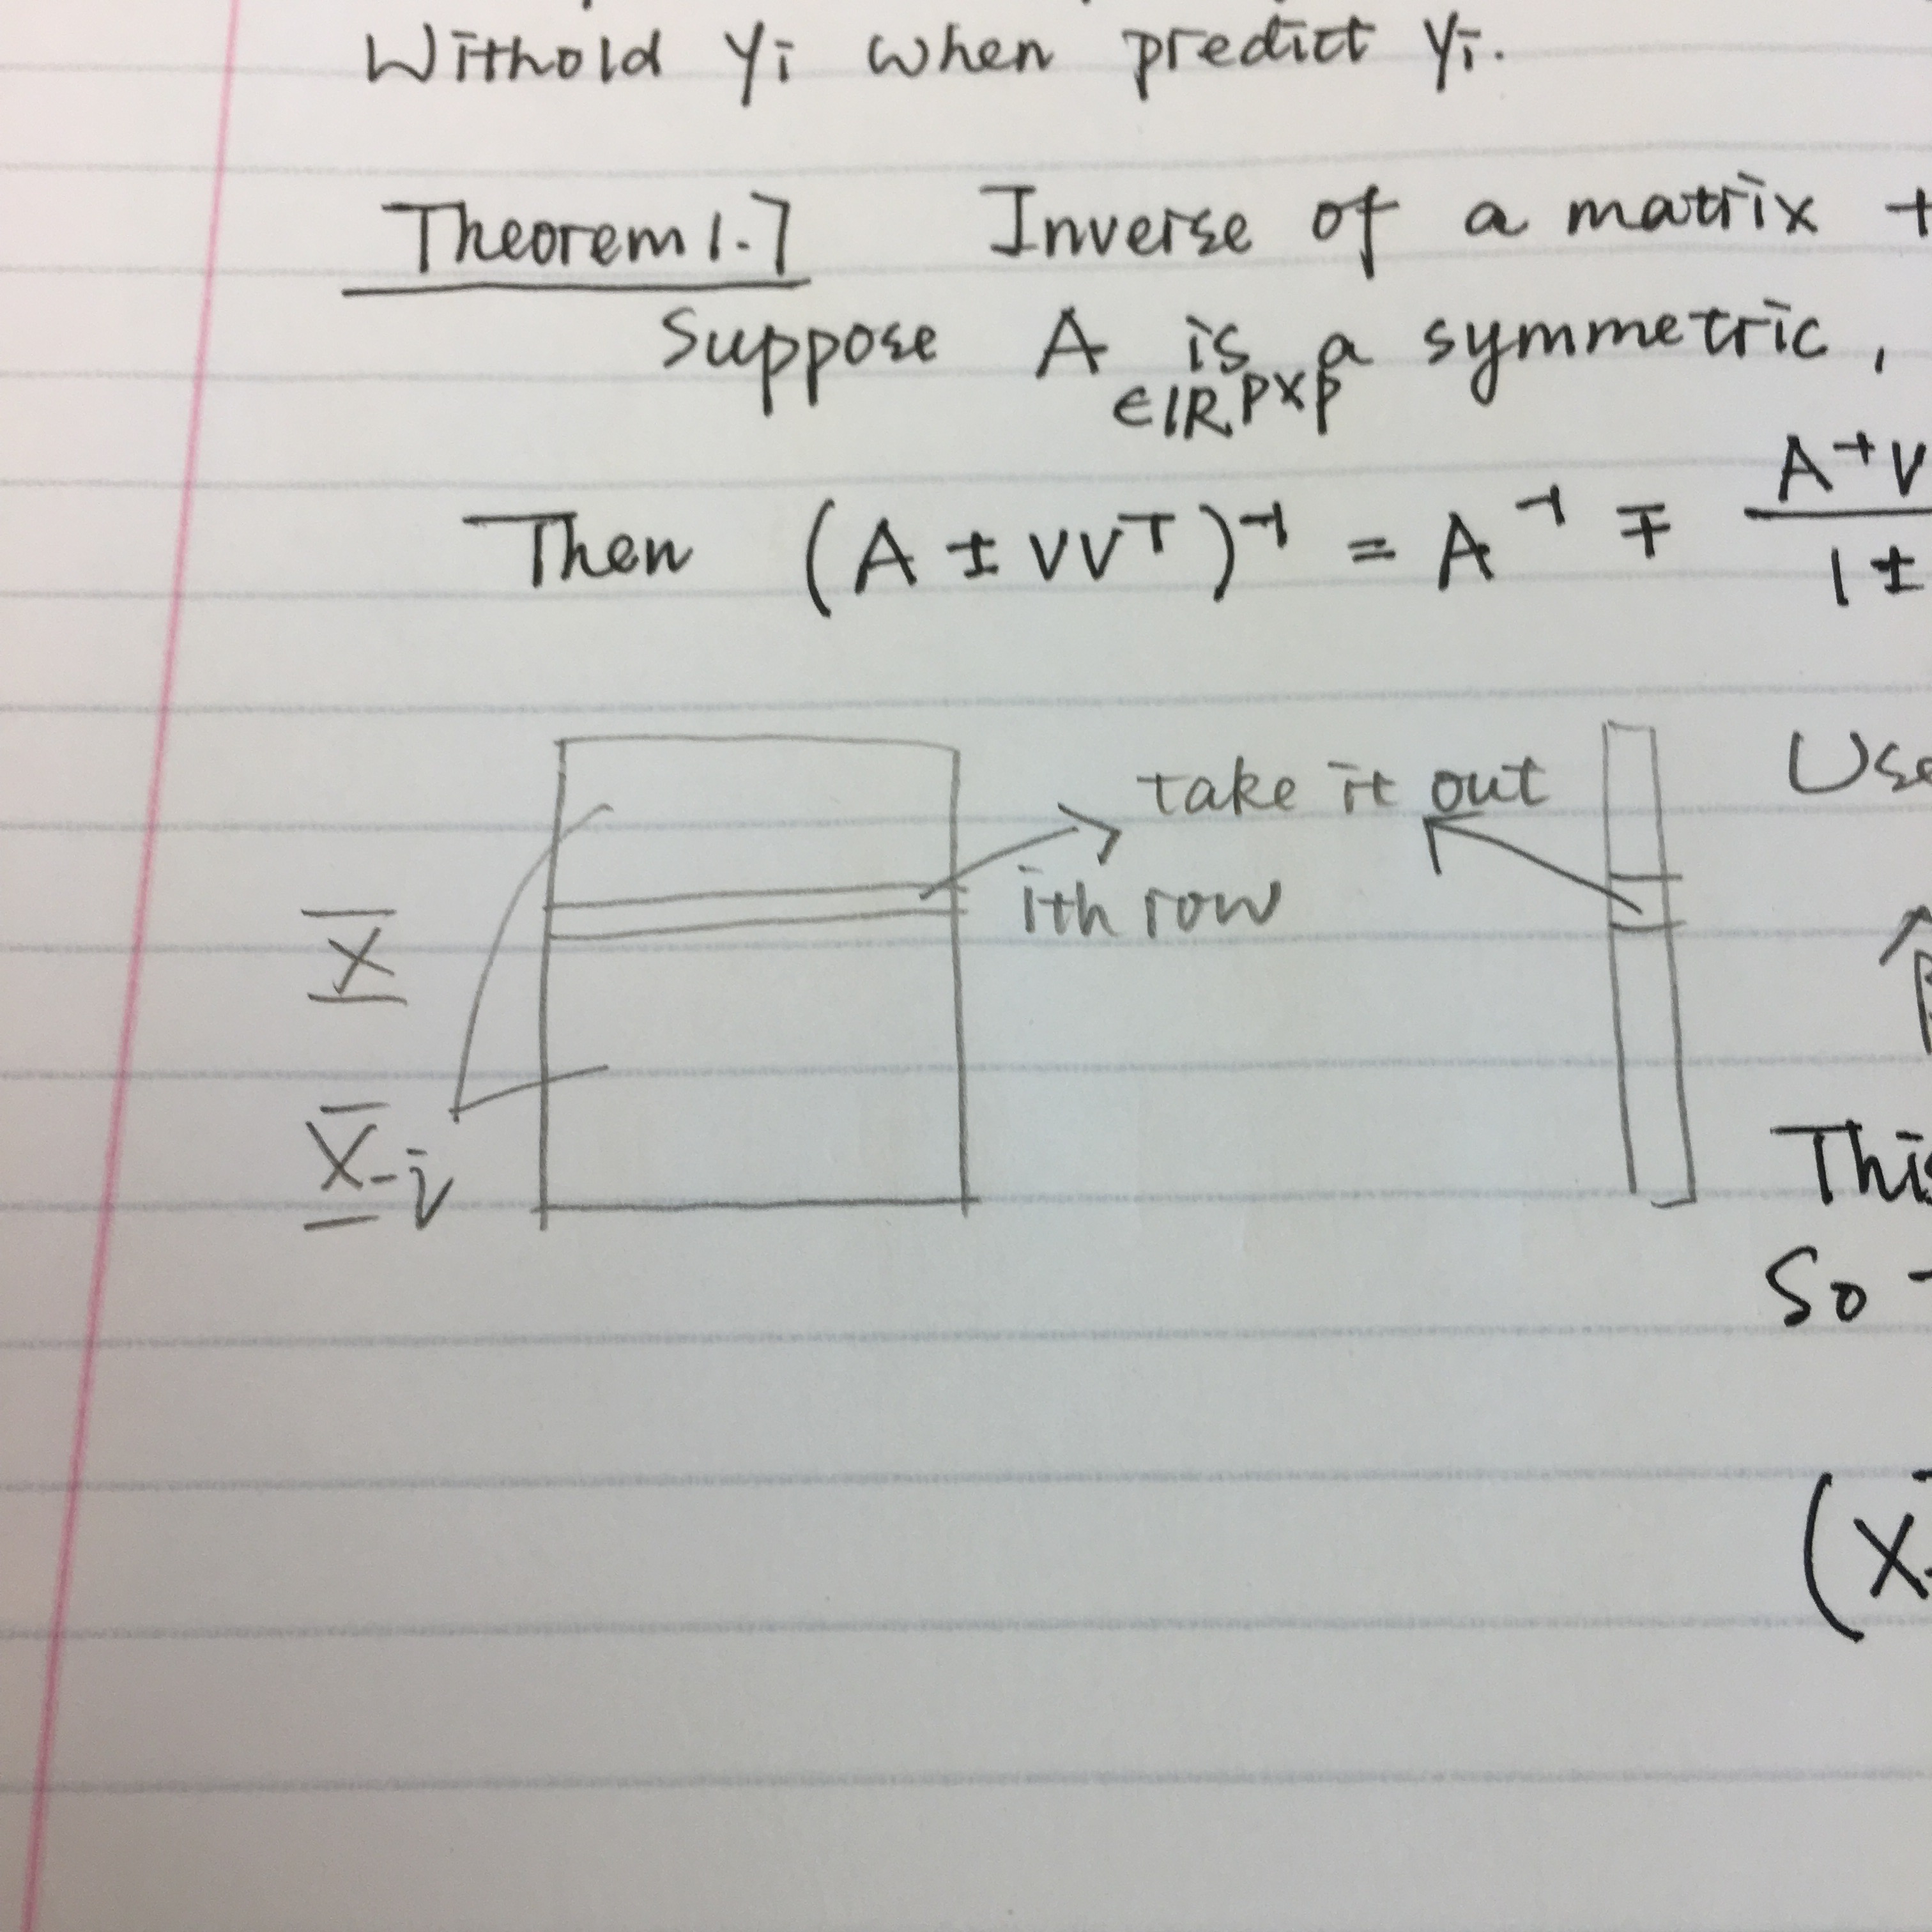
\includegraphics[scale=0.05]{wedAug31-1.jpg}
	\caption{Theorem 1.7 Visualization}
	\end{figure}

Use what is left to compute $\hat{\beta_{-i}}$.

$$\hat{\beta_{-i}} = (X^T_{-1}X_{-i})^{-1}X^T_{-i} y_{-i}$$

This can be expanded in simple sum, so that you don't have to do n regressions.

\begin{align*}
	(X^T_{-i} X_{-i})^{-1} &= (X^TX-X_iX_i^T)^{-1}\\
	&=A^{-1} + \frac{A^{-1}v v^T A^{-1}}{1 - v^t A^{-1} v}\\
	&=(X^T X)^{-1} + \frac{(X^TX)^{-1}X_i X_i^T (X^TX)^{-1}}{1 - X^T_i M X_i}\\
	X_i^T M X_i &= X_i^T (X^T X)^{-1}  \\
	&= (P_x)_{ii}\\
	&= P_i\\
	\\
	\hat{\beta}_i &= (X^TX - X_iX_i^T)^{-1} (X^T y - X_i y_i)\\
	&= [M + \frac{M X_i X_i^T M}{1 - P_i}] (X^T y - X_i y_i)\\
	&= M X^T y + \frac{M X_i X_i^T M X^T y}{1 - P_i} - M X_iy_i - \frac{M X_i X_i^T M X_i y_i}{1 - P_i}\\
	&= \dots\\
	&= \hat{\beta} - \frac{M X_i}{1 - P_i}(y_i - X_i^T \hat{\beta})
\end{align*}

Delete-one regression. 

$X_i\hat{\beta_{-i}} = \hat{y}_i - \frac{P_i}{1 - P_i} (y_i - \hat{y_i})$

\textbf{Friday September 2}\\
\\

Delete- one error

$$y_i - \hat{y}_i^{(-i)}$$

\begin{remark}
	Recall, you want to leave out $y^{i}$ so you don't overfit. 
\end{remark}


The above is equivalent to 

\begin{align*}
	y_i - X_i^T \hat{\beta}_{-i}\\
	y_i - \hat{y}_i - \frac{P_i}{1 - P_i} (y_i - \hat{y_i})\\
	(y_i - \hat{y}_i) (1 - \frac{P_i}{1 - P_i}))\\
	\frac{1}{1 - P_i} (y_i - \hat{y}_i)
\end{align*}

% GET INUITION ABOUT ABOVE

Delete-one cross validation 

$\displaystyle \sum^n_{i=1} (y_i - \hat{y}_i^{(-i)})^2$

This method is not affected by over fitting. 

The following is often used for "tuning" or variable selection (i.e. penalty, bandwidth, regularization, etc).
$ \displaystyle \sum^n_{i=1} \frac{1}{(1 - P_i)^2}(y_i - \hat{y}_i)^2$

Note: we will come back to variable selection later. 

$\beta = \begin{pmatrix} \beta_1  \\  
\vdots \\
\beta_n
 \end{pmatrix}$

$ A \subseteq \{1, \dots, P \}$

Cross validation of $A$ minimizes over $A \in 2^{\{1, \dots, P \}}$. Best cross validation set. 




\section{Residuals}\index{Residuals}

\begin{itemize}
	\item Residual
		$$\hat{e}_i = y_i - \hat{y}_i $$
	\item Standardized Residual
		$$\text{Var}(\hat{e}_i) = \text{Var}(y_i - \hat{y}_i) = \text{Var}((Q_X)_{ii}y_i)$$
		$$= ((Q_X)_{ii}y_i) \sigma^2 $$
		$$= (1 - P_i)\sigma^2 $$
		$$ sd(\hat{e}_i) = \sqrt{1-P_i} \sigma $$
		$$\hat{sd}(\hat{e}_i) = \sqrt{1-P_i} \tilde{\sigma} $$
		$$ \tilde{\sigma} = \frac{\displaystyle \sum^n_{i=1} (y_i - \hat{y}_i^{(-i)})^2}{n-p}$$
	\item Standardized residual
		$$E^*_i = \frac{\hat{e}_i}{\tilde{\sigma} \sqrt{1 - P_i}} $$
	\item Prediction Error Sum of Squares (PRESS) Residual
		$$y_i - \tilde{y}_i^{(-i)} = \frac{1}{1-P_i} \hat{e}_i = \hat{e}_{iP} $$

		$$ \hat{e}_{iP} \sim N(0, \frac{\sigma^2}{1 - P_i})$$
	\item Standardized PRESS Error
		$$\frac{\hat{e}_{iP}}{\tilde{\sigma}/ \sqrt{1-{_i}}} = \frac{\frac{1}{1-P_i}\hat{e}_i}{\tilde{\sigma}\\(\sqrt{1 - P_i})} = \frac{\hat{e}_i}{\tilde{\sigma}\\(\sqrt{1 - P_i})} = e^*_i$$
\end{itemize}

\section{Influence and Cook's Distance}\index{Influence, Cook's Distance}
% PHOTO
\begin{definition}[Influence] The difference between predictions with and without a data point.
	$$\hat{y}_i - \hat{y}_i^{(-i)} $$

\end{definition}

$$\hat{y}_i - \hat{y}_i^{(-i)} $$

$$X_i\hat{\beta} - X_i\hat{\beta}_{-i} $$

	$$\propto || X_i\hat{\beta} - X_i\hat{\beta}_{-i} ||^2	$$
	$$= (X(\hat{\beta} - \hat{\beta}_{-i}))^T (X(\hat{\beta} - \hat{\beta}_{-i})) $$
	$$(\hat{\beta} \hat{\beta}_{-i})^T X^TX (\hat{\beta} \hat{\beta}_{-i}) $$


Recall, 

$\hat{\beta}_{-i} - \hat{\beta} = -\frac{MX_i (y_i - \hat{y}_i)}{1 - P_i} = - \frac{MX_i \hat{e}_i}{1 - P_i}$

$|| X_i\hat{\beta} - X_i\hat{\beta}_{-i} ||^2 = \frac{}{} $

$= $


Cook's Distance (Technometrics, 1976?)

$$||\frac {\hat{y} - \hat{y}^{(-i)} ||^2}{\mathscr{p} \tilde{\sigma}^2} = \frac{|i \hat{e}_i^2}{(1 - P_i)^2 \mathscr{p} \tilde{\sigma}^2} $$

\begin{definition}[Cook's Distance] Cook's distance measures the influence of the $i^{th}$ deservation.
\end{definition}

\section{Orthogonal Decomposition}\index{Orthogonal Decomposition}

Recall,
$\mathbb{R}^n$ is Euclidean Space.\\

$\mathscr{S}$ is a subspace ($\mathscr{S} \leq \mathbb{R}^n$)

\begin{remark}
	$\leq$ is subspace\\
	$\subseteq$ is a subset
\end{remark}

For 

$\mathscr{S}_1 \leq \mathscr{S}_1 \mathscr{S}_2 \leq \mathscr{S}$

$$\mathscr{S}_1 + \mathscr{S}_2 = \{x + y: x \in \mathscr{S}_1, y \in \mathscr{S}_2 \} $$

% PHOTO

Suppose $\mathscr{S}_1, \mathscr{S}_2 \leq \mathscr{S}$, 

$\mathscr{S}_1 + \mathscr{S}_2 = \mathscr{S}$, $\mathscr{S}_1 \perp \mathscr{S}_2$

then, 

	$$\{\mathscr{S}_1, \mathscr{S}_2 \} $$ is called an orthogonal decomposition of $\mathscr{S}$

% PHOTO

In this case, 

	$$\mathscr{S}_1 \oplus \mathscr{S}_2 = \mathscr{S} $$

More generally, 

\begin{definition}[Orthogonal Decompositon (O.D.)]
	Let $\mathscr{S}_1, \dots, \mathscr{S}_k$ be subspaces of $\mathscr{S}$ such that

	\begin{enumerate}
		\item $\mathscr{S}_1, \dots, \mathscr{S}_k = \{v_1 + \dots + v_k : v_1 \in \mathscr{S}_1, \dots, v_k \in \mathscr{S}_k\}$
		\item $\mathscr{S}_i \perp \mathscr{S}_j \quad \forall i\neq j$
	\end{enumerate}
	
	Then, $\{\mathscr{S}_1, \mathscr{S}_2, \dots, \mathscr{S}_k\}$ is an \textbf{orthogonal decomposition} of $\mathscr{S}$. We may write $\mathscr{S} = \mathscr{S}_1 \oplus \mathscr{S}_2 \oplus \dots \oplus \mathscr{S}_k$.
\end{definition}

\textbf{Proposition 1.5} If $\mathscr{S}_1, \dots, \mathscr{S}_k$ is an O.D. of $\mathscr{S}$, then any $v \in \mathscr{S}$ can be uniquely written as

$$v_1 + \dots + v_k$$, where $v_1 \in \mathscr{S}_1, \dots v_k \in \mathscr{S}_k$. \\

\textbf{Wednesday September 7}

\begin{definition}[Direct Difference]
	Let $\mathscr{S}_1 \leq \mathscr{S}_2 \leq \mathbb{R}^n$. Then, \\

	$$\mathscr{S}_2 \cap \mathscr{S}_1^\perp \equiv \mathscr{S}_2 \ominus \mathscr{S}_1 $$ 

	is called \textbf{direct difference}. This is almost the same as orthogonal complement, except it is within $\mathscr{S}_2$. 

\end{definition}

\textbf{Proposition 1.6} If $\mathscr{S}_1 \leq \mathscr{S}_2$, then 

$$\mathscr{S}_2 = \mathscr{S}_1 \oplus (\mathscr{S}_2 \ominus \mathscr{S}_1) $$

\textbf{Proposition 1.7 - Orthogonal Decomposition and Projection} Consider a Hilbert Space, $\mathscr{H} = \{\mathbb{R}^n, <,>_A \}$, 

\begin{enumerate}
	\item If $\mathscr{S} \leq \mathscr{S}_1 \perp \mathscr{S}_2$ in $\mathscr{H}$, then 

	$$P_{\mathscr{S}_1} (A) P_{\mathscr{S}_2} (A) = 0  $$

	\item If $\mathscr{S} \leq \mathscr{H}, \dots, \mathscr{S}_k \leq \mathscr{H}$, and $\mathscr{S}_1 \perp \dots \perp \mathscr{S}_k$, then

	$$P_{\mathscr{S}_1, \oplus \dots \oplus \mathscr{S}_k} (A) = P_{\mathscr{S}_1} (A) + \dots + P_{\mathscr{S}_k} (A) $$

	\item If $\mathscr{S}_1 \leq \mathscr{S}_2 \leq \mathbb{R}^n$, then

	$$P_{\mathscr{S}_2 \ominus \mathscr{S}_1} (A) = P_{\mathscr{S}_2} (A) - P_{\mathscr{S}_1} (A)$$
\end{enumerate}


\begin{theorem}[Generalization of the earlier Cochran's Theorem]

Suppose $X \sim N(0, \Sigma)$ where $\Sigma \in \mathbb{R}^{nxn}$ is positive definite. 

Let $\mathscr{H} = \{ <,>_{\Sigma^{-1}}\}$. Suppose $\mathscr{S}_1, \dots \mathscr{S}_k, \mathscr{S} \leq \mathscr{H}$ such that $\mathscr{S} = \mathscr{S}_1 \oplus \dots \oplus \mathscr{S}_k$.\\

Let 

	$$w_i = ||P_{\mathscr{S}_i} (\Sigma^{-1}) X ||^2_{\Sigma^{-1}} $$
	$$w = ||P_{\mathscr{S}} (\Sigma^{-1}) X ||^2_{\Sigma^{-1}} $$

Then, 

\begin{enumerate}
	\item $ w = w_1 + \dots + w_k$
	\item $ w_1 \indep \dots \indep w_k$
	\item $w_i \sim \chi^2_{r_i}$\\
		$w \sim \chi^2_{r}$\\
		where $r_i$ is the $dim(\mathscr{S}_i)$, $r$ is the $dim(\mathscr{S})$, and $r = r_1 + \dots + r_k$.
\end{enumerate}
	
\end{theorem}

\begin{notation}
	We use $\oplus$ for spaces. We can also use $\oplus$ function to stack up matrices. Let $A_1, \dots, A_k$ be matrices with arbitrary dimensions. 

	$$A_1 \oplus \dots \oplus A_k = \begin{pmatrix}
		A_1 & \dots & 0\\
		    & \ddots & \\
		0 & \dots & A_k
	\end{pmatrix} $$
\end{notation}

\section{Lack of Fit Test}\index{Lack of Fit Test}

Goodness of Fit

% GET PHOTO

At each $x_i$ you have multiple observations, say $y_{i1}, \dots, y_{im_i}$. In this case, you may test to see if a linear model,$y_i = x_i^T \beta + \epsilon_i$ , is the correct choice for fitting the data. In general, lack of fit refers to testing whether any (linear, generalized, etc) model is adequately describing the data. 

Denote 

$y_i = \begin{pmatrix}
	y_{i1}\\
	\vdots\\
	y_{im_i}
\end{pmatrix}$

$1_{m_i} = \begin{pmatrix}
	1 \\
	\vdots\\
	1
\end{pmatrix}$

$X = \begin{pmatrix}
	X_{1}^T\\
	\vdots\\
	X_{m}^T
\end{pmatrix}$

Assume

$$y_{ij} = X_i^T \beta + \epsilon_{ij} $$

where $\epsilon \sim^{iid} N(0, \sigma^2)$. 

The point is that you have $y_{i1} \dots y_{jm}$ for each $X_i$.\\

In matrix form, 

% GET PHOTO

$$(1_{m_1} \oplus \dots \oplus 1_{m_n}) X\beta + \epsilon $$

So, let $N$ denote a full sample size. 

$$N = m_1 + \dots + m_n$$

this is a special case of linear model, except the design matrix is structured $(1_{m_1} \oplus \dots \oplus 1_{m_n})X $ instead of X. So the formula for MLE (and so on) is the same. \\

$$X \leftrightarrow (1_{m_1} \oplus \dots \oplus 1_{m_n})X$$

So, 

$$\hat{\beta} = ([(1_{m_1} \oplus \dots \oplus 1_{m_n})X])^T ([(1_{m_1} \oplus \dots \oplus 1_{m_n})X])^{-1} [(1_{m_1} \oplus \dots \oplus 1_{m_n})X]^T y$$

\begin{align*}
\hat{y} &= (1_{m_1} \oplus \dots \oplus 1_{m_n})X \hat{\beta} \\
	&= (1_{m_1} \oplus \dots \oplus 1_{m_n})X ([(1_{m_1} \oplus \dots \oplus 1_{m_n})X])^T ([(1_{m_1} \oplus \dots \oplus 1_{m_n})X])^{-1} [(1_{m_1} \oplus \dots \oplus 1_{m_n})X]^T y\\
	&=  (1_{m_1} \oplus \dots \oplus 1_{m_n})X [X^T \begin{pmatrix}
		m_1 & \dots & 0\\
		  & \ddots  & \\
		  0 & \dots & m_n
	\end{pmatrix} 	X]^{-1} X^T (1_{m_1} \oplus \dots \oplus 1_{m_n})	
\end{align*}

So, in linear model with replication we have our hypotheses for lack of fit test, 

$$H_O: E(y_i) = 1_{m_i} X_i^T \beta$$
$$H_1: E(y_i) = 1_{m_i} \mu_i $$

% GET PHOTO 

We are testing whether the arbitrary means, $\mu_1, \dots \mu_n$ sit on the same line. \\


\textbf{Friday September 9}

Under $H_1$, 

$$ y = (1_{m_1} \oplus \dots \oplus 1_{m_n}) \begin{pmatrix}
	\mu_1\\
	\vdots\\
	\mu_n
\end{pmatrix}
+ \epsilon$$

So the $\hat{y}$ under this model, 

$$\hat{y}_{H_1} = P_{1_{m_1} \oplus \dots \oplus 1_{m_n}} y = (1_{m_1} \oplus \dots \oplus 1_{m_n}) \begin{pmatrix}
	m_1 & & \\
	 & \ddots & \\
	  &  & m_n
\end{pmatrix} (1_{m_1} \oplus \dots \oplus 1_{m_n})^T y$$

but under $H_0$, 

$$ \hat{y}_{H_0} = P_{(1_{m_1} \oplus \dots \oplus 1_{m_n})X} y$$

$$\mathscr{S}_1 = \text{span}\{(1_{m_1} \oplus \dots \oplus 1_{m_n})X \} \quad \text{(p-dim)}$$

$$\mathscr{S}_2 = \text{span}\{(1_{m_1} \oplus \dots \oplus 1_{m_n}) \} \quad \text{(n-dim)}$$

$$\mathscr{S}_3 = \mathbb{R}^N \quad (N = m_1 + \dots + m_n)$$

$$ \mathscr{S}_1 \leq \mathscr{S}_2 \leq \mathscr{S}_3 $$

\begin{remark}
	Above used the fact that span(AB) $\subseteq$ span(A)
\end{remark}

\textbf{Lemma 1.1} If $ \mathscr{S}_1 \leq \mathscr{S}_2 \leq \mathscr{S}_3$ then

\begin{enumerate}
	\item $\mathscr{S}_3 \ominus \mathscr{S}_2 \leq \mathscr{S}_3 \ominus \mathscr{S}_1$		  \item $(\mathscr{S}_3 \ominus \mathscr{S}_1) \ominus \mathscr{S}_2 =  \mathscr{S}_3 \ominus \mathscr{S}_2$
	\item $(\mathscr{S}_3 \ominus \mathscr{S}_1) = (\mathscr{S}_3 \ominus \mathscr{S}_2) \oplus (\mathscr{S}_2 \ominus \mathscr{S}_1)$
 
\end{enumerate}

Go back to lack of fit, 

$$(\mathscr{S}_3 \ominus \mathscr{S}_1) = (\mathscr{S}_3 \ominus \mathscr{S}_2) \oplus (\mathscr{S}_2 \ominus \mathscr{S}_1)$$

$$P_{\mathscr{S}_3 \ominus \mathscr{S}_1}y = P_{\mathscr{S}_3 \ominus \mathscr{S}_3}y + P_{\mathscr{S}_2 \ominus \mathscr{S}_1}y \quad \text{(Orthogonal Decomposition)} $$

$$||P_{\mathscr{S}_3 \ominus \mathscr{S}_1}y||^2 = ||P_{\mathscr{S}_3 \ominus \mathscr{S}_3}y||^2 + ||P_{\mathscr{S}_2 \ominus \mathscr{S}_1}y||^2 $$

$$dim(\mathscr{S}_2 \ominus \mathscr{S}_1) = n-p$$

$$dim(\mathscr{S}_3 \ominus \mathscr{S}_2) = N-n$$

Now, 

$$E(P_{\mathscr{S}_3 \ominus \mathscr{S}_2}y) = P_{\mathscr{S}_3 \ominus \mathscr{S}_2}E(y) =P_{\mathscr{S}_3 \ominus \mathscr{S}_2} \mu  = 0 $$

But, 

$\mu = \begin{pmatrix}
	\mu_1\\
	\vdots\\
	\mu_n
\end{pmatrix} \in \mathscr{S}_2$

and, 

$(1_{m_1} \oplus \dots \oplus 1_{m_n})\underline{\mu}$

$$Var(P_{\mathscr{S}_3 \ominus \mathscr{S}_2}y) = P_{\mathscr{S}_3 \ominus \mathscr{S}_2}Var(y)P_{\mathscr{S}_3 \ominus \mathscr{S}_2} = \sigma^2 P^2_{\mathscr{S}_3 \ominus \mathscr{S}_2} = \sigma^2 P_{\mathscr{S}_3 \ominus \mathscr{S}_2} $$

We know that $y \sim N(\mu, \sigma^2 I_n)$. So, 

$$P_{\mathscr{S}_3 \ominus \mathscr{S}_2}y \sim N(0, \sigma^2 P_{\mathscr{S}_3 \ominus \mathscr{S}_2} $$

Similarly, 

$$ E(P_{\mathscr{S}_2 \ominus \mathscr{S}_1}y) = P_{\mathscr{S}_2 \ominus \mathscr{S}_1}E(y)$$

which under $H_0$ is, 

$$P_{\mathscr{S}_2 \ominus \mathscr{S}_1} (1_{m_1} \oplus \dots \oplus 1_{m_n})X\beta = 0 $$

$$Var(P_{\mathscr{S}_2 \ominus \mathscr{S}_1}y) = \sigma^2 P_{\mathscr{S}_2 \ominus \mathscr{S}_1} $$

$$P_{\mathscr{S}_2 \ominus \mathscr{S}_1} y \sim N(0, \sigma^2 P_{\mathscr{S}_2 \ominus \mathscr{S}_1})$$

By Chochran's Theorem: 

	Under $H_O$, 

	$$||P_{\mathscr{S}_3 \ominus \mathscr{S}_2} y||^2 \sim \chi^2_{(N-n)} $$
	$$||P_{\mathscr{S}_2 \ominus \mathscr{S}_1} y||^2 \sim \chi^2_{(n-p)} $$

	$$||P_{\mathscr{S}_3 \ominus \mathscr{S}_2} y||^2 \indep  ||P_{\mathscr{S}_2 \ominus \mathscr{S}_1} y||^2$$

So our lack of fit test is: 

	$$\frac{||P_{\mathscr{S}_2 \ominus \mathscr{S}_1} y||^2 / (n-p)}{||P_{\mathscr{S}_3 \ominus \mathscr{S}_2} y||^2 / (N - n)} \sim F _{n-p, N-n} $$



 \section{Explicit Intercept}\index{Explicit Intercept}


We now apply this $\mathscr{S}_1, dots $ argument to another problem: special linear model. 

$$y_i = \alpha + \beta^TX_i + \epsilon_i 	\quad i = 1, \dots, n $$

$y = \begin{pmatrix}
	y_1\\
	\vdots\\
	y_n
\end{pmatrix}$

$X = \begin{pmatrix}
	X_1\\
	\vdots\\
	X_n
\end{pmatrix}$

$\epsilon = \begin{pmatrix}
	\epsilon_1\\
	\vdots\\
	\epsilon_n
\end{pmatrix}$

$$Y = 1_n \alpha + X\beta + \epsilon = (1_n X)\begin{pmatrix}
	\alpha\\
	\beta
\end{pmatrix} + \epsilon = U\eta + \epsilon$$

Let $P_{1_n} = 1_n(1_n^T 1_n)^{-1} 1_n^T = \frac{1_n1_n^T}{n}$.\\

Note that for all $a = \begin{pmatrix}
	a_1\\
	\vdots\\
	a_n
\end{pmatrix} \in \mathbb{R}^n$, 

	$$P_{1_n}a = \frac{1_n 1_n^T a}{n} = 1_n \bar{a}, \quad \bar{a}= \frac{1}{n}\displaystyle\sum^n_{i=1}a_i $$

	which is a mean projection. (?)

	$Q_{1_n} = I_n - P_{1_n} \quad \text{(projection on}1_n^\perp\text{)}$\\

	$$ Q_{1_n} a = \begin{pmatrix}
		a_1 - \bar{a}\\
		\vdots \\
		a_n - \bar{a}

	\end{pmatrix}$$

	Decompose X:

	$$X = P_{1_n}X + Q_{1_n}X $$

	$$U \eta = 1_n \alpha + X\beta = 1_n \alpha + P_{1_n}X\beta + Q_{1_n}X\beta = 1_n (\alpha + \frac{1_n^T X\beta}{n}) + Q_{1_n}X\beta = (1_n Q_{1_n}X)\begin{pmatrix}
		\alpha^\star\\
		\beta
	\end{pmatrix} = (1_n Q_{1_n}X)\eta^\star = U^\star\eta^\star $$

	So we do least squres of

	$$(y - U^\star\eta^\star)^T(y - U^\star\eta^\star)$$

	and minimize this over all $\eta^\star \in \mathbb{R}^{Px1}$


	$$\hat{\eta}^\star = (U^{\star T} U^\star)U^{\star T} y $$

	$$U^{\star T} U^\star = \begin{pmatrix}
		1_n^T\\
		(Q_{1_n}X)^T
	\end{pmatrix} (1_n Q_{1_n}X) = \begin{pmatrix}
		1_n^t1_n & Q_{1_n}X1_n\\
		1_n^TQ_{1_n}X & Q_{1_n}X Q_{1_n}X\\
	\end{pmatrix}  = \begin{pmatrix}
		n & 0 \\
		0 & X^TQ_{1_n}X
	\end{pmatrix}$$

	$$\hat{\eta}^\star = \begin{pmatrix}
		n^{-1} & 0 \\
		0 & (X^T Q_{1_n}X)^{-1}
	\end{pmatrix} \begin{pmatrix}
		1_n \\
		(Q_{1_n}X)^T
	\end{pmatrix} y$$

	\textbf{Monday September 12}

	So 

	$$\hat{\alpha}^\star = n^{-1}1_n^T y $$

	$$\hat{\beta} = (X^TQX)^{-1} X^TQ y $$

	$$\hat{\alpha} = n^{-1} 1^T_n y - n^{-1}X \hat{\beta}^\star $$

	For statistical inference, we want to make a decomposition of $\mathbb{R}^n$.

	Let, $\mathscr{S}_1 = \text{span}(1_n), \mathscr{S}_2 = \text{span}(1_n, X), \mathscr{S}_3 = \mathbb{R}^n$. \\

	Then,

	$$(\mathscr{S}_3 \ominus \mathscr{S}_1) = (\mathscr{S}_3 \ominus \mathscr{S}_2) \oplus (\mathscr{S}_2 \ominus \mathscr{S}_1) $$

	Then, 

	$$||P_{\mathscr{S}_3 \ominus \mathscr{S}_1}y||^2 = ||P_{\mathscr{S}_3 \ominus \mathscr{S}_2}y||^2 + ||P_{\mathscr{S}_2 \ominus \mathscr{S}_1}y||^2 $$

	Or, 

	$$SSTotal = SSError + SSRegression $$ 

	We may compute these terms, 

	\begin{align*}
		P_{\mathscr{S}_3 \ominus \mathscr{S}_1} =  P_{\mathscr{S}_3} - P_{\mathscr{S}_1}\\
			&= I_n - \frac{1_n1_n}{1_n^T1_n}\\
			&= Q_1n\\
		\mathscr{S}_2 \ominus \mathscr{S}_1	&= \text{span}(Q_{1_n}X)\\
		P_{\mathscr{S}_2 \ominus \mathscr{S}_1} &= QX(X^TQX)^{-1}QX^T\\
		P_{\mathscr{S}_3 \ominus \mathscr{S}_2}&= Q - QX(X^TQX)^{-1}X^TQ
	\end{align*}

By Cochran's Theorem, (these are orthogonalized projections, etc), 

$$ ||P_{\mathscr{S}_3 \ominus \mathscr{S}_1}y||^2 \sim \chi^2{(n-1)} $$
$$ ||P_{\mathscr{S}_2 \ominus \mathscr{S}_1}y||^2 \sim \chi^2_{(p-1)} $$
$$ ||P_{\mathscr{S}_3 \ominus \mathscr{S}_2}y||^2 \sim \chi^2_{(n - p - 1)} $$

\begin{remark}
	$$dim(\mathscr{S}_3) = n$$
	$dim(\mathscr{S}_2) = p+1$
	$dim(\mathscr{S}_3) = 1$
\end{remark}

We also know that these are all independent of each other. So we can test regression effect with the following hypothesis:

$$H_0: \beta - 0 $$


$$\frac{||P_{\mathscr{S}_2 \ominus \mathscr{S}_1}y||^2 / (p-1)}{||P_{\mathscr{S}_3 \ominus \mathscr{S}_2}y||^2 / (n-p - 1)} = \frac{y^T QX(X^TQX)^{-1}QX^T y /(p-1)}{y^T (Q - QX(X^TQX)^{-1}X^TQ) y / (n-p - 1)} \sim F_{p-1, n - p - 1} $$

Distributions\\

$$\hat{\beta} (X^TQX)^{-1}X^TQy$$

$E(\hat{\beta}) = (X^TQX)^{-1}X^TQ(1_{n\alpha} + X\beta = (X^TQX)^{-1}X^TQX \beta = \beta$

$\text{Var}(\hat{\beta}) =  (X^TQX)^{-1}X^TQ (\sigma^2 I_n) QX (X^TQX)^{-1} = \sigma^s(X^TQX)^{-1} $

$\hat{\alpha} = \hat{\alpha}^\star - X^T \hat{\beta}$

Because $\hat{\beta}$ is a function of $Qy$ and $\hat{\alpha}^\star$ is a function of $P_{1_n}y$ (and these are orthogonal to each other and thus by normality also independent). \\

$\text{Var}(\hat{\alpha} = \text{Var}(\hat{\alpha}^\star) + \text{Var}( \bar{X}^T \hat{\beta}) = \text{Var}(\bar{y}) + \text{Var}( \bar{X}^T \hat{\beta}) = \frac{\sigma^2}{n} + \sigma^2 \bar{X}^T(X^TQX)^{-1} \bar{X} $

$$\hat{\alpha} ~ N( \alpha, \frac{\sigma^2}{n} + \sigma^2 \bar{X}^T(X^TQX)^{-1} \bar{X}) $$

\begin{align*}
	Cov(\hat{\alpha}, \hat{\beta}) &= Cov(\hat{\alpha}^\star - \bar{X}^T\hat{\beta}, \hat{\beta})\\
		&=-\bar{X}^T Var(\hat{\beta})\\
		&= =\bar{X}^T \sigma^2 (X^TQX)^{-1}
\end{align*}

$$ \begin{pmatrix}
	\hat{alpha}\\
	\hat{\beta}
\end{pmatrix} \sim N[\begin{pmatrix}
	\alpha\\
	\beta
\end{pmatrix}, \begin{pmatrix}
	\frac{\sigma^2}{n} + \sigma^2 \bar{X}^T(X^TQX)^{-1} \bar{X} & - \sigma^2 \bar{X}^T(X^TQX)^{-1} \bar{X}\\
	- \sigma^2 \bar{X}^T(X^TQX)^{-1} \bar{X} & \frac{\sigma^2}{n} + \sigma^2 \bar{X}^T(X^TQX)^{-1} \bar{X}
\end{pmatrix}]$$

Estimate $\sigma^2$\\


$$ ||P_{\mathscr{S}_3 \ominus \mathscr{S}_2}y||^2 = \displaystyle \sum^n_{i=1} (y_i - \hat{\alpha} - \hat{\beta}^TX_i)^2 \sim \sigma^2 \chi^1_{n-p-1}$$

So, 

$$E(||P_{\mathscr{S}_3 \ominus \mathscr{S}_2}y||^2 ) = \sigma^2 (n-p-1)$$

Thus, 

$$\hat{\sigma}^2 = \frac{||P_{\mathscr{S}_3 \ominus \mathscr{S}_2}y||^2 }{n-p-1}$$

\begin{theorem}
	Under the explicit intercept model, 

	\begin{enumerate}
		\item $(\hat{\alpha}, \hat{\beta}, \hat{\sigma}^1)$ is UMVUE of $(\alpha, \beta, \sigma^2)$ by Lehmann-Sheffe.
		\item $$ \begin{pmatrix}
	\hat{\alpha}\\
	\hat{\beta}
\end{pmatrix} \sim N[\begin{pmatrix}
	\alpha\\
	\beta
\end{pmatrix}, \begin{pmatrix}
	\frac{\sigma^2}{n} + \sigma^2 \bar{X}^T(X^TQX)^{-1} \bar{X} & - \sigma^2 \bar{X}^T(X^TQX)^{-1} \bar{X}\\
	- \sigma^2 \bar{X}^T(X^TQX)^{-1} \bar{X} & \frac{\sigma^2}{n} + \sigma^2 \bar{X}^T(X^TQX)^{-1} \bar{X}
\end{pmatrix}]$$
	\item $(n-p-1) \hat{\sigma}^2 \sim \sigma^2 \chi^2_{(n-p-1)}$
	\item $\begin{pmatrix}
			\hat{\alpha}\\
			\hat{\beta}
		\end{pmatrix} \indep \hat{\sigma}^2$
	\end{enumerate}
\end{theorem}



% %------------------------------------------------




\section{$R^2$}\index{$R^2$}

Proportion of Sum of Squares (SS) explained by regression (i.e. by $\beta$). 

$$R^2 = \frac{SSR}{SST} = \frac{||P_{\mathscr{S}_2 \ominus \mathscr{S}_1}y||^2}{||P_{\mathscr{S}_3 \ominus \mathscr{S}_1}y||^2}$$

But we know that, 

$$R^2 = \frac{||P_{\mathscr{S}_2 \ominus \mathscr{S}_1}y||^2}{||P_{\mathscr{S}_2 \ominus \mathscr{S}_1}y||^2 + ||P_{\mathscr{S}_3 \ominus \mathscr{S}_2}y||^2} = \frac{SSR}{SSR + SSE} = \frac{SSR/SSE}{SSR/SSE + 1} $$

$$ F = \frac{SSR/p}{SSE/(n-p-1)} = \frac{(n-p-1)}{p} \frac{SSR}{SSE} $$

$$ \frac{SSR}{SSE} = \frac{p}{(n-p-1)} F$$

$$R^2 = \frac{\alpha F}{\alpha F + 1}$$
where $\alpha = \frac{p}{n-p-1}$

This is how we compute the null distribution of $R^2$. \\

\section{Multicollinearity}\index{Multicollinearity}

\textbf{Wednesday September 14}\\

$y = C_1 \beta_1 + \dots + C_p \beta_p$

$$ X = (C_1, \dots, C_P) = \begin{matrix}
	X^T_1\\
	\vdots\\
	X^T_n
\end{matrix}$$

In an extreme case, multicolinearity simply means that the $C_1, \dots, C_p$ are linearly dependent. In this case $\beta$ is not identifiable. 

	We have $C_1, C_2, C_3$.\\

	\begin{align*}
		C_1 &= a\\
		C_2 &= 2a\\
		C_3 &= b
	\end{align*}

	\begin{align*}
		y &= a\beta_1 + 2a \beta_2 + b\beta_3 + \epsilon\\
		&= a(\beta_1 + 2\beta_2) + b\beta_3 + \epsilon
	\end{align*}
	
	$\beta_1 \& \beta_2$ cannot be split. \\

	In the less extreme case, $X^TX$ is nearly singular, meaning it has small eigenvalues. In this case, although $\beta$ is identifiable, they have large variance For example, if $C_1 = a C_2 x 2a$ then $\beta_1, \beta_2$ have large variance which means your parameterization is not good. So may define new parameterization.

	$$ \gamma_1 = \beta_1 + 2\beta_2$$
	$$ \gamma_2 = \beta_3$$ 

	If you run regression against these then the variance would be 'normal'.\\

	S0, how to wee out redundant varaibles? One way Variance Inflation Factor (VIF) which for each $ i = 1, 2, \dots, p$ regresses $C_i$ on $\{C_1, \dots, C_p \setminus C_i \}$
then you get $R^2$ for this regression call it $R_i^2$.\\

If $C_i$ is redunent then $R_i^2$ would be close to 1. 

$$VIF_i = \frac{1}{1 - R_i^2} $$





% %------------------------------------------------





\section{Variable Selection}\index{Variable Selection}

$$ y = C_1\beta_1 + \dots + C_p\beta_p + \epsilon$$

Some of these $\beta$'s are zero. \\

Let us define an active set of parameters, 

$$A_0 = \{i: \beta_i \neq 0 \}$$

To estimate $A_0$ is the goal of variable selction. \\

\textbf{Mallow's $C_p$ criterion}\\

The fundamental issue is variable selction, penalty - penalizing the number of parameters, so you cannot use something like $y - \hat{y}$ as criterion. The more variables you have the smaller $||\hat{y} - y ||^2$ is. So we want to penalize the number of parameters in a reasonable way. \\

Let any subset $A \subset \{1, \dots, p\}$, 

$$X_A = \{C_i: i \in A \}$$

\begin{notation}
	While we often use X  for iid variables (a vector), but here X is a matrix and $X_i$ were referring to its columns. We've changed $X_i$ to $C_i$ to better reflect that we are dealing with columns of X. 
\end{notation}

So, $A = \{1, 3, 5\}$, 

$$X_A = \begin{pmatrix}
	C_1\\
	C_3\\
	C_5
\end{pmatrix}$$

Let $P_{X_A}, Q_{X_A}$ be the projection on to span($X_A$), span$(X_A)^\perp$. For example, 

$$P_{X_A} = X_A(X_A^T X_A)^{-1}X_A^T $$

Let $\mu = E(y) = X\beta = X_{A_0}\beta_{A_0}$.\\

\textbf{Mallow} says we minimize

$$\frac{E||P_{A}y - \mu ||^2}{\sigma^2} $$

among all $A \subset \{1, \dots, p \}$.\\

But we do not know what $\sigma^2$ or $\mu$ are. If so, we would already know $A_0$. We must estimate these.\\

$$E || P_{X_A} y - \mu ||^2 = tr(E(P_{X_A} y - \mu)(P_{X_A} y - \mu)^T) $$

\begin{align*}
	E(P_{X_A} y - \mu)(P_{X_A} y - \mu)^T &= E[(P_{X_a}y - P_{X_a}\mu) + (P_{X_a}\mu - \mu)][(P_{X_a}y - \mu)+ (P_{X_a}\mu - \mu)]^T\\
		&=  \text{expand, two terms are zero}\\
		&= E(P_{X_a}y - P_{X_a}\mu)(P_{X_a}y - P_{X_a}\mu) + (P_{X_a}\mu  - \mu)(\P_{X_a}\mu - \mu)^T\\
		&= Var(P_{X_a}y)\\
		&= P_{X_a} \sigma^2 I_n P_{X_a} = \sigma^2 P_{X_a}\\
		&= tr(\sigma^2 P_{X_a} + Q_{X_a}\mu\mu^TQ_{X_a})\\
		&= \sigma*2 tr(P_{X_a}) + tr(Q_{X_a}\mu\mu^tQ_{X_a})\\
		&= \sigma^2(\#(A)) + tr(\mu^T Q_{X_a} \mu)\\
\end{align*}

$$\Rightarrow E\frac{ || P_{X_A} y - \mu ||^2}{\sigma^2} = \#(A) + \frac{tr(\mu^T Q_{X_a} \mu)}{\sigma^2}$$

Now let's estimate $\frac{\mu^T Q_{X_a} \mu}{\sigma^2}$. \\

Recall, if $U$ is a random vector with multivariate normal distribution so

$$E(U) = e $$
$$Var(U) = Q_{X_A} $$

$$U^TU \sim \chi^2_{(rank(Q)_{X_A})} (||e||^2) $$

Also, $W \sim \chi^2_{(r)} (\delta)$ where $E(W) = r + \delta$.\\

Go back to our problem of estimating $\frac{\mu^T Q_{X_a} \mu}{\sigma^2}$. \\

What about $y^t Q_{X_A} y$? We know that

$$E (\frac{Q_{X_A}y}{\sigma}) = \frac{Q_{X_A}\mu}{\sigma}$$

and

$$Var(\frac{Q_{X_A}y}{\sigma}) = \frac{1}{\sigma^2} Q_{X_A}\sigma^2 I_n = 0$$

So, 

$$ \frac{Q_{X_A}y}{\sigma} \sim N( \frac{Q_{X_A}\mu}{\sigma}, 0)$$

So

$$(\frac{Q_{X_A}y}{\sigma})^T(\frac{Q_{X_A}y}{\sigma}) \sim \chi^2_{(n-\#(A))} ((\frac{Q_{X_A}\mu}{\sigma})^T(\frac{Q_{X_A}\mu}{\sigma})) = \chi^2_{(n-\#(A))} (\frac{\mu^T Q_{X_A} \mu}{\sigma^2}) $$

Thus, 

$$E(\frac{y^T Q_{X_A} y}{\sigma^2} ) = n - \#(A) + \frac{\mu^T Q_{X_A} \mu}{\sigma^2} $$

Which, if you subtract over the n and \#(A) you get an unbiased estimator of $\frac{\mu^T Q_{X_A} \mu}{\sigma^2}$.

But $\sigma^2$ is still unkown, but we use full model, 

$$\hat{\sigma}^2 = \frac{y^T Q_{X_A} y}{n - p} $$

Now we can estimate $\frac{\mu^T Q_{X_A} \mu}{\sigma^2} $ by 

$$\frac{y^T Q_{X_A} y}{\frac{y^T Q_{X} y}{n-p}} - n + 2\#(A) = (n-p) \frac{y^T Q_{X_A} y}{y^T Q_{X} y} - n + 2 \#(A)$$ 

So to recap,
 $$ E\frac{ || P_{X_A} y - \mu ||^2}{\sigma^2} = (n-p)\frac{y^T Q_{X_A} y}{y^T Q_{X} y} - n + 2 \#(A) $$


\textbf{Friday September 16}\\


\textbf{Akaike/Bayesian Information Criteria (AIC/BIC)}\\

Suppose we have some generic (i.e. not related to the design/covariance in regression context) $X_1, \dots, X_n$, a sample of independent random vectors with joint density $f_\theta (x_1, \dots, x_n)$.\\

$\theta \in \Theta \subset \mathbb{R}^P$\\

$\theta = \begin{pmatrix}
	\theta_1\\
	\vdots\\
	\theta_P
\end{pmatrix}$\\

Let $M_0 \subset \{1, \dots, P \}$ be the true active set, that is $\{i: \theta_i \neq 0 \} = M_0$. Also, let $M_0 \subset \{1, \dots, P\}$. We want to recover the true active set $M_0$.\\

Let $\Theta_M$ be the paramter space, corresponding to M. 

$$\Theta_M = \{\theta \in \Theta: \theta_i = 0 iff i \notin M \}$$

Of course we also thave $\Theta_{M_0}$.\\

for each $M \subset \{1, \dots, P \}$ define,

$$L_M = \sup_{\theta \in M} f_\theta (x_1, \dots, x_n) $$

Then, 

$$\text{AIC}(M) = -2 \log L_M + 2(\#M) $$

$$\text{BIC}(M) = -2 \log L_M + (\log n)(\#M) $$

Use them 

$$\hat{M} = \arg\min \{\text{AIC}(M): M \in 2^{\{1, \dots, P\}}\}$$
$$\hat{M} = \arg\min \{\text{BIC}(M): M \in 2^{\{1, \dots, P\}}\}$$

When P is large, this is called \textbf{forward backward selection} instead ov \textbf{Best Set Selection}.\\

\textit{Specialized to Gaussian Linear Regression Model}\\

Here there is no variable selection, 

$\theta = \begin{pmatrix}
	\beta\\
	\sigma^2
\end{pmatrix}$

$\Theta \subset \mathbb{R}^{P+1}$ (M is in $\Theta$)\\
$\beta \in B \\subset \mathbb{R}^P$ (A is in B)\\

In our case, 

$$y \sim N(X_A\beta_A, \sigma^2 I_n)$$

where $A \subseteq B$ which is where $\beta$ is. 

Note we are again using the notation $X_A = \{C_i: i \in \beta \}$ and that 
$$\#A + 1 = \# M $$

If A is an active set of $\beta$ then $M = A \cup \{p+1 \}$ is the active set of $\theta$ because $\sigma^2$ is always active. 

But $L_M = $ ?\\

Recall, MLE for $\beta$ is (under $A$), 

$$\hat{\beta}_A = (X_A^TX_A)^{-1}X^T_A y $$

$$\hat{\sigma}^2_A = \frac{y^T Q_{X_A}y}{n}$$

So the likelihood at $(\hat{\beta}_A, \hat{\sigma}_A^2)$, 

\begin{align*}
	f_{\hat{\theta}_A}(x_1, \dots, x_n) &= \frac{1}{(2\pi)^{\frac{n}{2}} \text{det}(\hat{\sigma}^2_A I_n) } e^{\frac{-1}{2\hat{\sigma}^2_A} ||y - X_A \hat{\beta}_A ||^2}\\
		&= L_M
		&= \dots e^{-\frac{1}{2\hat{\sigma}^2_A} ||y - X_A \hat{\beta}_A ||^2||^2}\\
		&= \dots e^{-\frac{1}{2 \frac{y^T Q_{X_A}y}{n}} ||y - X_A (X_A^TX_A)^{-1}X^T_A y ||^2||^2}\\
		&= \dots e^{-\frac{1}{2 n} ||y - P_{X_A} y ||^2||^2}\\
 		&= \dots e^{-\frac{n}{2 } ||Q_{X_A} y ||^2||^2}\\
 	L_M = \frac{1}{(2\pi)^{\frac{n}{2}} (\frac{y^T Q_{X_A}y}{n})^{\frac{n}{1}} }e^{-\frac{n}{2 }}\\
 	\log L_M = -\frac{n}{2}\log(2\pi) - \frac{n}{2} \log (\frac{y^tQ_A y}{n}) - \frac{n}{2}
\end{align*}

$$\text{AIC}(A) = -2 \log L_M + 2(\#M) =   $$

It is equivalent ti minimize,

$$n\dots $$

For BIC, replace $2(\#A + 1)$ by $(\log n)(\#A + 1)$.


% FINISH NOTES

\textbf{Variable Selection Consistency}\\
(as opposed to estimation consistency)\\

You have data, $(X_1, \dots, X_n) = \mathscr{X}$ (again, generic X, not in regresssion context). An estimator, 

$$\mathscr{X} \rightarrow \Theta $$

Variable selection, 

$$\hat{A}: \mathscr{X} \rightarrow 2^{\{1, \dots, P\}}$$

that is to say, 

$$(x_1, \dots, x_n) \mapsto M $$

\begin{definition}[Variable Selector Consistancy]
	A variable selector, $\hat{A}$ is said to be \textbf{consistant} if 

	$$P(\hat{A} = A_0) \rightarrow 1 $$

	where $A_0$ is the true action set. 
\end{definition}

Next, BIC in variable seleciton consistancy.\\

 Ordering of sequences, $\{a_n\}, \{b_n\}$ 2 sequences in $\mathbb{R}$, positive...

 \begin{notation}[Asymptotic Order of Magnitude]
 	$a_n \prec b_n$ if $\frac{a_n}{b_n} \rightarrow 0$ as $ n \rightarrow \infty$. 

 \begin{example}
 \begin{itemize}
 	\item $a_n \prec 1 \Leftrightarrow a_n \rightarrow 0$
 	\item $a_n \prec n \Leftrightarrow \frac{a_n}{n} \rightarrow 0$
 \end{itemize}
 	
 \end{example}

 % Also, if $a_n \prec b_n$ then $\b_n \succ a_n$.

 \begin{example}
 \begin{itemize}
 	\item $\begin{aligned}
 	 		a_n &\succ 1\\
 	 			&\Rightarrow 1 \prec a_n\\
 	 			&\Rightarrow \frac{1}{a_n} \rightarrow 0\\
 	 			&\Rightarrow a_n \rightarrow \infty
 	 	\end{aligned}$
 	 \item $\begin{aligned}
 	 	n^{\frac{1}{2}}
 	 \end{aligned}$
 \end{itemize}
 	
 \end{example}

 The symbol $\sim$ means both $\prec$ and $\succ$.
 \end{notation}

 


 \textbf{Monday September 19}


\textbf{Lemma 1.3}\\

Under some regularity conditions (identifiability, smoothness of log likelihood, support doesn't depend on parameters, ...) then 
	\begin{enumerate}
	 	\item $\Theta_{M_0} \subseteq \Theta_M$ 
	 	 $$2(\log L_M - \log L_{M_0}) \rightarrow^\mathscr{D} \chi^2_{(\#M - \#M_0)}$$
	 		Here, recall, 

	 			$$L_M = \sup_{\theta \in \Theta} f_\theta(x_1, \dots, x_n) $$
	 	\item If $\Theta_M \subseteq \Theta_{M_0}$ then,

	 		$$n^{-1}2(\log L_M - \log L_{M_0}) \rightarrow^P  2(\sup_{\theta \in \Theta} E\log f_\theta(x_1, \dots, x_n) - E \log f_{\theta_0}(x_1, \dots, x_n))$$

	 		Moreover, if $M \subset M_0 $ then

	 		$$\lim_{n\rightarrow \infty} (2(\sup_{\theta \in \Theta} E\log f_\theta(x_1, \dots, x_n) - E \log f_{\theta_0}(x_1, \dots, x_n))) < 0  $$
	 \end{enumerate} 

\begin{theorem}
	 	Let BIC(M) = $-2 \log L_M + (c n)(\#M)$ where $ 1 \prec c(n) \prec n$. This generalizes BIC so that $c(n)$ replaces $\log(n)$ but still converges slower than n (as does log).\\

	 	Let $\hat{M} = \arg \min_{M \in 2^{\{1, 2, \dots, p\}}} BIC(M)$ then

	 	$$P(\hat{M} = M_0) = 1 $$


	 \end{theorem}	 

	 \begin{proof}
	 	Consider the difference, 

	 $$	BIC(M)-BIC(M_0) = 2(\log L_{M_0} - \log L_M) + c(n)(\#M - \#M_0)$$

	 We want to show (with probability going to 1) that 
	 	$$BIC(M) - BIC(M_0) >0 \quad \forall M \neq M_0 $$

	 	\textit{Case 1} $M \supset M_0$\\
	 	Then $c(n)(\#M - \#M_0) \rightarrow \infty$\\

	 	Meanwhile, $2(\log L_{M_0} - \log L_M) = O_p (1)$.\\

	 	\begin{remark}
	 		Fact. If $U_n = O_p(1), \alpha_n \rightarrow \infty$ then

	 		$$P(U_n + \alpha_n >0) \rightarrow 1 $$
	 	\end{remark}

	 	So, 

	 		$$P(BIC(M) - BIC(M_0))\rightarrow 1$$

	 \textit{Case 2} $M \subseteq M_0$

	 $n^{-1} 2(\log L_{M_0} - \log L_M) \rightarrow c(n)>0$

	 \begin{remark}
	 	Fact. $n^{-1}U_n \rightarrow c >0, \alpha_n \prec n $ and $n^c \prec n$ then

	 	$$P(U_n + \alpha_n > 0) \rightarrow 1 $$
	 \end{remark}

	 So again, 
	 	$$P(BIC(M) - BIC(M_0))\rightarrow 1 $$

	 	Thus, $P(BIC(M)\text{ is uniquely minimized at }M_0) \rightarrow 1$.

	 \end{proof}

\section{Non iid Linear Regression}\index{Non iid Linear Regression}

Suppose 
$$ y = X\beta + \epsilon $$

where $\epsilon \sim N(0, \sigma^2 \Sigma)$ with arbetrary but known matrix $\Sigma > 0$.

Then MLE for $\hat{\beta}$ is

$$\hat{\beta} = (X^T \Sigma X)^{-1}X^T \Sigma^{-1} X $$

MLE for $\hat{\sigma}^2$ is

$$\hat{\sigma}^2 = ||Q_X(\Sigma^{-1})y ||^2/n $$ 


But remember $||Q_X(\Sigma^{-1})y ||^2_{\Sigma^{-1}} \sim \sigma^2 \chi^2_{n-p}$, so now we have

$$E\left(||Q_X(\Sigma^{-1})y ||^2_{\Sigma^{-1}} \right) = \sigma^2 (n-p)$$

so the unbiased estimator is, 

$$\tilde{\sigma}^2 = \frac{||Q_X(\Sigma^{-1})y ||^2_{\Sigma^{-1}}}{n - p} $$


\begin{theorem}
	Under $y = X\beta + \epsilon$  with $\epsilon$ as above, we have

	\begin{enumerate}
		\item $\hat{\beta}, \tilde{\sigma}^2$ are UMVUE
		\item $\hat{\beta} \sim N(\beta, \sigma^2(x^T\Sigma^{-1}X)^{-1})$
		\item $\hat{\sigma}^2 \sim \sigma^2(n-p)^{-1} \chi^2_{n-p}$
		\item $\tilde{\sigma}^2 \indep \hat{\beta}$
	\end{enumerate}
	
	All theories developed previously for $\epsilon \sim N(0, \sigma^2 I_n)$ can be generalized here in a straightforward manner.
\end{theorem}



%----------------------------------------------------------------------------------------
%	CHAPTER 2
%----------------------------------------------------------------------------------------

\chapter{General Linear Hypothesis \& Simultaneous Confidence Intervals}

% \section{Overview}\index{Overview}

% \begin{itemize}
% 	\item General linear models
% 	\item Scheffe's simulteaneous confidence
% 	\item Singular decomposition
% 	\item Non Gaussian error
% \end{itemize}

 \section{General Linear Model}\index{General Linear Model}

\begin{definition}[General Linear Models]
	General Linear Models are the same as linear Gaussian Model, except it is stated in a coordinate-free or geometric way. 
\end{definition}

Let $\mathcal{S} \leq \mathbb{R}^N$.\\

A general linear model gives,

$$y \sim N(\mu, \sigma^2 I_N) $$

where $\mu \in \mathcal{S}$. \\

If we take X to be a basis matrix of $\mathcal{S}$, that is span(X) = $\mathcal{S}$, then we have 

$$y = \mu X + \epsilon = X\beta + \epsilon $$

the same as before. (because $\mu \in \mathcal{S}, \text{span}(x) = \mathcal{S} \Rightarrow \mu = X\beta for some \beta$)

The MLE can be derived in a similar way. 

\textbf{Wednesday September 21}\\

\textit{MLE for $\mu$}\\

Likelihood:

	$$\frac{1}{(2\pi)^{\frac{n}{2}}[det(\sigma^2 I_N)]^{\frac{N}{2}}} e^{2 \frac{1}{2\sigma^2}||y - \mu||^2} $$ 

	maximiaze this over $\mu \in \mathcal{S}, \sigma^2 > 0$.\\

	First we maximize over $\mu \in \mathcal{S}$ equivalent to minimizing $||y - \mu||^2$.\\

	\begin{align*}
		||y - \mu||^2 &= ||y - P_\mathcal{S}y + P_\mathcal{S}y - \mu||^2\\
			&= ||y - P_\mathcal{S}y||^2 - 2<y - P_\mathcal{S}y, P_\mathcal{S}y - \mu> + ||P_\mathcal{S}y - \mu ||^2\\
			&= \dots 2<y - P_\mathcal{S}y, P_\mathcal{S}y - \mu> = 0\\
			&= ||y - P_\mathcal{S}y||^2 + ||P_\mathcal{S}y - \mu ||^2\\
			&\Rightarrow \hat{mu} = P_\mathcal{S}y
	\end{align*}

By the argument exactly like the coordinate case, we can show that 

$$\hat{\sigma}^2_{MLE} = \frac{y^TQ_\mathcal{S}y}{N}$$

Because 

$$ \frac{Q_\mathcal{S}y}{\sigma^2} \sim N(0, Q_\mathcal{S}) $$

we know that 

$$\frac{y^TQ_\mathcal{S}y}{\sigma^2} \sim \chi^2_{N-p} $$

$$E(\frac{y^TQ_\mathcal{S}y}{\sigma^2}) = N-p $$

So, an unbiased estimator for $\sigma^2$ would be 

$$\hat{\sigma}^2 = \frac{y^TQ_\mathcal{S}y}{N-p} $$

and an unbiased estimator for $\mu$ is

$$ E(\hat{\mu}) = P_\mathcal{S}\mu = \mu$$

What is the compelte and sufficient statistic? We may use results from exponential family. 

\begin{align*}
	\exp(\theta_1 t_1 + \theta_t 2_2)\\
	\exp(-\frac{1}{2} ||y - \mu ||^2)= \exp(-\frac{1}{2\sigma^2}(||P_\mathcal{S}y ||^2 + || Q_{\mathcal{S}}y||^2) + \frac{1}{2\sigma^2} <P_\mathcal{S}y, \mu>) 
\end{align*}

So, complete and sufficient statistic wouldbe be

$$(||P_\mathcal{S}y ||^2 + || Q_{\mathcal{S}}y||^2,P_\mathcal{S}y )  \leftrightarrow (|| Q_{\mathcal{S}}y||^2,P_\mathcal{S}y) $$

By Lehmann-Scheffe,

\begin{theorem}
	Under $y \sim N(\mu, \sigma^2 I_n), \mu \in \mathcal{S}$ we have
	\begin{enumerate}
		\item $\hat{\mu} \indep \hat{\sigma}^2, \hat{\mu} \sim N(\mu, \sigma^2 P_\mathcal{S}), (N-p)\hat{\sigma}^2 \sim \sigma^2 \chi^2_{N-p} $
		\item $(\hat{\mu}, \tilde{\sigma}^2)$ is UMVUE 
	\end{enumerate}
\end{theorem}

\section{Hypothesis Testing}\index{Hypothesis Testing}

$y \sim N(\mu, \sigma^2 I_N), \mu \in \mathcal{S}$

Consider, 

$$\mathcal{S}^\prime \leq \mathcal{S} \leq \mathbb{R}^N$$


$$dim(\mathcal{S}^\prime) = k, dim(\mathcal{S}) = p, \quad k \leq p $$


We have 

$$ \mathbb{R}^n \ominus \mathcal{S}^\prime = (\mathbb{R}^N \ominus \mathcal{S}) \oplus (\mathcal{S \ominus \mathcal{S}^\prime}) $$

So,  

$$||P_{\mathbb{R}^N \ominus \mathcal{S}^\prime}y ||^2 = || P_{\mathcal{S} \ominus \mathcal{S}^\prime}y||^2 + ||P_{\mathbb{R}^N \ominus \mathcal{S}}y ||^2 $$

Want to get, 

$$H_0: \mu \in \mathcal{S}^\prime $$

So 

\begin{align*}
	\mu \in \mathcal{S}^\prime &\Leftrightarrow ||P_{\mathcal{S} \ominus \mathcal{S}}\mu || = 0\\
		&\Leftrightarrow ||P_{\mathcal{S} \ominus \mathcal{S}^\prime}y || \text{ is small}\\
\end{align*}

Thus we can use,

$$\frac{||P_{\mathcal{S} \ominus \mathcal{S}^\prime}y ||^2 / (p - k)}{||P_{\mathbb{R}^N \ominus \mathcal{S}}y ||^2 / (N-p)} \sim F_{p-k, N-p} $$

Both Lack of Fit and explicit intercept can be written in gerneral linear model.\\

In Lack of Fit, 

$$\mathcal{S} = \text{span}(1_{m_1} \oplus \dots \oplus  1_{m_n}) $$ 

$$\mathcal{S}^\prime = \text{span}((1_{m_1} \oplus \dots \oplus  1_{m_n}) x) $$

In Explicit Intercept, 

$$\mathcal{S} = \text{span}(1_{m_1} \vdots X) $$
$$\mathcal{S}^\prime = \text{span}((1_{n}) $$

\textbf{Alternative Distribution}\\

When $H_0$ is not true it means that $\mu \notin \mathcal{S}^\prime$. Then we know that $|| P_{\mathcal{S} \ominus \mathcal{S}^\prime}y||^2$ is not small. In fact, 

$E(P_{\mathcal{S} \ominus \mathcal{S}^\prime}y) = P_{\mathcal{S} \ominus \mathcal{S}^]prime}\mu \neq 0$\\

$Var(P_{\mathcal{S} \ominus \mathcal{S}^\prime}y) = \sigma^2 P_{\mathcal{S} \ominus \mathcal{S}^\prime}$

$$P_{\mathcal{S} \ominus \mathcal{S}^\prime}y \sim N(P_{\mathcal{S} \ominus \mathcal{S}^\prime}\mu, \sigma^2 P_{\mathcal{S} \ominus \mathcal{S}^\prime}) $$

$$||P_{\mathcal{S} \ominus \mathcal{S}^\prime}y ||^2 \sim \chi^2_{p-k} (||P_{\mathcal{S} \ominus \mathcal{S}^\prime}y ||^2)$$

\begin{definition}
	If 
	$$X \sim \chi^2_{r_1}(s) $$

	$$Y \sim \chi^2_{r_2} $$ 
	
	$$X \indep Y $$


	then, 

	$$ \frac{X/r_1}{Y_{r_2}} \sim F_{r_1, r_2} (s) $$
\end{definition}


We still have that

$$\mathcal{S} \ominus \mathcal{S}^\prime \perp \mathbb{R}^N \ominus \mathcal{S} $$

$$Cov( P_{\mathcal{S} \ominus \mathcal{S}^\prime}y, P_{\mathbb{R}^N \ominus \mathcal{S}}y) = 0 $$

$$P_{\mathcal{S} \ominus \mathcal{S}^\prime}y \indep P_{\mathbb{R}^N \ominus \mathcal{S}}y $$

These are still true even though $\mu \notin \mathcal{S}^\prime$. Why? Because $\mu \in \mathcal{S}$.

$$||P_{\mathcal{S} \ominus \mathcal{S}^\prime}y||^2 \indep ||P_{\mathbb{R}^N \ominus \mathcal{S}}y ||^2  $$

so to compute power:

$$\frac{||P_{\mathcal{S} \ominus \mathcal{S}^\prime}y ||^2 \ (p-k)}{|| P_{\mathbb{R}^n \ominus \mathcal{S}}y||^2 / (N-p)} \sim F_{p-k, N-p (||P_{\mathcal{S} \ominus \mathcal{S}^\prime}\mu ||^2)} $$


\textbf{Friday September 23}\\

\section{Scheffe's Simutaneous Confidence Intervals}\index{Scheffe's Simutaneous Confidence Intervals}

It's conceptually easy to construct individuals C.I.

$$P_\theta (\theta \in C(X)) = 1 - \alpha $$

We want to construct C.I. for several infinite sets of parameters. Then the width of the cofidence interval has to be adjusted (wider). 

\begin{enumerate}
	\item Boneroni adjustment
	\item Sheffe's approach
\end{enumerate}

\textbf{Simultaneous C.I.}\\

Say we have a set of parameters. 

		$$\{\theta_\lambda : \lambda \in \Lambda \} $$

Simultaneous C.I. for $\{\theta_\lambda : \lambda \in \Lambda \} $ is a family of subsets of $\Theta$ (the parameter space).

		$$\{C_\lambda(x) \subset \Theta : \lambda \in \Lambda \} $$ 

Where $C_\lambda(x)$ is a set in $\Theta$ depending only on x, that is it's a statistic.

		$$x \rightarrow 2^\Theta $$

This collection is called \textbf{Simultaneous Confidence Region} if 

		$$P(C_\lambda(x) \text{ covers } \theta_\lambda \forall \lambda \in \Lambda) = 1 - \alpha $$



In general linear model where,

		$$y = \mu + \epsilon, \quad \mu \in \mathcal{S} $$

		$$\mathcal{S}^\prime \leq \mathcal{S} $$

		$$\mathcal{S} \leq \mathbb{R}^N $$

		$$\epsilon \sim N(0, \sigma^2 I_N)$$

we are interested in constructing S.C.I. for

		$$\{C^T P_{\mathcal{S} \ominus \mathcal{S}^\prime}\mu: C \in \mathbb{R}^N \}$$

That is we want, 

		$$C_c(X): c \in \mathbb{R}^N$$

such that

		$$P(C^T P_{\mathcal{S} \ominus \mathcal{S}^\prime}\mu \in C_c(X) \forall c \in \mathbb{R}^N ) = 1 - \alpha$$

or equivalently, 

		$$P(d^T \mu \in C_d(X) \forall dc \subset \mathcal{S} \ominus \mathcal{S}^\prime ) = 1 - \alpha$$

Here, d has a special name.

\begin{definition}[Contrast]
	Suppose $\mathcal{S} \leq \mathcal{S} \leq \mathbb{R}^N$.  A \textbf{contrast} for hypothesis, 

		$$H_0: \mu \in \mathcal{S}^\prime$$
		$$H_1: \mu \in \mathcal{S} \ominus \mathcal{S}^\prime $$

	is $d^T\mu$ where $d \in \mathcal{S} \ominus \mathcal{S}^\prime $. 
\end{definition}

\textbf{Pivital Quantity}\\

\begin{definition}[Pivotal Quantity]
	$$X \sim P_\theta$$

	A \textbf{pivotal quantity} is a funciton $T(X, \theta)$ such that it's distribution under $P_\theta$ is independent of $\theta$. It's almost like an ancillary statistics, except it contains the parameter $\theta$. 
\end{definition}

\begin{theorem}
	Suppose $y \sim N(\mu, \sigma^2 I_N)$ and that $\mu \in \mathcal{S}$.\\

	 Let 

		$$\delta = P_{\mathcal{S} \ominus \mathcal{S}^\prime}\mu$$

	Let 
		$$F(\delta) = \frac{||P_{\mathcal{S} \ominus \mathcal{S}^\prime}y - \delta ||^2}{(p-k) \tilde{\sigma}^2}$$

		where $p = \text{dim}(\mathcal{S})$ and $k = \text{dim}(\mathcal{S}^\prime)$

	Then,

		$$F(\delta) \sim F_{p-k, N-p} $$
\end{theorem}

This implies that $F(\delta)$ is a pivotal quantity because its distribution doesn't depend on $\delta$.

\begin{proof}
	We have
		$$P_{\mathcal{S} \ominus \mathcal{S}^\prime}y - \delta  = P_{\mathcal{S} \ominus \mathcal{S}^\prime}y - P_{\mathcal{S} \ominus \mathcal{S}^\prime}\mu$$

		$$P_{\mathcal{S} \ominus \mathcal{S}^\prime}(y - \mu) \sim N(0, P_{\mathcal{S} \ominus \mathcal{S}^\prime})$$

	So, 
		$$||P_{\mathcal{S} \ominus \mathcal{S}^\prime}y - \delta ||^2 \sim \chi^2_{p-k}$$

	But we also know that 
		$$P_{\mathbb{R}^N \ominus \mathcal{S}} y \indep P_{\mathcal{S} \ominus \mathcal{S}^\prime}y  $$

	Recall, 

		$$||P_{\mathbb{R}^N \ominus \mathcal{S}}y||^2 \sim \sigma^2 \chi^2_{N-p} $$

	Take the ratio and use the definition of $\hat{\sigma}^2$ to complete the Theorem.
\end{proof}

\textbf{Equivalence Between Confidence Region and Hypothesis Test}\\

Consider the hypothesis test, 

		$$H_0: \{\theta\} $$
		$$H_1: \{\theta\}^C$$

at level $\alpha$. \\


A accpetance region is any subset $A_\theta \subseteq \mathcal{X}$ (the sample space) so that

		$$P_\theta(X \in A(\theta)) = 1 - \alpha $$

A acceptance region is a mapping from the parameter space to a subset of x. 

		$$\Theta \rightarrow 2^{\mathcal{X}}, \theta \mapsto A(\theta)$$

On the other hand, for each $x \in \mathcal{X}$ let

		$$C(x) = \{\theta: H_0 \text{ is accepted.} \} $$
		$$C(x) = \{\theta: x \in A(\theta) \} $$

By this definition, 

		$$P_\theta(\theta \in C(x)) = P_\theta \left(x \in A(\theta)\right) = 1-\alpha$$

As an illustration of this equivalence, let's construct a Confidene Region for $P_{\mathcal{S} \ominus \mathcal{S}^\prime} \mu$.

		$$H_0: P_{\mathcal{S} \ominus \mathcal{S}^\prime} \mu = \delta $$
		$$H_1: P_{\mathcal{S} \ominus \mathcal{S}^\prime} \mu \neq \delta $$

Suppose we use the acceptance rule. 

		$$F(\delta) < F_{p-k, N-p}(1-\alpha) $$

Then the $(1-\alpha)x 100\%$ Confidence Region for $\delta$ is

		$$\{\delta: F(\delta) < F_{p-k, N-p}(1-\alpha) \} $$

we can evaluate if $\theta$ in the set by computing this above criteria. 


\textbf{Monday September 26}\\

SCI for contrasts.\\

We are interested $C_d(x): d \in \mathbb{R}^N$ such that $P(d^T \mu \in C_d(X_, d \in \mathcal{S} \ominus \mathcal{S}^\prime)$.\\

It turns out we can only do this because we can use Cauchy-Schwarz Inequality for a uniform bound.\\

As before, $\hat{\delta} = P_{\mathcal{S} \ominus \mathcal{S}^\prime} y, \delta = P_{\mathcal{S} \ominus \mathcal{S}^\prime}\mu$. By CS$\neq$,

	$$|d^T(\hat{\delta} - \delta)^2 \leq ||d||^2 - || \hat{\delta} - \delta ||^2 $$

But we know (from last lecture) that

		$$||\hat{\delta} - \delta||^2 \sim \sigma^2 \chi^2_{p-q} $$


		$$\frac{||P_{\mathbb{R}^N \ominus \mathcal{S}}y||^2}{\sigma^2} \sim \chi^2_{N-p} $$

and also that they are independent. 

		$$\hat{\sigma}^2 = \frac{||P_{\mathbb{R}^N \ominus \mathcal{S}}y||^2}{N-p} $$

		$$\frac{||P_{\mathcal{S} \ominus \mathcal{S}^\prime}y - \delta||^2}{\sigma^2 (p-q)} \sim F_{p-q, N-p} $$

		$$P\left(||\hat{\delta} - \delta||^2 \leq \hat{\sigma}^2 (p-q) F_{p-q, N-p} (1-\alpha) \right) = 1 - \alpha $$

	Using CS$\neq$,

		$$P \left(\frac{d^T(\hat{\delta} - \delta)^2}{||d||^2} \leq \hat{\sigma}^2 (p-q) F_{p-q, N-p} (1-\alpha) \right) \geq 1-\alpha $$

		$$\Leftrightarrow P(d^t \delta \in d^T \hat{\sigma}^2 \pm || d|| \hat{\sigma} \sqrt{ (p-q) F_{p-q, N-p} (1-\alpha)}) \geq 1 - \alpha$$

In geometric terms, 

	$$d^t P_{\mathcal{S} \ominus \mathcal{S}^\prime}y \pm || d|| ||P_{\mathbb{R}^N \ominus \mathcal{S}}y || \sqrt{\frac{dim \mathcal{S} - dim \mathcal{S}^\prime}{N - \mathcal{S} }F_{dim \mathcal{S} - dim \mathcal{S}^\prime, N - \mathcal{S}} (1-\alpha)}   (***)$$

\section{Coordinate Version of SCI}\index{Coordinate Version of SCI}

Instead of $y \sim N(\mu, \sigma^2 I_n), \mu \in \mathcal{S}$, we can se that $y = X\beta + \epsilon, \epsilon \sim N(0, \sigma^2, I_n)$.\\

Typically we want to construct simultaneous SC for $\beta_1, \dots, \beta_p$, that is,

	$$P(\beta_1 \in C_1(x), \dots, \beta_p \in C_p(x)) \geq 1- \alpha $$

	

If we can construct SCI function forall $S^T\beta, S \in \mathbb{R}^p$ then we can solve the problem beacuse, 
	
		$$S = \begin{pmatrix}
			1\\
			0\\
			\vdots\\
			0
		\end{pmatrix} , \dots, \begin{pmatrix}
			0\\
			0\\
			\vdots\\
			1
		\end{pmatrix}$$

	More genrally, we may want to construct SCI for $\beta_1, \dots \beta_q$
 for some q less than p. In this case we need SCI in the form 

 	$$\left\{S^T (I_q \vdots 0) \beta: S\in \mathbb{R}^q
 	 \right\} (**) $$

 	 instead of $S^T \beta$.\\

 	 So we construct general SCI, 

 	 	$$S^T A^T \beta $$

 	 where $A \in \mathbb{R}^{pxq}$. This would accommodate both (*), (**). This can be cast into the gerneral SCI, then (***). Need $\mathcal{S}^\prime, \mathcal{S}, \mathbb{R}^N$.\\

 	 Consider $H_0: A^T \beta = 0 \Leftrightarrow A^T (X^T X)^{-1} X^T \mu = 0 \Leftrightarrow C^T \mu = 0 \Leftrightarrow \mu \in span(x) \ominus span(C)$.

 	 So 
 	 	$$\mathcal{S}^\prime = span(x) \ominus span(C) $$

 	 	$$\mathcal{S} = span(x)$$

 	 	$$\mathcal{S} \ominus \mathcal{S}^\prime = span(C) $$

 	 We are now testing $H_0: \mu \in \mathcal{S}^\prime$ against $H_1: \mu \in \mathcal{S}$.\\

 	 Compute specific experessions in (***) (general SCI form), 

 	 		$$P_{\mathcal{S} \ominus \mathcal{S}^\prime}y = P_{span(C)y} = P_C y  $$

 	 		$$= C(C^TC)^{-1}C^T y $$

 	 		$$= X(X^TX)^{-1}A [A^T (X^T X)^{-1} A ] A^T (X^T X)^{-1} X^T y $$

 	 		$$d \in \mathcal{S} \ominus \mathcal{S}^\prime = span(c) = Cs = X(X^TX)^{-1}As$$


 	 		$$d^T P_{\mathcal{S} \ominus \mathcal{S}^\prime} y = d^t P_C y = S^Ta^T(X^TX)^{-1}X^T  = S^T A^T (X^T X)^{-1} X^T y = S^T A^T \hat{\beta}$$ 

Recall that, 
 	 		$$dim(\mathcal{S}) = p, dim(\mathcal{S}^\prime) = p-q $$

 	so plug everything into (***) to get, $(1 - \alpha)$-level SCI (conservaative: Prob $\geq (1 - \alpha)$), 

 			$$S^T A^T \hat{B} \pm ||X(X^T X)^{-1} A s || \hat{\sigma} \sqrt{q F_{q, N-p} (1 - \alpha)} $$


 	To summarize, the whole procedure, suppose we wanted to construct SCI for $\beta_1, \dots, \beta_p$ or $\beta_1, \dots, \beta_q$ or $\beta_1 - \beta_2, \beta_2 - \beta_3 \dots, $.

 	Then, we let A be a matrix such that span(A) encloses (minimally) the above ranges of $\beta$s, so that  

 			$$\beta_j \text{ or } \beta_1 - \beta_2 = S^T A^T \beta $$

 	For example for $\beta_1, \dots, \beta_p$, 

 		$$A = I_p $$

 		$$A^T = (I_q \vdots 0)$$ 


 	For $\beta_1 - \beta_2, \beta_2 - \beta_3, \dots$, 

 		$$ A = \begin{pmatrix}
 			1 & 0 \\
 			-1 & 1 \\
 			0 & -1 \\
 			\vdots & 0 \\
 			0 & \vdots \\
 			0 & 0
 		\end{pmatrix} $$


 The idea of Scheffe SCI is to enlarge the set to linear space. That is, even though you only want 

 		$$e_1^T \beta, \dots, e_q^T \beta $$ 

 		$$e_i = \begin{pmatrix}
 			0\\
 			\vdots \\
 			0 \\
 			1 \\
 			0 \\
 			\vdots\\
 			0

 		\end{pmatrix}$$

 	you still contruct sCI for more parameters than you want. 

 		$$\{s^T (I_q \vdots 0) \beta: A \in \mathcal{R}^q \} $$


The disadvantage is that for smaller number of contrasts, this tends to be conservative. Here, you may use Bonferroni's Method. The advantage is that the width is fixed regardless of number of contrasts, as long as they are the same subspace. 


\textbf{Wednesday September 28}\\

Last time, we covered Scheffe's SCI; one feature is that SCI for infinitely many linear combination. If you just want to SCI for a few linear combinations then conservative apprach is needed. In this case, Bonferoni SCI is prefereed, but Bonferroni SCI gets wider and wider as the number of parameters inceases. So Scheffe's is preferred for large number of parameters. \\


\section{Bonferroni's SCI}\index{Bonferroni's SCI}

Suppose we want to SCI for $\theta_1, \dots, \theta_k$ (that is we want $C_1 (X), \dots, C_k(X)$) such that 

	$$P(\theta_1 \in C_1(X), \dots, \theta_k \in C_k(X) ) \geq 1 - \alpha $$

Let 

% GET FROM PHOTO

So if you let $P(A_i) = 1 - \frac{\alpha}{k}$ then 

	$$P ( \bigcap^n_{i=1} A_i) \geq 1 - k(1 - (1 - \frac{\alpha}{k})) = 1 - \alpha $$

So the $(1-\alpha)$- level SCI is simply $(1 - \frac{\alpha}{k})$-level ICI. (Recall, S - Simultanerous, I - Individual).\\

As $k \rightarrow 0$, $1 - \frac{\alpha}{k} \rightarrow 1$  (which is disadvantageous for large k). Specialize to linear regression, where we want Bonferroni SCI for $\alpha_1^T\beta, \dots, \alpha_q^T\beta$ where $\beta$ is as in, 
		
		$$y = X\beta - \epsilon $$

and 

	$$\alpha_1, \dots, \alpha_q \in \mathbb{R}^p$$

We know that 

	$$\hat{\beta} \sim N(\beta, \sigma^2 (X^TX)^{-1}) $$

and

	$$ (N-p) \hat{\sigma}^2 \sim \sigma^2 \chi^2_{N-p}$$

where note we are using the biased $\hat{\sigma}^2$. Finally we have

		$$\frac{(N-p)\hat{\sigma}^2}{\sigma^2} \sim \chi^2_{N-p} \quad (*)$$

Ultimately, with the $\alpha$ we obtain, 

		$$\alpha_k^t \hat{\beta} \sim N(\alpha_k \beta, \sigma^2 \alpha_k^T(X^TX)^{-1}\alpha_k)  $$

		$$\frac{\alpha_k^T \hat{\beta} - \alpha_k^T \beta}{\sigma \sqrt{\alpha_k^T(X^TX)^{-1}\alpha_k}} \sim N(0,1) \quad (**)$$

Note that (*) and (**) are independent. \\

Studentize: 

% FINISH NOTES FROM PHOTO


%----------------------------------------------------------------------------------------
%	CHAPTER 3
%----------------------------------------------------------------------------------------

\chapterimage{chapter_head_1.pdf} % Chapter heading image

\chapter{One-Way ANOVA}

\section{ANOVA Model and Test Statistic}\index{ANOVA Model and Test Statistic}

This is a special case of general linear model. 

	$$y_{ij} \sim N(\mu_i, \sigma^2) \quad j = 1, \dots, n_i,  $$

All $y_{ij}$ are independent. \\

In matrix form we get,

		$$Y = \begin{pmatrix}
			Y_{11} \\
			\vdots \\
			Y_{1 n_i}\\
			\vdots \\
			\vdots\\ 
			Y_{p1}\\
			\vdots\\
			Y_{p n_i}\\
		\end{pmatrix}  \sim N \left( \begin{pmatrix}
			\mu_1\\
			\vdots\\
			\mu_1\\
			\vdots\\
			\vdots\\
			\mu_p \\
			\vdots\\
			\mu_p\\
		\end{pmatrix}, \sigma^2 I_n \right) $$


		$$\mu = \begin{pmatrix}	
			1_{n_1} & \dots & 0 \\
			0 & \ddots &  0 \\
			0 & \dots & 1_{n_p}\\
		\end{pmatrix}	\begin{pmatrix}
			\\mu_1\\
			\vdots\\
			\mu_p\\
		\end{pmatrix} $$

	In this case, 

		$$Y \sim N(\mu, \sigma^2 I), \mu \in \mathcal{S}$$

		$$\mathcal{S} = \text{span}\begin{pmatrix}
			1_{n_1} & \dots & 0 \\
			0 & \ddots &  0 \\
			0 & \dots & 1_{n_p}\\
		\end{pmatrix} $$

		Because, $\mu$ is defined as above. 

So we have a special case of General linear model. \\

Once you know this form, we know everything: decomposition of Sum of Squares, F-Statistics, Scheffe's, Bonferroni's, etc. We just need to speicalize the formulae using a specific model. The same general principle applies to all the linear models yet to come. Here, we want to test

		$$H_0: \mu_1 = \dots = \mu_p $$
or
		$$H_0: \mu = \begin{pmatrix}
			\mu_1\\
			\mu_1
			\vdots\\
			\mu_1\\
		\end{pmatrix}  $$


		$$\mathcal{S}^\prime = \text{span}(1_N) $$


So our hypotheses are now 

		$$H_0: \mu \in \mathcal{S}^\prime$$
		$$H_1: \mu in \mathcal{S} $$


F-Statistic

		$$F = \frac{||P_{\mathcal{S} \ominus \mathcal{S}^\prime} Y||^2 / \text{dim}(\mathcal{S} \ominus \mathcal{S}^\prime)}{||P_{\mathbb{R}^N \ominus \mathcal{S}} Y||^2 / \text{dim}(\mathbb{R}^N \ominus \mathcal{S})} \sim F_{\text{dim}(\mathcal{S} \ominus \mathcal{S}^\prime), \text{dim}(\mathbb{R}^N \ominus \mathcal{S})} $$

Here we'd reject if

		$$F > F_{\text{dim}(\mathcal{S} \ominus \mathcal{S}^\prime), \text{dim}(\mathbb{R}^N \ominus \mathcal{S})} (1 - \alpha) $$


In one-way ANOVA we have some special names. 

		$$ ||P_{\mathcal{S} \ominus \mathcal{S}^\prime} Y||^2 \leftarrow \text{SSH}$$

		$$ \text{dim}(\mathcal{S} \ominus \mathcal{S}^\prime) = p - 1 $$

		$$||P_{\mathbb{R}^N \ominus \mathcal{S}} Y||^2 \leftarrow \text{SSE} $$

		$$ \text{dim}(\mathbb{R}^N \ominus \mathcal{S}) = N-P $$

		$$\frac{SSH}{p-1} = MSH, \frac{SSE}{N-p} = MSE $$

		$$ F = \frac{MSH}{MSE}$$

Due to the simple structure of $X = \begin{pmatrix}
	1_{n_1} & \dots & 0 \\
			0 & \ddots &  0 \\
			0 & \dots & 1_{n_p}\\
\end{pmatrix}$ we can see (in HW) that SSH and SSE have special forms. 


 $$SSH = \displaystyle \sum^P_{i =1} n_i (\bar{Y}_{i\cdot} - \bar{Y}_{\cdot\cdot})^2$$

 where $\bar{Y}_{i \cdot} = \frac{1}{n_i} \displaystyle \sum^{n_i}_{j=1} Y_{ij}$ and $\bar{Y}_{\cdot \cdot} ^2= \frac{1}{N} \displaystyle \sum^P_{i = 1} \sum^{n_i}_{j=1} Y_{ij}$. \\

 		$$SSE =  \displaystyle \sum^P_{i = 1} \sum^{n_i}_{j=1} (Y_{ij} - \bar{Y}_{\cdot \cdot})^2$$

 		$$SST = ||P_{\mathbb{R}^N \ominus \mathcal{S}^\prime} Y ||^2  $$

 	
\textbf{Friday September 30}\\

\section{Scheffe's SCI}\index{Scheffe's SCI}


In this case recall, 

		$$\mathcal{S} = \text{span}\{1_{n_1} \oplus \dots \oplus 1_{n_p} \}$$

		$$\mathcal{S}^\prime = \text{span}\{1_N \} $$

The general form from Scheffe's for GLH (General Linear Hypothesis).\\

		$$H_0: \mu \in \mathcal{S}^\prime $$
		$$H_1: \mu \in \mathcal{S} $$

		$$d^T \hat{\mu} \pm \hat{\sigma} ||d|| \sqrt{(p - 1) F_{p-1, N-p} (1 - \alpha)} $$

We want $d \in \mathcal{S} \ominus \mathcal{S}^\prime$. 

		$$X = \begin{pmatrix}
			1_{n_1} & & \\
			& \ddots & \\
			& & 1_{n_p}
		\end{pmatrix} = 1_{n_1} \oplus \dots \oplus 1_{n_p} $$

$d \in \mathcal{S} = \text{span}X$\\
$d = XC$\\
$d \perp \mathcal{S}^\prime$\\

This means that $d^T1_N = 0$ and $C^TX^T 1_N = 0 $.\\

		$$\left(C_1, \dots, C_p \right) \begin{pmatrix}
			1^T_{n_1} & & \\
			& \ddots & \\
			& & 1^T_{n_p}\\
		\end{pmatrix} \begin{pmatrix}
			1_{n_1}\\
			\vdots\\
			1_{n_p}
		\end{pmatrix} = C_1 n_1 + \dots + C_p n_p$$

So d is of the form $XC$ where $n_1C_1 + \dots + n_p C_p = 0$. 

		$$ \hat{\mu} = \begin{pmatrix}
			1_{n_1} \bar{Y}_{1\cdot}\\
			\vdots\\
			1_{np} \bar{Y}_{p \cdot}
		\end{pmatrix} = X \begin{pmatrix}
			\bar{Y}_{1\cdot}\\
			\vdots\\
			\bar{Y}_{p \cdot}\\
		\end{pmatrix} = P _{1_{n_1} \oplus \dots \oplus 1_{n_p} } Y = P_{\mathcal{S}} Y$$

		$$d^T \hat{\mu} = C^T (X^T X)  \begin{pmatrix}
			\bar{Y}_{1\cdot}\\
			\vdots\\
			\bar{Y}_{p \cdot}\\
		\end{pmatrix} = C^T \begin{pmatrix}
			n_1 & & \\
			& \ddots & \\
			& & n_p
		\end{pmatrix} \begin{pmatrix}
			\bar{Y}_{1\cdot}\\
			\vdots\\
			\bar{Y}_{p \cdot}\\
		\end{pmatrix} = c_1n_1 \bar{Y}_{1\cdots} + \dots + C_p n_p \bar{Y}_{p \cdots} $$


		$$||d|| = \sqrt{d^t d} = \sqrt{c^T X^T X C } = \sqrt{\sum^P_{i = 1} C_i^2 n_i} $$


We have $\hat{\sigma}^2$ as before. \\

		$$\frac{||P_{\mathbb{R}^N \ominus \mathcal{S}} Y ||^2}{N - p} = \frac{\displaystyle \sum^P_{i = 1} \sum^{n_i}_{j=1} (Y_{ij} - \bar{Y}_{\cdot \cdot})^2}{N- p} = MSE $$


A alternative parameterization $t_i = n_i c_i$.\\


In this from, let $\hat{v} = \begin{pmatrix}
	\bar{Y_{1 \cdot}} \\
	\vdots \\
	\bar{Y}_{p \cdot}
\end{pmatrix}$\\

The SCI is 
		$$t^T \hat{v}  \pm \hat{\sigma} \sqrt{\sigma(t_i^2/n_i) (p-1) F_{p-1, N-p} (1 - \alpha)} $$

Commonly need contrasts are $\mu_i - \mu_i^\prime, \mu_1 - 3 \mu_2 + 2\mu_3 $.\\

The usually mention hypothesis, 

		$$\mu_1 = \dots = \mu_p, \quad \mu_i = \mu_i^\prime \quad \forall i \neq i^\prime $$


Test equality of subsets of mean (as given before) just use 

		$$t = \begin{pmatrix}
			0\\
			\vdots\\
			0\\
			1\\
			0\\
			\vdots\\
			0\\
			-1\\
			0\\
			\vdots\\
			0
		\end{pmatrix} $$

Where 1 is the $i^{th}$ entry and -1 is the $i^{\prime th}$ entry.\\

We can do serveral of these.\\

		$$t^T \hat{v} = \bar{Y}_{i \cdot} - \bar{Y}_{i^\prime \cdot} $$

		$$\sum \frac{t_i^2}{n_i} = \frac{1}{n_i} - \frac{1}{n_{i^\prime}} $$

\section{Bonferonni SCI}\index{Bonferonni SCI}

Say we want to construct SCI. 

		$$\{t_1^T v, \dots, t^T_q v \} $$ 

As discussed before, SCI, 

		$$ t_k^T \hat{v} \pm t_{N-p} \left(1 - \frac{\alpha}{2q}\right) \hat{\sigma} \sqrt{t_k^T (X^TX)^{-1}t_k} $$

Here, 

		$$X^TX = \begin{pmatrix}
			n_1 & & \\
			 & \ddots & \\
			 & & n_p 
		\end{pmatrix} $$

and, 

		$$t^T_k(X^T X)^{-1} t_k = \displaystyle \sum^P_{i=1} \frac{1}{n_i}t^2_{k_i} $$








%----------------------------------------------------------------------------------------
%	CHAPTER 4
%----------------------------------------------------------------------------------------

\chapterimage{chapter_head_1.pdf} % Chapter heading image

\chapter{Mutiway ANOVA}

\section{Orthogonal Design}\index{Orthogonal Design}

% \section{Overview}\index{Overview}

% \begin{itemize}
% 	\item Orthogonal design
% 	\item Additive 2 way ANOVA
% 	\item simultaneous intervals
% 	\item nonadditive
% 	\item decomposition of sum of squares
% 	\item Latin square
% 	\item nested design
% \end{itemize}



Recall, the General Linear Model: $Y \sim N(\mu, \sigma^2 I), \mu \in \mathcal{S}, \mathcal{S} \leq \mathbb{R}^N$. \\


Orthogonal esigns mean that $\mathcal{S}$ can be decomposed in to $\mathcal{S} = \mathcal{S}_1 \oplus \dots \oplus \mathcal{S}_\nu$. Later on:\\
\\
$\mathcal{S}_1$ factor A\\
$\mathcal{S}_2$ factor B\\
$\mathcal{S}_3$ interacts\\

In this case, 

	$$\hat{\mu} = P_{\mathcal{S}} Y = P_{\mathcal{S}_1} Y + \dots + P_{\mathcal{S}_\nu} Y$$

	$$ \mu = P_{\mathcal{S}} \mu = P_{\mathcal{S}_1} \mu + \dots + P_{\mathcal{S}_\nu} \mu = v_1 \in \mathcal{S}_1 + \dots + v_\nu \in \mathcal{S}_\nu $$


Unique Decomposition is covered in Chapter 1. \\

Suppose we want to test that there is no interaction: 

		$$H_0: v_i = 0 $$
		$$H_1: v_i \neq 0 $$

This is equivalent to 

		$$H_0: \mu \in \oplus_{j \neq i} \mathcal{S}_j$$
		$$H_1: \mu \in \mathcal{S} $$

In this case,  $ \mathcal{S}^\prime = \oplus_{j \neq i} \mathcal{S}_i, \mathcal{S} = \oplus^\nu_{j = 1} \mathcal{S}_j$. \\

So $\mathcal{S} \ominus \mathcal{S}^\prime = \mathcal{S}_i.$ Thus the F-statistics for GLH is

		$$\frac{||P_{\mathcal{S}_i} Y ||^2/ d_i}{|| P_{\mathbb{R}^N \ominus \mathcal{S}} Y ||^2 / (N-p)}  \stackrel{H_0}{\sim} F_{\alpha_i, N-p}$$

where $d_i = \text{dim}(\mathcal{S}_i)$

If we don't have orthogonality, suppose we have GLM, 

		$$Y = X_1 \beta_1 + \dots + X_p \beta_p + \epsilon $$

Letting $\beta_i = 0$, simply means

		$$\mu \in \text{span}(X_1, \dots, X_{i-1}, X_{i + 1}, \dots, X_p ) (= \mathcal{S}^i) $$


Since $X_1, \dots, X_p$ are not ortogonal, this is not $\text{span}(X) \ominus \text{span}(X_i)$ so we have that $\mathcal{S} \ominus \mathcal{S}^\prime \neq \text{span}(X_i)$. \\

Moreover, in the orthogonal case, the point estimation of $\beta_i$ relies entirely on $(Y, X_i)$. \\

Screening (?) on Variable Selection\\

In the orthogonal case, they are the same. We must demonstrate this. \\

		$$\hat{\beta } = (X^T X)^{-1} X^T Y $$


If $X_1 \perp \dots \perp X_p$, 

		$$X^T X = \begin{pmatrix}
			X_1^T X_1 & & 0 \\
			 & \ddots &  \\
			 0 & & X_p^T X_p
		\end{pmatrix} $$

		$$\hat{\beta} = \begin{pmatrix}
			\frac{X_1^T Y}{X_1^T X_1}\\
			\vdots\\
			\frac{X_p^T Y}{X_p^T X_p}\\
		\end{pmatrix} $$

		$$\hat{\beta}_i = \frac{X_i^T Y}{X_i^T X_i} $$

So to get $\beta_i$ you simply regress Y on $X_i$ which doesn't involve the other column.\\

Another effect of orthogonlity is you can decompose sum of squares additively. 

		$$||P_\mathcal{S} Y ||^2  = ||P_{\mathcal{S}_1} Y ||^2  + \dots ||P_{\mathcal{S}_\nu} Y ||^2 $$

You can tabulate this nicely in ANOVA table. \\

If no orthogonality then you don't report $||P_{\mathcal{S}_i} Y ||^2 $ as the sum of squares associated with $\beta_i$. \\

The correct sum of squares, 

		$$||P_{\text{span}(X) \oplus \text{span}(X_{-i})} Y ||^2$$

where $X_{-1} = (X_1, \dots, X_{i - 1}, X_{i+1}, \dots, X_p)$. \\

So even though you can sitll tabulate these substitutes they don't sum up to $||P_\mathcal{S} Y ||^2 $. \\

This is less meaningful than ANOVA table. In generalized linear models we have to be content with this inperfect ANOVA. 



\textbf{Monday October 2}\\

\section{Two-Way ANOVA (without Interactions)}\index{Two-Way ANOVA}

\textbf{Model - special case of general linear model}\\

		$$Y_{ijk} \sim N(\mu_{ij}, \sigma^2 I_N) $$

		$$k= 1, \dots, n_{ij} $$

		$$j = 1, \dots, c $$

		$$i = 1, dots, r $$

Assume (for now), 

		$$\mu_{ij} = \gamma_i + \tau_j $$

\textbf{Orthoginal Design}\\

To ensure orthoginal design, $n_{ij} = p_iq_i$, where $p_i, q_i$ are positive intigers. We will show that this condition ensures orthoganality. \\


\begin{notation}[Dot Notation]
	$n_{i\cdot} $ indicates that the sec
\end{notation}

Apply this notation to both numbers and matrix/vector notation. 

	$$n_{ij} = p_i q_j $$

	$$n_{i\cdot} = p_i q_\cdot $$

	$$ n_{\cdot j} = p_\cdot q_j $$

	$$ n_{\cdot \cdot} = p_\cdot q_\cdot $$

	

Orthogonal design means

		$$\frac{n_{i\cdot}n_{\cdot j}}{n_{\cdot \cdot}} = n_{ij} $$

		% INSERT PHOTO 

\textbf{Matrix Notation}\\

		$$ \mu = \begin{pmatrix}
			\mu_{11}\\
			\vdots \\
			\mu_{11}\\
			\mu_{12}\\
			\vdots \\
			\mu_{12}\\
			\vdots
		\end{pmatrix} = \begin{pmatrix}
			1_{n_{11}} (\gamma_1 + \tau_1)\\
			\vdots\\
			1_{n_{ij}} (\gamma_i + \tau_j)\\
			\vdots\\
			1_{n_{rc}} (\gamma_r + \tau_c)\\
		\end{pmatrix} \in \mathbb{R}^{n_{\cdot \cdot}}$$

			$$\{1_{n_{ij}} (\gamma_i  + \tau_j), i = 1, \dots, r; j = 1, \dots, c \} $$

Note that the latter index varies first. \\

Now, we introduce a systematic $\delta$ notation that will also be useful later. 


\begin{notation}
	For 
			$$(i,j) = \{1, \dots, r \} x \{1, \dots, c \} $$

			$$(u,v) = \{1, \dots, r \} x \{1, \dots, c \} $$

			$$w = 1, \dots, n_{uv} $$


	We have

		    $$\delta^{ij}_{uvw} =  \begin{array}{ll}
		    	1 & \text{ if (u,v) = (i,j)} \\
		    	0 & \text{ else}
		    \end{array}$$

\end{notation}

That means there are $n_{uv}$ 1's in this vector and $n_{\cdot \cdot} - n_{uv}$ 0's. \\

Let $E_{ij} = \{\delta^{ij}_{uvw}: u = 1, \dots, r, v = 1, \dots, c, w = 1, \dots, n_{uv}  \}$ where the last index funs first. \\

Let 	
		\begin{align}
			E_{i\cdot} &= \sum^n_{j=1} E_{ij}\\
			E_{\cdot j} &= \sum^n_{i=1} E_{ij}\\
		\end{align}


			$$R = \left(E_{i \cdot}, \dots, E_{r \cdot} \right) $$

			$$C = \left(E_{ \cdot j}, \dots, E_{\cdot c} \right) $$

In this notation, $\mu = \{\mu_{ij}: k = 1, \dots, n_i, j = 1, \dots, c, j = 1, \dots, r \}$. 

		$$\mu = E_{1\cdot} \gamma_1 + \dots + E_{r \cdot}\gamma_r + E_{\cdot 1} \tau_1 + \dots + E_{ \cdot c}\tau_c = R\gamma + C\tau $$

In the above, both $\gamma$ and $\tau$ are column vectors. \\

\textbf{Overall Mean}\\

		$$\mu = P_{1_n} \mu + Q_{1_n}\mu $$

Where, 

		$$P_{1_n} = \frac{1_N 1_N^T}{1_N^T 1_N} $$

		$$Q_{1_n} = I_N - P_{1_n} $$

So we may write $\mu$ as, 

	\begin{align*}
		 \mu &= P_{1_n} \mu + Q_{1_n}(R\gamma + C\tau)\\
		 		&= P_{1_n}\mu + \alpha + \beta\\
	\end{align*}

It turns out that $\frac{n_{i\cdot} n_{\cdot j}}{n_{\cdot \cdot}} = n_{ij}$ ensures that $\alpha^T\beta = 0$. We must show this. 


		\begin{align*}
			\alpha^T\beta &= (Q_{1_n}R\gamma)^T(Q_{1_n} C \tau)\\
				&= \gamma^T (R^T \frac{Q_{1_N}Q_{1_N}}{Q_{1_N}} C ) \tau\\
			R^T Q_{1_n} C &= R^T (I_N - \frac{1_N 1_N^T}{1_N}) C \\
				&= R^T C  - \frac{R^T 1_N 1_N^T C}{N}\\
			R^T C = \begin{pmatrix}
				E_{1 \cdot}^T\\
				\vdots\\
				E_{r \cdot}^T
			\end{pmatrix} (E_{1 \cdot}, \vdots,	E_{ \cdot c})	
		\end{align*}


Now look at, 

		\begin{align*}
			E_{i \cdot}^T E_{\cdot j} &= \left( \sum^c_{s=1} E_{is} \right)^T \left(\sum^r_{t=1} E_{tj} \right)\\
				&= \sum^c_{s=1} \sum^r_{t=1} E^T_{is} E_{tj}
		\end{align*}

		% MORE NOTES


Hence, 

		$$R^TC = \begin{pmatrix}
			n_{11}&  \dots &  n_{1c}\\
			\vdots & & \vdots\\
			n_{r1}  & \dots & n_{rc}
		\end{pmatrix} $$
 
 		$$R^T 1_N = \begin{pmatrix}
 			E_{1 \cdot}^T\\
 			\vdots\\
 			E_{r\cdot}^T
 		\end{pmatrix} 1_N = \begin{pmatrix}
 			n_{1 \cdot}\\
 			\vdots\\
 			n_{r\cdot}
 		\end{pmatrix}$$

 		$$1^T_N C = (n_{\cdot 1}, \dots, n_{\cdot c}) $$


 		$$ \frac{R^T 1_N 1^T_N C }{N } = \begin{pmatrix}
 			\frac{n{1 \cdot} n_{\cdot 1}}{n_{\cdot \cdot}} & \dots & \dots \\
 			 & \ddots & \\
 			 \vdots & \dots & \ddots
 		\end{pmatrix}$$

So by orthogonal density, \\


		$$R^TC - \frac{R^T 1_N 1_N^T C}{N} = 0, \quad \alpha^T\beta = 0$$


\textbf{Wednesday October 5}\\

\textbf{Geometric Representation}\\

		$$\mathcal{S}_1 = \text{span}(1_N) $$
		$$\mathcal{S}_2 = \text{span}(R) \ominus \text{span}(1_N) $$
		$$\mathcal{S}_3 = \text{span}(C) \ominus \text{span}(1_N) $$

By construction, $\mathcal{S}_1 \perp \mathcal{S}_2, \mathcal{S}_1 \perp \mathcal{S}_3$.\\

Since, 	
		$$ \mathcal{S}_2 = Q_{1_N} \text{span}(R) = \text{span}(Q_{1_N} R) $$ 
		$$ \mathcal{S}_3 = \text{span}(_{1_N} C) $$

we know that $R^T Q_N C = 0$ by orthogonal design. \\

So $\mathcal{S}_2 \perp \mathcal{S}_3.$\\

So it is justified to write

		$$\mathcal{S}_1 \oplus \mathcal{S}_2 \oplus \mathcal{S}_3 $$

which means that $\mathcal{S}_1 + \mathcal{S}_2 + \mathcal{S}_3 $ and $\mathcal{S}_1 \perp \mathcal{S}_2 \perp \mathcal{S}_3 $


\section{Testing Hypotheses}\index{Testing Hypotheses}


		$$\mu_{ij} = \gamma_i + \tau_j = (\bar{\gamma} + \bar{\tau}) + (\gamma_i - \bar{\gamma}) + (\tau_j - \bar{\tau})$$

Where $(\bar{\gamma} + \bar{\tau}) \in \mathcal{S}_1, (\gamma_i - \bar{\gamma}) \in \mathcal{S}_2, (\tau_j - \bar{\tau}) \in \mathcal{S}_3 $. 

		$$\mu_{ij} = w + \alpha_i + \beta_j $$ 

$\sum \alpha_i = 0 \Leftrightarrow \mathcal{S}_2 \perp \mathcal{S}_1$\\
$\sum \beta_j = 0 \Leftrightarrow \mathcal{S}_3 \perp \mathcal{S}_1$\\


We can test these hypotheses (among many other hypothoses), \\

		\begin{enumerate}[label = \Roman*]
			\item $H_0: \alpha_1 = \dots = \alpha_r = 0$ (no row effect)
			\item $H_1: \beta_1 = \dots = \beta_c = 0$ (no column efect)
		\end{enumerate}



For Hypothesis I, 

		$$\mu \perp \mathcal{S} \Leftrightarrow \mu \in \mathcal{S}_1 \oplus \mathcal{S}_3 $$

		$$\mathcal{S}^\prime = \mathcal{S}_1 \oplus \mathcal{S}_3, \mathcal{S} = \mathcal{S}_1 \oplus \mathcal{S}_2 \oplus \mathcal{S}_3 $$

So specialized on GLM, \\

	F-Statistic: 

			$$\frac{||P_{\mathcal{S} \ominus \mathcal{S}^\prime} Y || ^2 / \text{dim}(\mathcal{S} \ominus \mathcal{S}^\prime)}{|| P_{\mathbb{R}^N \ominus \mathcal{S}} Y|| ^2 / \text{dim}(\mathbb{R}^N \ominus \mathcal{S})} \sim F_{\text{dim}(\mathcal{S} \ominus \mathcal{S}^\prime), \text{dim}(\mathbb{R}^N \ominus \mathcal{S})} $$

	Specialize to our own context: 

			$$P_{\mathcal{S} \ominus \mathcal{S}^\prime} Y = \{\bar{Y}_{\cdot \cdot} - Y_{\cdot \cdot \cdot}; k= 1, \dots, n_{ij}; i = 1, \dots, r; j = 1, \dots, c \} $$

			$$||P_{\mathcal{S} \ominus \mathcal{S}^\prime} Y||^2 = \sum^r_{i=1} n_{i \cdot} (\bar{Y}_{\cdot \cdot} - Y_{\cdot \cdot \cdot})^2 $$


			$$\text{dim}(\mathcal{S} \ominus \mathcal{S}^\prime) = \text{dim}(\mathcal{S}_2) = r - 1 $$

			$$P_{\mathbb{R}^N \ominus (\mathcal{S}_1 \oplus \mathcal{S}_2 \oplus \mathcal{S}_3)}  $$

Now let's take just the subscript and apply results from HW problem (note the $\mathcal{S}$ are not the exact same), 

			$$\mathbb{R} \ominus (\mathcal{S}_1 \oplus \mathcal{S}_2 \oplus \mathcal{S}_3) = (\mathbb{R}^N \ominus \mathcal{S}_1) \ominus (\mathcal{S}_2 \oplus \mathcal{S}_3) $$

So we may rewrite above and again apply result from homework to get, 

			$$P_{(\mathbb{R}^N \ominus \mathcal{S}_1) \ominus (\mathcal{S}_2 \oplus \mathcal{S}_3)} =  P_{(\mathbb{R}^N \ominus \mathcal{S}_1)}  - P_{(\mathcal{S}_2 \oplus \mathcal{S}_3)} = P_{(\mathbb{R}^N \ominus \mathcal{S}_1)}  - P_{(\mathcal{S}_2} - P_{\mathcal{S}_3)} $$

So, 

			$$||P_{\mathbb{R}^N \ominus \mathcal{S}} Y|| ^2 = ||P_{\mathbb{R}^N \ominus \mathcal{S}_1} Y|| ^2 - ||P_{\mathcal{S}_2} Y|| ^2 - ||P_{ \mathcal{S}_3} Y|| ^2 $$

This is left as HW. 


		$$||P_{\mathbb{R}^N \ominus \mathcal{S}} Y|| ^2 = \{Y_{ijk} - \bar{Y}_{i \cdot \cdot} - \bar{Y}_{ \cdot j \cdot} + \bar{Y}_{\cdot \cdot \cdot}, \dots\} $$

		$$||P_{\mathbb{R}^N \ominus \mathcal{S}_1} Y|| ^2 = \{ Y_{ijk} - \bar{Y}_{\cdot \cdot \cdot}, k = \dots \} $$

		$$||P_{\mathcal{S}_2} Y|| ^2 = \{\bar{Y}_{i \cdot \cdot} - \bar{Y}_{\cdot \cdot \cdot}, \dots \} $$

		$$||P_{ \mathcal{S}_3} Y|| ^2 = \{ \bar{Y}_{ \cdot j \cdot} +  - \bar{Y}_{\cdot \cdot \cdot}, \dots\} $$


		% get from photo



So $F_I$ becomes the familiar form, 

		$$F_I = \frac{MSR}{MSE} $$

$MSR = SSR / (r = 1)$\\
$SSR = \displaystyle \sum^r_{i = 1} n_{i\cdot} (\bar{Y}_{j \cdot \cdot} - \bar{Y}_{\cdot \cdot \cdot})$\\
$MSE = SSE / (N - r -c +1)$\\
$SSE = \displaystyle \sum^r_{i = 1} \sum^c_{j = 1} \sum^{n_{ij}}_{k = 1} (Y_{ijk} - \bar{Y}_{i \cdot \cdot} - \bar{Y}_{ \cdot j \cdot} + \bar{Y}_{\cdot \cdot \cdot} ) $\\


		$$F_I \sim F_{r - 1 , N - r - c + 1}$$

Similarly, for testing Hypothesis II, still using GHL, 

		$$\beta_1  = \dots = \beta_c = 0 $$

		$$\mu \perp \mathcal{S}_3$$

		$$\mu \in \mathcal{S}_1 \oplus \mathcal{S}_2 $$

		$$\mathcal{S}^\prime = \mathcal{S}_1 \oplus \mathcal{S}_2 $$

		$$\mathcal{S} = \mathcal{S}_1 \oplus \mathcal{S}_2 \oplus \mathcal{S}_3 $$

		$$\mathcal{S} \ominus \mathcal{S}^\prime = \mathcal{S}_3 $$



		$$||P_{\mathcal{S} \ominus \mathcal{S}^\prime} ||^2 = |P_{\mathcal{S}_3} ||^2 = \sum^{c}_{j = 1} n_{ij} (\bar{Y}_{ \cdot j \cdot} -  \bar{Y}_{\cdot \cdot \cdot} )^2 = SSC $$


		$$ \text{dim}(\mathcal{S}_3) = c - 1 $$

		$$F_{II} = \frac{MSC}{MSE} $$


$MSC = SSC / (c-1)$\\
SSC is as above. \\

		$$F_{II} \sim F_{c-1, N -r -c + 1} $$


		Now we may summarize everything into the ANOVA table. 

		% INSERT PHOTO


\textbf{Friday October 7}\\

\section{Scheffe's SCI}\index{Scheffe's SCI}

Recall, the general hypothesis,

		$$H_0: \mu \in \mathcal{S}^\prime, $$
		$$H_1: \mu \in \mathcal{S}$$

We want SCI for contrasts,

		$$\{c^T \mu: c \in \mathcal{S} \ominus \mathcal{S}^\prime \} = \{c^T \delta: c \in \mathcal{S} \ominus \mathcal{S}^\prime \} $$


where $\delta = P_{\mathcal{S} \ominus \mathcal{S}^\prime} \mu$. \\

This because
		
		$$c = P_{\mathcal{S} \ominus \mathcal{S}^\prime} c $$

so, 

		$$C^T \mu = C^T  P_{\mathcal{S} \ominus \mathcal{S}^\prime} \mu = C^T \delta$$


We have

		$$C^T P_{\mathcal{S} \ominus \mathcal{S}^\prime} Y \pm ||C|| ||P_{\mathcal{S} \ominus \mathcal{S}^\prime}Y|| $$

		$$\sqrt{ \frac{\text{dim}(\mathcal{S} \ominus \mathcal{S}^\prime)}{\text{dim}(\mathbb{R}^N \ominus \mathcal{S})} F_{\text{dim}(\mathcal{S} \ominus \mathcal{S}^\prime), \text{dim}(\mathbb{R}^N \ominus \mathcal{S})} } $$


Here we have two $H_0 $ of interest. 

	\begin{enumerate}[label = \Roman*]
		\item $$\alpha_1 = \dots = \alpha _r = 0 \Leftrightarrow \mu \in \mathcal{S}_1 \oplus \mathcal{S}_3 = \mathcal{S}^\prime$$

		$\mathcal{S} \ominus \mathcal{S}^\prime = \mathcal{S}_2$\\

So 

		\begin{align*}
			\delta = P_{\mathcal{S}_2}\mu\\
				&= \alpha \\
				&= \{\alpha_i: k = 1, \dots, n_{ij}; j = 1, \dots, c; i = 1, \dots, r \}
		\end{align*}


Note that

		$$C \in \mathcal{S} \ominus \mathcal{S}^\prime = \mathcal{S}_2 $$

So C is of the form

		$$C = \{C: k = 1, \dots, n_{ij}; j = 1, \dots, c; i = 1, \dots, r \} $$

But we also know that $C \perp 1_N$. Therefore, 


		$$\displaystyle \sum^r_{i=1} \sum^c_{j=1} \sum^{n_{ij}}_{k=1}  C_i =\displaystyle \sum^r_{i=1} C_i \sum^c_{j=1} \sum^{n_{ij}}_{k=1}  1 =  \sum^r_{i=1} C_i * n_{i\cdot} = 0$$

		$$P_{\mathcal{S} \ominus \mathcal{S}^\prime} Y =  P_{\mathcal{S}_2} Y = \{\bar{Y}_{i\cdot \cdot} - \bar{Y}_{\cdot \cdot \cdot}: k = 1, \dots, n_{ij}; j = 1, \dots, c; i = 1, \dots, r  \}$$ 


		$$C^T P_{\mathcal{S}_2}Y = \displaystyle \sum^r_{i=1} \sum^c_{j=1} \sum^{n_{ij}}_{k=1}  C_i (\bar{Y}_{i\cdot \cdot} - \bar{Y}_{\cdot \cdot \cdot})  =\sum^r_{i=1} C_i * n_{i\cdot} (\bar{Y}_{i\cdot \cdot} - \bar{Y}_{\cdot \cdot \cdot}) $$

So usually we use this alternative parameterization, 

		$$t_i = n_{i\cdot} c_i$$


So $\displaystyle \sum^r_{i=1} t_i = 0$.\\

		$$ C^T P_{\mathcal{S}_2}Y = \displaystyle \sum^r_{i=1} t_i (\bar{Y}_{i\cdot \cdot} - \bar{Y}_{\cdot \cdot \cdot})$$


$\text{dim}(\mathcal{S} \ominus \mathcal{S}^\prime) = \text{dim}(\mathcal{S}_2) = r - 1$\\
$\text{dim}(\mathbb{R}^N \ominus \mathcal{S}) = N -r - c + 1$\\

		\begin{align*}
			||c||^2 &= \displaystyle \sum^r_{i=1} \sum^c_{j=1} \sum^{n_{ij}}_{k=1}  C_i^2\\
				&= \displaystyle \sum^r_{i=1} n_{i \cdot} C_i^2\\
				&= \displaystyle \sum^r_{i=1} \frac{t_i^2}{n_i}
		\end{align*}


		$$ P_{\mathbb{R}^N \ominus \mathcal{S}} = \displaystyle \sum^r_{i=1} \sum^c_{j=1} \sum^{n_{ij}}_{k=1} (Y_{ijk} - \bar{Y}_{i\cdot \cdot} - \bar{Y}_{\cdot i \cdot} + \bar{Y}_{\cdot \cdot \cdot})^2$$

So to summarize Scheffe's SCI for $H_0$ is 


		$$\sum_i t_i (\bar{Y}_{i \cdot \cdot} - \bar{Y}_{\cdot \cdot \cdot}) \pm \sqrt{\sum^r_{i=1} \frac{t_i^2}{n_{i \cdot}}} \sqrt{\sum_i \sum_j \sum_k (Y_{ijk} - \bar{Y}_{i\cdot \cdot} - \bar{Y}_{\cdot i \cdot} + \bar{Y}_{\cdot \cdot \cdot})^2 } \sqrt{\frac{r - 1}{N - r -c +1} F_{r - 1, N - r -c +1} (1 - \alpha)} $$

	

	\item $H_0: \beta_1 = \dots = \beta_c = 0$


		$$\sum^c_j u_j (\bar{Y}_{ \cdot j \cdot} - \bar{Y}_{\cdot \cdot \cdot}) \pm \sqrt{\sum^c_{j=1} \frac{u_j^2}{n_{ \cdot j}}} \sqrt{\sum_i \sum_j \sum_k (Y_{ijk} - \bar{Y}_{i\cdot \cdot} - \bar{Y}_{\cdot i \cdot} + \bar{Y}_{\cdot \cdot \cdot})^2 } \sqrt{\frac{c - 1}{N - r -c +1} F_{c - 1, N - r -c +1} (1 - \alpha)} $$


	\end{enumerate}
 


\section{Non-additive 2-way ANOVA (with Interactions)}\index{Non-additive 2-way ANOVA (with Interactions)}

\textit{"The whole is greater than the sum of its parts."}\\

In this case, we have, 

		$$Y_{ijk} \sim N(\mu_{ij}, \sigma^2) $$

where $\mu_{ij}$ cannot be decomposed. \\

So 

		$$\mu_{ij} = \theta + \alpha_i + \beta_j + \gamma{ij} $$

$k = 1, \dots, n_{ij}$\\
$ j = 1, \dots, c$\\
$ i = 1, \dots, r $\\

$\mathcal{S}_1 = \text{span}(\theta: k = 1, \dots, n_{ij}; j = 1, \dots, c; i = 1, \dots, r )$\\

$\mathcal{S}_2 = \text{span}(\alpha_i: k = 1, \dots, n_{ij}; j = 1, \dots, c; i = 1, \dots, r )$\\

$\mathcal{S}_3 = \text{span}(\beta_j: k = 1, \dots, n_{ij}; j = 1, \dots, c; i = 1, \dots, r )$\\

$\mathcal{S}_4 = \text{span}(\gamma_{ij}: k = 1, \dots, n_{ij}; j = 1, \dots, c; i = 1, \dots, r )\ominus (\mathcal{S}_1 \oplus \mathcal{S}_2 \oplus \mathcal{S}_3)$\\

with $n_{ij} = \phi_i \epsilon_j$ (orthogonal design)\\

		$$\mathcal{S}_1 \perp \mathcal{S}_2 \perp \mathcal{S}_3 \perp \mathcal{S}_4 $$

So that it is justified to write

		$$\mathcal{S}_1 + \dots \mathcal{S}_4 = \mathcal{S}_1 \oplus \dots \oplus \mathcal{S}_4$$

Using matrix notation as before, 


$\mathcal{S}_1 = \text{span}(1_N)$\\

$\mathcal{S}_2 = \text{span}\{E_{1\cdot} \dots E_{r \cdot}\} \ominus \mathcal{S}_1$\\

$\mathcal{S}_3 = \text{span}\{E_{1\cdot} \dots E_{ \cdot c}\} \ominus \mathcal{S}_1$\\

$\mathcal{S}_4 = \text{span}\{E_{ij}:j = 1, \dots, c; i = 1, \dots, r \} \ominus (\mathcal{S}_1 \oplus \mathcal{S}_2 \oplus \mathcal{S}_3)$\\


		$$E_{ij} = \{d^{ij}_{uvw}: w = 1, \dots, n_{uv}; v = 1, \dots, c; u = 1, \dots, r \} $$

$\mathcal{S} = \mathcal{S}_1 \oplus \mathcal{S}_2 \oplus \mathcal{S}_3 \oplus \mathcal{S}_4 = \text{span}\{E_{ij}:j = 1, \dots, c; i = 1, \dots, r\} $ \\


The projections, $P_{\mathcal{S}_i} Y, i = 1, \dots, 4$ and $P_{\mathbb{R}^N \ominus \mathcal{S}}$ are derived similarly. \\





\textbf{Monday October 10}\\

$\mathbb{R}^N \ominus \mathcal{S}$ is the garbage, but it's very useful for testing. \\


Explicit expression of projections: (check youself in HW)\\

		$$P_{\mathcal{S}_1} Y = \{\bar{Y}_{\cdot \cdot \cdot}:k = 1, \dots, n_{ij}; j = 1, \dots, c; i = 1, \dots, r \} $$

		$$P_{\mathcal{S}_2} Y = \{\bar{Y}_{i \cdot \cdot} - \bar{Y}_{\cdot \cdot \cdot} :k = 1, \dots, n_{ij}; j = 1, \dots, c; i = 1, \dots, r \} $$

		$$P_{\mathcal{S}_3} Y = \{\bar{Y}_{\cdot j \cdot} - \bar{Y}_{\cdot \cdot \cdot} :k = 1, \dots, n_{ij}; j = 1, \dots, c; i = 1, \dots, r \}$$ 

		$$P_{\mathcal{S}_4} Y = \{\bar{Y}_{ij \cdot}  - \bar{Y}_{i \cdot \cdot} - \bar{Y}_{\cdot j \cdot} + \bar{Y}_{\cdot \cdot \cdot} :k = 1, \dots, n_{ij}; j = 1, \dots, c; i = 1, \dots, r \}$$


		$$ P_{\mathbb{R}^N \ominus\mathcal{S}} Y = \{Y_{ij k} - \{\bar{Y}_{ij \cdot}:k = 1, \dots, n_{ij}; j = 1, \dots, c; i = 1, \dots, r \}$$


We may extend this to, 


		$$||P_{\mathcal{S}_1} Y||^2 = N  \bar{Y}_{\cdot \cdot \cdot}^2 = $$

		$$||P_{\mathcal{S}_2} Y||^2 = \sum^r_{i=1} n_{i\cdot}  (\{\bar{Y}_{i \cdot \cdot} - \bar{Y}_{\cdot \cdot \cdot})^2 = SSR$$

		$$||P_{\mathcal{S}_3} Y||^2 = \sum^c_{j=1} n_{\cdot j}  (\{\bar{Y}_{ \cdot j \cdot} - \bar{Y}_{\cdot \cdot \cdot})^2 = SSC$$

		$$||P_{\mathcal{S}_4} Y||^2 = \sum^r_{i=1}\sum^c_{j=1} n_{ij}  (\{\bar{Y}_{ij \cdot}  - \bar{Y}_{i \cdot \cdot} - \bar{Y}_{\cdot j \cdot} + \bar{Y}_{\cdot \cdot \cdot})^2 = SSRC$$

		$$||P_{\mathbb{R}^N\ominus \mathcal{S}} Y||^2 = \sum^r_{i=1} \sum^c_{j=1} \sum^{n_{ij}}_{k=1} n_{ij}   (Y_{ij k} - \{\bar{Y}_{ij \cdot})^2 = SSE$$


$df(R) = r- 1$\\
$df(C) = c - 1$\\
$df(RC) = rc - r - c + 1$\\


How do we get this last degrees of freedom? 

	$$\text{dim(span}(E_{ij})) - \text{dim}(\mathcal{S}_1) - \text{dim} (\mathcal{S}_2 ) -  \text{dim}(\mathcal{S}_3) $$


$df(E) = N - rc$\\


We test the following hypotheses. \\

R effect:

		$$H_R: \alpha_1 = \dots = \alpha_r = 0$$
		$$H_C: \beta_1 = \dots = \beta_c = 0$$
		$$H_{RC}: \gamma_{ij} = 0$$


SSH (where H is null hypothesis), 

		$$H = R, C, RC$$

We use

		$$\frac{MSH}{MSE} = \frac{SSH/df(SSH)}{SSE/df(SSE)} \sim F_{df(SSH), df(SSE)} $$

For example, if H = RC, 

		$$SSH = SSSRC $$
		$$df(SSH) = rc - r - c +1$$

		$$\frac{MSRD}{MSE} \sim F_{rc - r - c + 1, N - rc}$$




\section{Scheffe SCI for 2-Way ANOVA with Interactions}\index{Scheffe SCI for 2-Way ANOVA with Interactions}


Again this depends on which hypothesis (R, C, RC) you are interested in. \\

For $H_{RC}$

		$$c^T P_{\mathcal{S}_4} Y \pm ||C|| ||P_{\mathbb{R}^N \ominus \mathcal{S}} Y || - \sqrt{\frac{dim(\mathcal{S}_4)}{dim(\mathbb{R}^N \ominus \mathcal{S})} F_{dim(\mathcal{S}_4), dim(\mathbb{R}^N \ominus \mathcal{S})}(1 - \alpha)} $$


First, figure out specific form of C.\\

		$$C \in \mathcal{S} \ominus \mathcal{S}^\prime $$
		$$C \in \mathcal{S} \Rightarrow C = \{C_{ij}:k = 1, \dots, n_{ij}; j = 1, \dots, c; i = 1, \dots, r  \}$$


Also, 

		$$C^T 1_N = 0, C^T E_{i \cdot} = 0, C^T E_{\cdot j} = 0, $$

To show this, 

		\begin{align*}
			\displaystyle \sum_i \sum_j \sum_k C_{ij} 1_N &= \displaystyle \sum_i \sum_j C_{ij} \sum_k 1_N\\
				&= \displaystyle \sum_i \sum_j C_{ij} n_{ij}\\
				&= 0
		\end{align*}

An simililarly for the other two equations equal to zero. \\

So if we let $t_{ij} = C_{ij} n_{ij}$ we can see again that summing it over i,j or i, or j all give zero. \\
\\

\textbf{Scheffe's SCI for Interactions}\\

		$$\displaystyle \sum^r_{i=1} \sum^c_{j=1} (\{\bar{Y}_{ij \cdot}  - \bar{Y}_{i \cdot \cdot} - \bar{Y}_{\cdot j \cdot} + \bar{Y}_{\cdot \cdot \cdot})  \pm \sqrt{\sum^r_{i=1} \sum^c_{j=1} \frac{t_{ij}^2}{n_{ij}}} \sqrt{\sum^r_{i=1} \sum^c_{j=1} \sum^{n_{ij}}_{k=1} (Y_{ij k} - \bar{Y}_{ij \cdot})^2 } \sqrt{\frac{rc - r - c + 1}{N - rc} F_{rc - r - c + 1, N - rc}(1 - \alpha)}$$


\section{Latin Squares}\index{Latin Squares}


Suppose we have three main effects. In general, if you have three effects you need to make a cube for the design and observations.\\
\\

Sometimes experiments over the entire cube would require too much time/money/etc. Can we test three effects using two-way table? Intuitively you have to avoid entangling the third effect with the first two effects.   

Let A be a finite set, $A = \{a_1, \dots, a_m\}$.\\

A latin square is a mxm matrix, 

			
			$$L = \begin{pmatrix}
				b_{11} & \dots & b_{1m}\\
				\vdots & & \vdots \\
				b_{m_1} & \dots & b_{mm}
			\end{pmatrix} $$

such that

	\begin{enumerate}
		\item Each row is a permutation of $(1, \dots, m)$.
		\item Each column is a permuation of $(1, \dots, m)$.
	\end{enumerate}

\begin{example}
	m = 3\\

	$\begin{pmatrix}
			1 & 2 & 3\\
			2 & 3 & 1\\
			3 & 1 & 2
		\end{pmatrix}$

	(You may shift each row to the left each time (or right).)
\end{example}


Let $k(i, j)$ be the element at the (i, j)th entry. \\

So, mathematically, a latin square is a mapping 

		$$K: A x A \rightarrow A, (i, j) \mapsto k(i,j) $$

such that (1) and (2) are satisfied. The following is the property of Latin Square. 

\begin{theorem}
	Let $K: A x A \rightarrow A$ be a Latin Square. Let $\eta: A \rightarrow \mathbb{R},k \mapsto \eta(k) $ be any function. Then

			\begin{align*}
				\sum_i \sum_j \eta(k(i,j)) &= \sum_i \eta(k(i,j))\quad \forall j \in A\\
						&= \sum_j \eta(k(i,j)) \quad \forall i \in A
			\end{align*}  

	That is, all row and column totals are the same. 
\end{theorem}

\begin{proof}
	This is simple because for each i, 

			$$ k(i, 1), \dots, k(i,m)$$

	is a permutation of $1, \dots, m$. Therefore, 

			$$\eta(k(i,1)), \dots, \eta(k(i,m)) $$

	is also a permutation of $\eta(1), \dots, \eta(m)$.\\

	So they sum to the same values, regardless of i. 

	Thus $\sum_j \eta(k(i,j))$ = a constant not dependant on i.

	Similarly, for $\sum_i \eta(k(i,j))$.

\end{proof}


Linear Model with Latin Square Design\\

		$$ \frac{1}{ij} \sim N(\mu_{ij}, \sigma^2) \quad \text{(independent)}$$

where $\mu_{ij} = \delta_i + \epsilon_j + \eta_{k(i,j)} $ where the $\eta$ values is the Latin Effect.


\textbf{Orthogonoal Decomposition}\\


\begin{notation}
	Dot Notation. For a latin square, 

			$$\{a_{ij}: j = 1, \dots, m; i = 1, \dots, m \} $$
 
 Let, 
			$$a_{i \cdot} = \sum_j^m a_{ij}, a_{ \cdot j} = \sum_i^m a_{ij}$$

Let 
			$$ a_{\begin{matrix}
				k\\
				\cdot
			\end{matrix}} = \sum_{k(i,j) = k} a_ij$$

	be the sum over all cells whose latin letter is k. 
\end{notation}


\begin{notation}
			$$d^{ij}_{uv} = \left\{ \begin{array}{ll}
										1 &  (u,v) = (i, j)\\
										0 & else
									\end{array} \right.$$

			$$E_{ij} = \left\{\ d^{ij}_{uv}: v = 1, \dots, m; u = 1, \dots, m \right\} $$


								
\end{notation}

		$$E_{i\cdot} = \sum^m_{j=1} E{ij} $$
		$$E_{\cdot j} = \sum^m_{i=1} E{ij} $$

		$$E_{\begin{matrix}
				k\\
				\cdot
			\end{matrix}} = \sum_{k(i,j) = k} E{ij} $$


$\mathcal{S}_1 = \text{span}(1_N), N = m^2 $\\
$\mathcal{S}_2 = \text{span}\{E_{i \cdot}\} \ominus \mathcal{S}_1$\\
$\mathcal{S}_3 = \text{span}(E_{\cdot j})\ominus \mathcal{S}_1 $\\
$\mathcal{S}_4 = \text{span}(E_{\begin{matrix}
				k\\
				\cdot
			\end{matrix}})\ominus \mathcal{S}_1 $\\
$\mathcal{S}_5 = \mathbb{R}^N \ominus (\mathcal{S}_1 \oplus \dots \oplus \mathcal{S}_4$\\


By construction, 
		
		$$\mathcal{S}_2 \perp \mathcal{S}_1,  \mathcal{S}_3 \perp \mathcal{S}_1, \mathcal{S}_4 \perp \mathcal{S}_1$$

By Latin Square design we can show that $\mathcal{S}_2 \perp \mathcal{S}_3$ and $\mathcal{S}_2 \perp \mathcal{S}_3 \perp \mathcal{S}_4$. \\


Only need to check that $\mathcal{S}_2 \perp \mathcal{S}_4$. \\


Proof in PHOTO\\


\textbf{Point Estimation}\\

Let 

	$$\mathcal{S} = \oplus_{i=1}^4 \mathcal{S}_i$$

	$$\mathcal{S}_5 = \mathbb{R}^N \ominus \mathcal{S} $$

	$$\mathcal{S}_1 \perp \dots \perp \mathcal{S}_5  $$

	$$Y = P_{\mathcal{S}_1} Y + \dots + P_{\mathcal{S}_5} Y $$

	$$\mu = P_{\mathcal{S}_1} \mu + \dots + P_{\mathcal{S}_5 }\mu $$

As before, 

		\begin{align*}
			\mathcal{S}_5 = \mathbb{R}^N \ominus (\mathcal{S}_1 \oplus \dots \oplus \mathcal{S}_4)\\
				&= (\mathbb{R}^N \ominus \mathcal{S}_1) \ominus (\mathcal{S}_2 \oplus \dots \oplus \mathcal{S}_4
		\end{align*}  


For any vector, 

		$$a = \{a_{ij}: i = 1, \dots, m; j = 1, \dots, m \} $$

		$$P_{\mathcal{S}_1} a = \{\bar{a}_{\cdot \cdot}: i = 1, \dots, m; j = 1, \dots, m \} $$

		$$P_{\mathcal{S}_2} a = \{\bar{a}_{i \cdot} - \bar{a}_{\cdot \cdot}: i = 1, \dots, m; j = 1, \dots, m \} $$

		$$P_{\mathcal{S}_3} a = \{\bar{a}_{\cdot j} - \bar{a}_{\cdot \cdot}: i = 1, \dots, m; j = 1, \dots, m \} $$

		$$P_{\mathcal{S}_4} a = \{\bar{a}_{\cdot k} - \bar{a}_{\cdot \cdot}: i = 1, \dots, m; j = 1, \dots, m \} $$

		$$P_{\mathcal{S}_5} a = \{a_{ij} - \bar{a}_{\cdot \cdot} - (\bar{a}_{i \cdot} - \bar{a}_{\cdot \cdot}) - (\bar{a}_{\cdot j} - \bar{a}_{\cdot \cdot}) - (\bar{a}_{\cdot k} - \bar{a}_{\cdot \cdot}): i = 1, \dots, m; j = 1, \dots, m \} = \{a_{ij} - \bar{a}_{i \cdot} - \bar{a}_{\cdot j} - \bar{a}_{k\cdot} + 2 \bar{a}_{\cdot \cdot}:i = 1, \dots, m; j = 1, \dots, m \} $$





\textbf{Friday October 14}\\

Clarification of last lecture: \\


		$$P_{\mathcal{S}_4} a = \{ \bar{a}_{k\cdot} - a_{\cdot \cdot}:  i = 1, \dots, m; j = 1, \dots, m \} $$

By $\bar{a}_{k\cdot}$ we mean, 

		$$ \bar{a}_{k\cdot} = \frac{1}{m_\cdot} \sum_{\{(i,j): k(i,j) = k\}} a){ij} $$


		$$(\bar{a}_{k\cdot})_{k = k(i,j) = \bar{a}_{k(i,j) \cdot}} $$


Using the above results and projection, 

		$$\mu_{ij} = \theta + \alpha_i + \beta_j + \gamma_{k(i,j)} $$

where, \\

$\theta = \bar{\mu}_{\cdot \cdot}$\\
$\alpha_i = \bar{\mu}_{i \cdot} - \bar{\mu}_{\cdot \cdot}$\\
$\beta_j = \bar{\mu}_{ \cdot j} - \bar{\mu}_{\cdot \cdot}$\\
$\gamma_{k(i,j)} = \bar{\mu}_{k_\cdot(i,j)} - \bar{\mu}_{\cdot \cdot}$\\


We may estimate these by $P_{\mathcal{S}_i }$ for i = 1, 2, 3. 

So,\\ 

$\bar{\mu}_{\cdot \cdot} \leftarrow \bar{Y}_{\cdot \cdot}$\\
$\bar{\mu}_{i \cdot} \leftarrow \bar{Y}_{i \cdot}$\\
$\bar{\mu}_{\cdot j} \leftarrow \bar{Y}_{\cdot j}$\\
$\bar{\mu}_{k_\cdot(i,j)} \leftarrow \bar{Y}_{k\cdot(i,j)}$\\

\textbf{Decomposition of Sum of Squares}\\

		$$|| P_{\mathcal{S}_1} Y ||^2 = m^2 \bar{Y}_{\cdot \cdot} $$

		$$|| P_{\mathcal{S}_2} Y ||^2 = m \sum^m_{i=1} (\bar{Y}_{i \cdot} - \bar{Y}_{\cdot \cdot})^2 $$

		$$|| P_{\mathcal{S}_3} Y ||^2 = m \sum^m_{j=1} (\bar{Y}_{\cdot j} - \bar{Y}_{\cdot \cdot})^2 $$

		$$|| P_{\mathcal{S}_4} Y ||^2 = m \sum^m_{k=1} (\bar{Y}_{k_\cdot} - \bar{Y}_{\cdot \cdot})^2 $$


\textbf{Test Hypothesis}\\

For example, we would want to test $H_0$ that there is no Latin effect. 

		$$H_0: \mu \in \mathcal{S}_1 \oplus \mathcal{S}_2 \oplus \mathcal{S}_3 \leftarrow \mathcal{S}^\prime $$

		$$H_1: \mu in \mathcal{S} = \mathcal{S}_1 \oplus \dots \oplus \mathcal{S}_4 $$

So our F-statistic is:

		$$\frac{|| P_{\mathcal{S} \ominus \mathcal{S}^\prime} Y ||^2 / dim( \mathcal{S} \ominus \mathcal{S}^\prime)}{|| P_{\mathbb{R}^N \ominus \mathcal{S}} Y ||^2 / dim(\mathbb{R}^N \ominus \mathcal{S}} $$


Note that $\mathcal{S} \ominus \mathcal{S}^\prime = \mathcal{S}_4$ and its dimension is $m - 1$. \\

Also that, 

		$$ P_{\mathbb{R}^N \ominus \mathcal{S}} Y = \{\bar{Y}_{ij} - \bar{Y}_{i\cdot} - \bar{Y}_{\cdot j} - \bar{Y}_{k_\cdot} + 2 \bar{Y}_{\cdot \cdot}: 1 = 1, \dots, m; j= 1, \dots, m\}$$

and its dimension is equal to $(m-1)(m-2)$.\\

		$$|| P_{\mathbb{R}^N \ominus \mathcal{S}} Y ||^2 = \sum^m_{i=1} \sum^m_{j=1} ( \bar{Y}_{ij} - \bar{Y}_{i\cdot} - \bar{Y}_{\cdot j} - \bar{Y}_{k_\cdot} + 2 \bar{Y}_{\cdot \cdot} ) ^2$$


\textbf{Simultanesous Confidence Interval}\\

Again, we use Latin as example, 

		$$H_0: \mu \in \mathcal{S}^\prime $$
		$$H_1: \mu \in \mathcal{S}$$

$\mathcal{S} \ominus \mathcal{S}^\prime = \mathcal{S}_4$\\

Set of contrats: 
		
		$$\{C^T \mu : C \in \mathcal{S} \ominus \mathcal{S}^\prime = \mathcal{S}_4  \} $$

$C \in \mathcal{S}_4$\\


\begin{align}
	C^T 1_N &= \sum^m_{i=1} \sum^m_{j=1} C_{k(i,j)} 1\\
			&= m \sum^m_{k=1}  C_{k}\\
			&= 0
\end{align}



\textit{SCI}\\

		$$C^T P_{\mathcal{S}_4} Y \pm ||C|| ||P_{\mathcal{S}_5}  Y|| \sqrt{\frac{dim(\mathcal{S}_4)}{dim(\mathcal{S}_5)} F_{dim(\mathcal{S}_4), dim(\mathcal{S}_5) } (1 - \alpha)} $$

where,\\
$||C||^2 = \sum^m_{i=1} \sum^m_{j=1} C^2_{k(i,j)} = m \sum^m_{k=1}  C^2_{k}$\\


\section{Orthogonal Nested Model}\index{Orthogonal Nested Model}

This is somewhat like interaction with one main effect, but this is not interpreted as interaction. So the application background is not interaction but nested design. \\


Comparison between a crossed design and nested design. \\ 

% photo

Mathematically, 

		$$Y_{ijk} \sim N(\mu_{ij}, \sigma^2) $$

$i = 1, \dots, r$\\
$j = 1, \dots, c_i$\\
$k = 1, \dots, n_{ij}$\\

To decompose $\mu$, 


	$$\mathcal{S}_1 = span(1_N) $$

	$$\mathcal{S}_2 = \{\mu_{i}: i = 1, \dots, r; j = 1, \dots, c_i  \} \ominus \mathcal{S}_1 $$

	$$\mathcal{S}_3 = \{d_{ij}: k = 1, \dots, n_{ij}; i = 1, \dots, r; j = 1, \dots, c_i  \} \ominus (\mathcal{S}_1 \oplus \mathcal{S}_2) $$

	$$\mathcal{S}_4 = \mathbb{R}^n \ominus (\mathcal{S}_1 \oplus \mathcal{S}_2 \oplus \mathcal{S}_3)$$


Again, 

		$$E_{ij} = \{\delta^{ij}_{uvw}: u = 1, \dots, r, v = 1, \dots, c, w = 1, \dots, n_{ij}  \} $$	


		$$\mathcal{S}_2 = span(E_{i\cdot} : i = 1, \dots, r) \ominus \mathcal{S}_1 $$ 

		$$\mathcal{S}_3 = span(E_{i j}) \ominus \mathcal{S}_1 \ominus \mathcal{S}_2 $$ 

Explicitly, 

		$$ P _{\mathcal{S}_1} \mu = \{\bar{\mu}_{\cdot \cdot}: \dots \}$$


\textbf{Monday October 17}\\

		$$ P _{\mathcal{S}_2} \mu = \{\bar{\mu}_{i \cdot} - \bar{\mu}_{\cdot \cdot}: \dots \}$$

		$$ P _{\mathcal{S}_3} \mu = \{\bar{\mu}_{i j} - \bar{\mu}_{i \cdot}: \dots \}$$

		$$ \bar{\mu}_{i \cdot} = \theta $$

		$$ \alpha_i = \bar{\mu}_{i \cdot} - \bar{\mu}_{\cdot \cdot} $$

		$$ \delta_{ij} = \mu_{i j} - \bar{\mu}_{\cdot \cdot} $$

Then we have our parameterization according to orthogonal decomposition, 

		$$ \mu_{ij} = \theta + \alpha_i + \delta_{ij} $$

UMVUE Estimation: 

		$$\hat{\theta} =P _{\mathcal{S}_1} Y =  \{\bar{Y}_{\cdot \cdot \cdot} \} $$


		$$\hat{\alpha}_i =P _{\mathcal{S}_2} Y =  \{\bar{Y}_{i \cdot \cdot} - \bar{Y}_{\cdot \cdot \cdot} \} $$

		$$\hat{\delta}_{ij} =P _{\mathcal{S}_2} Y =  \{\bar{Y}_{i j \cdot} - \bar{Y}_{\cdot \cdot \cdot} \} $$

\textbf{Hypothesis Testing}\\

		$$||P _{\mathcal{S}_1} Y ||^2 = N  \bar{Y}_{\cdot \cdot \cdot}  $$

		$$||P _{\mathcal{S}_2} Y ||^2 = \sum_i n_{i \cdot} (\bar{Y}_{i \cdot \cdot} - \bar{Y}_{\cdot \cdot \cdot})^2   = SSA $$

		$$||P _{\mathcal{S}_3} Y ||^2 = \sum_i \sum_j n_{ij} (\bar{Y}_{i j \cdot} - \bar{Y}_{\cdot \cdot \cdot})^2  = SSB(A) $$

		$$||P _{\mathcal{S}_4} Y ||^2 = \sum_i \sum_j \sum_k (\bar{Y}_{i j k} - \bar{Y}_{i j \cdot})^2  = SSE $$


$n_{i\cdot} = \sum_j \sum_k 1 = \sum_j^{c_i} n_{ij}$\\

We may show that these are independent (look at Covariance.)\\

$dim(\mathcal{S}_2) = r - 1$\\

$dim(\mathcal{S}_3) = \sum_i^r C_i - r$\\

$dim(\mathcal{S}_4) = N -  \sum_i^r C_i $\\


\textbf{Scheffe's SCI}\\


		$$ H_0: \alpha = 0 $$

$\mathcal{S}^\prime = \mathcal{S}_1 \oplus \mathcal{S}_3$\\
$\mathcal{S} = \mathcal{S}_1 \oplus \mathcal{S}_2 \oplus \mathcal{S}_3$\\

$\mathcal{S} - \mathcal{S}^\prime = \mathcal{S}_2$\\


		$$\{C^T \mu: c \in \mathcal{S}_2\} = \{c^t P_{\mathcal{S}_2} \mu: C \in \mathcal{S}_2 \} $$

		$$C^T P_{\mathcal{S}_2} Y \pm ||c|| ||P_{\mathcal{S}_4} Y|| \sqrt{\frac{dim(\mathcal{S}_2)}{dim(\mathcal{S}_4)} F_{dim(\mathcal{S}_2), dim(\mathcal{S}_4)} (1 - \alpha)} $$


$c = \{f_i: \dots \}$\\

$C \perp 1_N$\\

$C^T 1_N = 0$\\

$\sum \sum \sum f_i = 0$\\

$\sum_i n_{i\cdot} f_i = 0$


			$$||C||^2 = \sum_{i=1}^r n_{i \cdot} f_i^2 $$

$t_i = n_{i \cdot} f_i $

			$$ ||C||^2 = \sum_{i=1}^r \frac{t_i^2}{n_{i \cdot}}$$ 




%----------------------------------------------------------------------------------------
%	PART
%----------------------------------------------------------------------------------------

 \part{Part Two}


%----------------------------------------------------------------------------------------
%	CHAPTER 6
%----------------------------------------------------------------------------------------

\chapterimage{chapter_head_1.pdf} % Chapter heading image

\chapter{Random Effects Model}

\section{Introduction to Random Effects}\index{Introduction to Random Effects}

ANOVA fixed effect model is based on decomposition of means. It could conceivibly be called Analysis of Means (ANOME!). But random effect models is more strictly about variance (ANOVA). \\

In fixed effect model, the attention is focused on means, for example One-Way ANOVA where we explore $\mu_1, \dots, \mu_p$ and check whether they are different through estimation. But in random effect model, we just want to know if they treatment makes a difference at all.\\

In this case, we can assume $\mu_1, \dots, \mu_p$ are latent random variables (getting into a more Bayesian mindset) sampled from the same distribution.  \\

Othertimes we have a case where p is large relative to n ($n = 200, p = 100$). We essentailly only have two observations for each parameter! It's not a good strategy to estimate $\alpha_1, \dots, \alpha_{100}$, so we assume they are all independent and identically distributed at some distribution, say Normal with mean 0 and varience $\sigma^2_\alpha$. Then we only have one parameter! A very general idea, to deal with a lot of parameters. \\

\textbf{Monday October 24}\\

One Way Random ANOVA Model

		$$Y_{ij} = \theta + \alpha_i + \epsilon_{ij} $$

where $\theta \in \mathbb{R}$, fixed, and $i = 1, \dots, \phi; j = 1, \dots, n$.\\

$\alpha_i \sim^{iid} N(0, \sigma_a^2)$\\

$\epsilon_{ij} \sim^{iid} N(0, \sigma_e^2)$\\


Moreover, 
		
		$$\{\alpha_i\} \indep \{\epsilon_{ij}\} $$


Recall that with fixed effect our hypothesis was that all $\alpha$ are the same and equal to zero. Our goal with random effect is to test the variance

		$$H_0: \sigma^2_a = 0 $$


\section{Sampling Distributions}\index{Sampling Distributions}


\begin{theorem}
	Under the one way random effect model above, we have 

			$$E(Y_{ij}) = \theta $$

			$$\text{Cov}(Y_{ij}) =  \begin{array}{ll}
				\sigma^2_a + \sigma^2_e  & (i,j) = (i^\prime, j^\prime)\\
				\sigma^2_a & i = i^\prime, j \neq j^\prime\\
				0 & i \neq i^\prime, j \neq j^\prime\\
			\end{array}[ll] $$
\end{theorem}


\begin{proof}

	$\begin{aligned}
			E(Y_{ij}) &= E(\theta + \alpha_i + \epsilon_{ij})\\
					&= \theta + E(\alpha_i) + E(\epsilon_{ij})\\
					&= 0\\
		\end{aligned}$


	$\begin{aligned}
			\text{Cov}(Y_{ij}, Y_{i^\prime, j^\prime}) &= \text{Cov}(\alpha_i + \epsilon_{ij},  \alpha_{i^\prime} + \epsilon_{i^\prime j^\prime})\\
						&= \text{Cov}(\alpha_i, \alpha_{i^\prime}) + \text{Cov}(\epsilon_{ij}, \epsilon_{i^\prime j^\prime})\\
			\text{Cov}(\alpha_i, \alpha_{i^\prime}) &= \sigma_a^2 \quad (i = i^\prime)\\
			\text{Cov}(\epsilon_{ij}, \epsilon_{i^\prime j^\prime}) = \sigma^2_e \quad (i = i^\prime, j = j^\prime)\\
		\end{aligned}$
	
\end{proof}


In matrix notation we may write the block of variances as

		$$\sigma^2_e (I_n) + \sigma^2_a (1_n 1_n^T) = \sigma^2_e (I_n) + n \sigma^2_a P_0$$

where $P_0 = P_{span(1_n)}$\\

We may rewrite as

		$$(\sigma^2_a + \sigma^2_e) (\frac{\sigma^2_e}{\sigma^2_a + \sigma^2_e}(I_n) + n\frac{\sigma^2_a }{\sigma^2_a + \sigma^2_e}P_0 ) $$

where the fractions may be denoted by $1 - \rho$ and $\rho$, respectfully. 


Above is for each block of variances, all together we have, 



		$$Var(Y) = (\sigma^2_a + \sigma^2_e) \begin{pmatrix}
			(1 - \rho)I_n + n \rho(P_0) & & 0\\
				& \ddots & \\
			0 & & (1 - \rho)I_n + n \rho(P_0)
		\end{pmatrix} $$


\textbf{Orthogonal Decomposition}\\


$$\delta^{ij}_{uvw} =  \begin{array}{ll}
		    	1 & \text{ if (u,v) = (i,j)} \\
		    	0 & \text{ else}
		    \end{array}$$



Let $E_{ij} = \{\delta^{ij}_{uvw}: u = 1, \dots, r, v = 1, \dots, c, w = 1, \dots, n_{uv}  \}$ where the last index funs first. \\


			$$E_{i\cdot} = \sum^n_{j=1} E_{ij}$$


Let 
		$$\mathcal{S}_1 = span(1_N) $$
		$$\mathcal{S}_2 = span(E_{1 \cdot}, \dots, E_{p \cdot}) \ominus \mathcal{S}_1 $$

So $\mathcal{S}_1 \perp \mathcal{S}_2$.\\


Let $\mathcal{S}  = \mathcal{S}_1 + \mathcal{S}_2$\\

And $P =  P_{\mathcal{S}_1} = \frac{1}{N} 1_N 1_N^T$ where N = np. 


\textbf{Lemma 6.2}\\

We have the following identities about $P_0$ and $P$. 

	\begin{enumerate}
		\item $\begin{pmatrix}
					P_0 & &\\
					 & \ddots &\\
					 & & P_0 
				\end{pmatrix} * P = P $

		\item For any $C_1, C_2 \in \mathbb{R}$, 

				$$\begin{pmatrix}
					C_1I_n + C_2 P_0 & &\\
					& \ddots & \\
					& & C_1I_n + C_2 P_0
				\end{pmatrix}P = (C_1 + C_2)P $$ 

		This identity may be rewritten as

				$$I_P \otimes (C_1 I_n + C_2 P_0)P = (C_1 + C_2)P $$

		\item For any $C_1, C_2 \in \mathbb{R}$, 

			$$I_P \otimes (C_1 I_n + C_2 P_0)(I_P \otimes P_0) = (C_1 + C_2)(I_P \otimes P_0) $$
	\end{enumerate}


	\begin{proof}
		See in someone else's notes. Lots of matrices. 
		% Have a PHOTO
	\end{proof}

\textbf{Wednesday October 26}\\

\begin{theorem}
	Under the one way random effect ANOVA model, we have 

		\begin{enumerate}
			\item $P_{\mathcal{S}_2} Y \indep P_{\mathbb{R}^N \ominus \mathcal{S}} Y$
			\item  $P_{\mathcal{S}_2} Y \sim N(0, (\sigma^2_e + n\sigma^2_a)(\begin{pmatrix}
				P_0 & & \\
				 & \ddots & \\
				 & & P_0
			\end{pmatrix} -P)$
			\item $P_{\mathbb{R}^N \ominus \mathcal{S}} Y \sim N(0, (\sigma^2_e)(I_N - \begin{pmatrix}
				P_0 & & \\
				 & \ddots & \\
				 & & P_0
			\end{pmatrix})$
			\item $|| P_{\mathcal{S}_2} Y||^2 \sim (\sigma^2_a + \sigma^2_e) \chi^2_{(p-1)}  $
			\item $|| P_{\mathbb{R}^N \ominus \mathcal{S}} Y||^2 \sim (\sigma^2_e) \chi^2_{(np-p)}  $
		\end{enumerate}
\end{theorem}

\begin{proof}
	\begin{enumerate}
		\item $Cov(P_{\mathcal{S}_2} Y, P_{\mathbb{R}^N \ominus \mathcal{S}} Y) = P_{\mathcal{S}_2} Var(Y) P_{\mathbb{R}^N \ominus \mathcal{S}} Y$ 

		See last lecture for Var(Y).\\

		Let

		$\mathcal{T}_1 = \mathcal{S}_1 = span(1_N)$\\
		$\mathcal{T}_2 = span(E_{1\cdot}, \dots, E_{p, \cdot})$\\

		Then, 

		$\mathcal{S}_1 = \mathcal{T}_1, \mathcal{S}_2 = \mathcal{T}_2 \ominus \mathcal{T}_1, \mathcal{S} = \mathcal{T}_2$\\

		So, 

				$$P_{\mathcal{S}_2} = P_{\mathcal{T}_2 \ominus \mathcal{T}_1} = P_{\mathcal{T}_2} - P_{\mathcal{T}_1} $$

				% SEE PHOTOS FOR PROOF

		Ultimately, because the two are multivariate normal with covariance 0, the must be independent. \\

		\item Only need to calculate the mean and variance (we know that $P_{\mathcal{S}_2} Y$ is MVN). \\


		\begin{align*}
			E(P_{\mathcal{S}_2} Y) &= P_{\mathcal{S}_2} E( Y)\\
				&=  P_{\mathcal{S}_2} (\theta 1_N)\\
				&= \theta P_{\mathcal{S}_2} 1_N\\
				&= 0
		\end{align*}

		\begin{align*}
			Var(P_{\mathcal{S}_2} Y) &= P_{\mathcal{S}_2} Var( Y) P_{\mathcal{S}_2} \\
				&=  P_{\mathcal{S}_2} (\sigma^2_a + \sigma^2_e) \begin{pmatrix}
			(1 - \rho)I_n + n\rho(P_0) & & 0\\
				& \ddots & \\
			0 & & (1 - \rho)I_n + n\rho(P_0)
		\end{pmatrix}P_{\mathcal{S}_2}\\
				&= \\
				&= (\sigma^2_a + \sigma^2_e)(\begin{pmatrix}
				P_0 & & \\
				 & \ddots & \\
				 & & P_0
			\end{pmatrix} -P)
		\end{align*}

	\item Again, we only need to check moments. 
	\item Follows from Cochran's Theorem.
	\item Follows from Cochran's Theorem.
	\end{enumerate}
\end{proof}


\textbf{Hypothesis Test}\\

		$$H_0: \sigma_a = 0 $$
		$$H_1: \sigma_a > 0 $$

By previous Theorem, under $H_0$ we have the following (independent) distributions:

 $|| P_{\mathcal{S}_2} Y||^2 \sim (\sigma^2_a + \sigma^2_e) \chi^2_{(p-1)}  $\\

 $|| P_{\mathbb{R}^N \ominus \mathcal{S}} Y||^2 \sim (\sigma^2_e) \chi^2_{(np-p)}  $\\

 Again we may calculate the F statistic under the null, 


 		$$F = \frac{|| P_{\mathcal{S}_2} Y||^2/(p-1)}{|| P_{\mathbb{R}^N \ominus \mathcal{S}} Y||^2 / (np - p)} \sim F_{p-1, np - p} $$


The same again (as the fixed effect model)! But we will find that under the alternative hypothesis, the statistic will be different.\\


\textbf{Friday October 28}\\



Alternative Hypothesis\\



If $H_0$ is not true, \\

		$$ || P_{\mathcal{S}_2} Y||^2 \sim (\sigma_e^2 + \sigma_a^2) \chi^2 _{p-1}$$

		$$|| P_{\mathbb{R}^N \ominus \mathcal{S}} Y||^2 \sim \sigma_e^2 \chi^2_{np - p} $$



			$$ \frac{\frac{|| P_{\mathcal{S}_2} Y||^2/(p-1)}{(\sigma_e^2 + \sigma_a^2)}}{\frac{|| P_{\mathbb{R}^N \ominus \mathcal{S}} Y||^2}{\sigma_e^2 } / (np - p)} \sim F_{p-1, np - p} $$

Which gives us a scaled statistic, 


		$$\frac{\sigma^2_e}{(\sigma_e^2 + \sigma_a^2)} F \sim  F_{p-1, np - p} $$

which is equivalent to a scaled F distribution, 


		$$ F \sim  \frac{(\sigma_e^2 + \sigma_a^2)}{\sigma^2_e} F_{p-1, np - p} $$



\section{Restricted MLE - REMLE}\index{Restricted MLE - REMLE}


For estimations of variance component, the idea of REMLE is that we use the density 

		$$ P_{\mathbb{R}^N \ominus \mathcal{S}_1} Y$$

as the object function to be maximized instead of the full likelihood, which is the density of Y. \\

So when you want to estimate the variance you use the part of the likelihood that depends only on the variance if the likelihood can be factorized. \\

To motivate REMLE, we will consider a simple case. \\


		$$Y_1, \dots, Y_n \sim^{iid} N(\mu, \sigma^2) $$

Note that $\mu$ is our fixed effect and $\sigma^2$ is the random effect. \\

MLE for $\sigma^2$: $\frac{1}{n} \sum^n_{i =1} (Y_i - \hat{Y})^2$\\

But this estimate is biased. But if we use distribution, 

		$$ ||(I - P)Y ||^2 \sim \sigma^2 \chi^2_{n-1}$$


we have the following density to use, 


		$$f(s) \approx (\frac{s}{\sigma^2})^{\frac{n-1}{2} - 1} \exp{\frac{s/\sigma^2}{2}} \frac{1}{\sigma^2} $$

where s = $||(I - P)Y ||^2 $.\\

Note that we no longer have $\mu$ in the density. \\

We can show that now we have an unbiased estimator of $\sigma^2$, 

		$$\tilde{\sigma^2} = \frac{1}{n-1}s $$

This is REMLE, which is just a systematic way of doing this in more complicated situations. \\



Now we may consider one way ANOVA for random effect. We are going to use

		$$  P_{\mathbb{R}^N \ominus \mathcal{S}_1} Y$$

as our restricted likelihood. But recall that we may rewrite the following


		$$ \mathbb{R}^N \ominus \mathcal{S}_1 = \mathcal{S}_2 \oplus (\mathbb{R}^N \ominus \mathcal{S})$$

also that there is one to one correspondence between

		$$P_{\mathbb{R}^N \ominus \mathcal{S}_1} Y \leftrightarrow \left( P_{\mathcal{S}_2},  P_{(\mathbb{R}^N \ominus \mathcal{S})} \right)$$

So it suffices to use the following distribution of 

		$$\left( P_{\mathcal{S}_2},  P_{(\mathbb{R}^N \ominus \mathcal{S})} \right) = (U, V) $$

which, it maybe noted, are independent. 


		$$ U \sim N \left( 0 , (\sigma_e^2 + \sigma_a^2) ( \begin{pmatrix}
			P_0 & & \\
			& \ddots & 
			& & P_0
		\end{pmatrix}- P)\right)$$


		$$V \sim N \left( 0 , \sigma_e^2 ( I_N -  \begin{pmatrix}
			P_0 & & \\
			& \ddots & 
			& & P_0
		\end{pmatrix})\right) $$

In the follwing we may write $(\sigma_e^2 + \sigma_a^2)$ as $\gamma$. \\

First, let's understand what it means for a random vector, X to have MVN(0, P), with P being a projection. It means that some projection of X is degenerate at 0. \\


Suppose rank(P) = r, then by spectral decomposition, 

		$$P = AA^T $$


where $A^T A = I_r$. \\

The distribution, 

			$$ X \sim N(\mu, \sigma^2 P) $$

gives us two things, 

		\begin{enumerate}
			\item $(I_P - P)X = 0$ (Var(...) = 0)
			\item $A^T X \sim N(A^T\mu, \sigma I_P)$ and this is the distribution of X. 
		\end{enumerate}


So the distribution of 

		$$ U = P_{\mathcal{S}_2} $$

gives us, 

		$$f(u) = f(A^Tu) = \frac{1}{(2\pi)^{\frac{p-1}{2}} \gamma^{p-1}} e^{\frac{-1}{2 \gamma^2} ||U||^2} $$

Similarly, 
	
	$$ V = P_{(\mathbb{R}^N \ominus \mathcal{S})} $$

gives us, 

		$$f(v) \approx  \sigma_e^{\frac{np- p}{2}} e^{\frac{-1}{2 \sigma_e^2} ||V||^2} $$


We know that $U \indep V$ so we may find the joint density by multiplying, 


		$$f(u, v) \approx \gamma^{\frac{-(p-1)}{2}} \sigma_e^{\frac{- (np - p)}{2}} e^{- \frac{||U||^2}{2 \gamma} - \frac{||V||^2}{2\sigma_e^2}} = \ell_R(\gamma, \sigma_e^2)$$


Now we want to maximize $\ell_R(\gamma, \sigma_e^2)$ over $\gamma \geq \sigma^2_e \geq 0$. \\

\textbf{Monday October 31}\\

Let $(\tilde{\sigma_e^2)}, \tilde{\gamma})$ be the unconstrained maximizer of $\ell_R$. And let $(\hat{\sigma_e^2)}, \hat{\gamma})$ be the constrained maximizer of $\ell_R$. \\

We have two scenarios. \\

% PHOTO

Scenario 1: $(\tilde{\sigma_e^2)}, \tilde{\gamma}) = (\hat{\sigma_e^2)}, \hat{\gamma})$\\

Scenario 2: $(\hat{\sigma_e^2)}, \hat{\gamma})$ \\

In other words, we should first maximize $\ell_R(\gamma, \sigma_e^2)$ to get $(\tilde{\sigma_e^2)}, \tilde{\gamma})$. Then if $\tilde{\gamma} \geq \hat{\sigma_e^2}$ we set $(\tilde{\sigma_e^2}), \tilde{\gamma}) = (\hat{\sigma_e^2}, \hat{\gamma})$. But if not, then we remaximize $\ell_r$ and set $(\hat{\sigma_e^2}, \hat{\gamma})$ to be maximizer. 

		$$\hat{\sigma_e^2} = \hat{\gamma}, \hat{\gamma} = \hat{\gamma} $$

Here is the result, 

\begin{theorem}
	The REMLE for $(\gamma, \sigma_e^2)$ takes the following forms, 

			\begin{enumerate}
				\item Unconstrained: the maximizer is of $\ell_R((\gamma, \sigma_e^2)$, over $\sigma_e^2 \geq 0, \gamma \geq 0$ are

						$$\tilde{\sigma_e^2} = ||v||^2/(np - p) $$ 
						$$\tilde{\gamma} = ||u||^2 / (p - 1) $$
				\item Constrained: if $\tilde{\gamma} \geq \hat{\sigma_e^2}$ then 

						$$(\hat{\sigma_e^2}, \hat{\gamma}) = (\tilde{\sigma_e^2}, \tilde{\gamma})$$

				Otherwise, 

						$$ \hat{\sigma_e^2} = \hat{\gamma} = (||u||^2 + ||v||^2/ (np-1)) $$

			\end{enumerate}
\end{theorem}


Also, this second case in part 2 of the above theorem gives us that, 
		
		$$\sigma_a^2 = 0, \hat{\sigma}_e^2  =(||u||^2 + ||v||^2/ (np-1)) $$

Further note that 

		$$||u||^2 \text{ is SSA } $$
		$$||v||^2 \text{ is SSE } $$

In the first case of part 2, 

		$$\sigma_a^2 = \frac{||u||^2}{np - p} - \frac{||v||^2}{ p - 1} $$

\section{Unbalanced Case of One Way Random Effect ANOVA}\index{Unbalanced Case of One Way Random Effect ANOVA}


		$$\{Y_{ij}: j = 1, \dots, n_i; i = 1, \dots,  p\} $$

\begin{definition}
	We sat that the above model follows a random effect (unballance) one way ANOVA moel if, 

			$$Y_{ij} = \theta + \alpha_i + \epsilon_{ij} $$

where
			$$\alpha_i \sim N(0, \sigma_a^2) $$
			$$\epsilon_{ij} \sim N(0, \sigma_e^2) $$


			$$\{\alpha_i\} \indep \{\epsilon_{ij}\} $$

\end{definition}


As before, let $E_{ij} = \{\delta^{ij}_{uvw}: v = 1, \dots, n_i, i = 1, \dots, p  \}$. 


Let 	$N = \sum^p_{i=1} n_i$\\

Let\\

$\mathcal{T}_1 = span\{1_N\}$\\
$\mathcal{T}_2 = span\{E_1, \dots, E_p\}$\\
$\mathcal{T}_3 = \mathbb{R}^N$\\

Then let\\

$\mathcal{S}_1 = \mathcal{T}_1 $\\
$\mathcal{S}_2 = \mathcal{T}_2 \ominus \mathcal{T}_1$\\
$\mathcal{S}_3 = \mathcal{T}_3 \ominus \mathcal{T}_2$\\

So that $\mathcal{S}_1 \perp \mathcal{S}_2 \perp \mathcal{S}_3$ and $\mathcal{S}_1 \oplus \mathcal{S}_2 \oplus \mathcal{S}_3  = \mathbb{R}^N$


\textbf{Lemme 6.3} We have that

		$$P_{\mathcal{T}_2} = \begin{pmatrix}
			P_{1_{n_1}} & & \\
			& \ddots & \\
			 & & P_{1_{n_p}}
		\end{pmatrix} $$

where $P_{n_m} = \frac{1_m 1_m^T}{m}$ for $m = 1, \dots, p$.


Now $Y = \{Y_{ij}: j = 1, \dots, n_i; i = 1, \dots,  p\}$.\\

We maybe calculate variance of Y. 

\begin{theorem}
	Under the one-way random effect model, we have that

			$$Var(Y) = \sigma^2_e I_N + \bar{n} \sigma^2_a J_{N} P_{\mathcal{T}_2} $$

	where $\bar{n} = \frac{n_1 + \dots + n_p}{p}$\\

	and $J_N = \begin{pmatrix}
		\frac{n_1}{\bar{n}} I_{n_1} &  & 0\\
		 & \ddots & \\
		 0 & & \frac{n_p}{\bar{n}} I_{n_p}
	\end{pmatrix}$
\end{theorem}


\begin{proof}
	 % photo
\end{proof}

\textbf{Lemma 6. 4}\\

		$$J_N P_{\mathcal{T}_2} =  P_{\mathcal{T}_2} J_N$$


\begin{theorem}[Orthogonality and Sample Distribution Theorem]
	Under the assumptions of definition above, we have that
			\begin{enumerate}
				\item $P_{\mathcal{S}_1} \indep P_{\mathcal{S}_2} \indep P_{\mathcal{S}_3}$
				\item $ P_{\mathcal{S}_2} Y \sim N(0, P_{\mathcal{S}_2}(\sigma_e^2 I_N + \bar{n}\sigma^2_a J_N) P_{\mathcal{S}_2}$)
				\item $P_{\mathcal{S}_3}Y \sim N(0, \sigma^2_e P_{\mathcal{S}_3})$
				\item Under $H_0$, 

						$$||P_{\mathcal{S}_2}Y||^2 \sim \sigma_e^2 \chi^2_{p-1}$$
				\item 
						$$||P_{\mathbb{R}^N \ominus \mathcal{S}}Y||^2 \sim \sigma_e^2 \chi^2_{N - p} $$
			\end{enumerate}
\end{theorem}

\begin{proof}
	\begin{enumerate}
		\item Proved similarly to balanace case. 
		\item Need calculations of moments, which has been completed. 
		\item Calculate moments. 
		\item Under $H_0: \sigma_a^2 = 0$, 

				$$P_{\mathcal{S}_2} Y \sim N(0, \sigma_e^2 P_{\mathcal{S}_2}) $$

		where rank($P_{\mathcal{S}_2}$) = p - 1. \\

		and by Chochran's Theorem we have $|| P_{\mathcal{S}_2} Y||^2 \sim \sigma_e^2\chi^2_{p-1}$.\\

		\item Under $H_1: \sigma_a^2 = 0$, 

				$$P_{\mathcal{S}_3} Y \sim N(0, \sigma_e^2 P_{\mathcal{S}_3}) $$

		where rank($P_{\mathcal{S}_3}$) = N - p. \\

		and by Chochran's Theorem we have $|| P_{\mathcal{S}_3} Y||^2 \sim \sigma_e^2\chi^2_{N - p}$.\\
	\end{enumerate}
\end{proof}
		
\textbf{Wednesday November 2}\\

Finished proof. 


\textbf{Hypothesis testing}\\

		$$H_0: \sigma^2_a = 0$$


For our test statistic we may again use

		$$F = \frac{|| P_{\mathcal{S}_2} Y||^2/ (p -1)}{|| P_{\mathcal{S}_3} Y||^2/(N - p)}  $$

Under $H_0$, 

		$$F \sim F_{p - 1, N - p} $$

Under $H_1$, 

		$$ || P_{\mathcal{S}_2} Y||^2 \sim (\sigma^2_e + \bar{n} \sigma_a^2) \chi^2_{p-1}$$

So, 	
		$$F \sim \frac{(\sigma^2_e + \bar{n} \sigma_a^2)}{(\sigma^2_e )} F_{p - 1, N - p} $$



\section{Balance, Nested Random Effect Model}\index{Balance, Nested Random Effect Model}


Recall our carmaker example. We have different models of cars nested under various makers. Cannot possibly have the different companies make the same model of cars. \\


Also recall our fixxed effect case, 

		$$Y_{ijk} = \theta + \alpha_i + \delta_{ij} + \varepsilon_{ijk} $$



Now, 

		$$ Y_{ijk} = \theta + a_i + d_{ij} + e_{ijk}$$

where,\\
$k = 1, \dots, n$\\
$j = 1, \dots, c$\\
$i = 1, \dots, p$\\

		$$a_i \sim N(0, \sigma_a^2)$$
		$$d_{ij} \sim N(0, \sigma_a^2)$$
		$$e_{ijk} \sim N(0, \sigma_e^2)$$

Our set of random variables, $\{a_i\}, \{d_{ij}\}, \{e_{ijk}\}$ are all independent. \\

Let $Y = Y_{ijk}$ and $N = pcn$.

		$$E_{ijk} = \{\delta^{ij}_{uvw}: u = 1, \dots, r; v = 1, \dots, c; w = 1, \dots, n \} $$

$E_{i \cdot} = \sum^c_{j=1} E_{ij}$\\


$\mathcal{T}_1 = span(1_N)$\\
$\mathcal{T}_2 = span(E_{i\cdot})$\\
$\mathcal{T}_3 = span(E_{ij})$\\
$\mathcal{T}_4 = \mathbb{R}^N$\\

With these we can create, 

		$$\mathcal{S}_1 = \mathcal{T}_1 $$
		$$\mathcal{S}_2 = \mathcal{T}_2 \ominus \mathcal{T}_1 $$
		$$\mathcal{S}_3 = \mathcal{T}_3 \ominus \mathcal{T}_2 $$
		$$\mathcal{S}_4 = \mathcal{T}_4 \ominus \mathcal{T}_3 $$

So we have that each of the above spaces are independent.\\

Let $A_1, \dots, A_k$ be arbitrary matrices.

		$$A_1 \oplus \dots \oplus A_k = \begin{pmatrix}
			A_1 & & 0\\
			 & \ddots & \\
			 0 & & A_k
		\end{pmatrix} $$


\textbf{Lemma 6.5}

		$$P_{\mathcal{T}_3} = \oplus^p_{i-1} \oplus^n_{j=1} P_{1_N} $$

		$$P_{\mathcal{T}_2} = \oplus^p_{i-1}  P_{1_{nc}} $$

		$$P_{\mathcal{T}_1} =  P_{1_{pcn}} $$


\begin{theorem}
	Under the nested random effect ANOVA, we have

			$$Var(Y) = \sigma^2_e I_N + nc P_{\mathcal{T}_2} + n \sigma_d^2 P_{\mathcal{T}_3}$$
\end{theorem}


\begin{theorem}
	Under the nested random effect ANOVA model we have that

		\begin{enumerate}
			\item $P_{\mathcal{S}_1}Y \indep P_{\mathcal{S}_2}Y \indep P_{\mathcal{S}_3}Y \indep P_{\mathcal{S}_4}Y $

			\item $P_{\mathcal{S}_1}Y \sim N(\theta 1_N, (\sigma_e^2 + nc \sigma^2_a + n\sigma_d^2)P_{\mathcal{S}_1})$

			\item $P_{\mathcal{S}_2}Y \sim N(0, (\sigma_e^2 + nc \sigma^2_a + n\sigma_d^2)P_{\mathcal{S}_2})$

			\item $P_{\mathcal{S}_3}Y \sim N(0, (\sigma_e^2 + n\sigma_d^2)P_{\mathcal{S}_3})$

			\item $P_{\mathcal{S}_4}Y \sim N(0, (\sigma_e^2)P_{\mathcal{S}_4})$
			
			\item $||P_{\mathcal{S}_1}Y||^2  \sim (\sigma_e^2 + nc \sigma^2_a + n\sigma_d^2)\chi^2_{1}(\frac{n pc \theta^2}{(\sigma_e^2 + nc \sigma^2_a + n\sigma_d^2)})$

			\item $||P_{\mathcal{S}_2}Y||^2  \sim (\sigma_e^2 + nc \sigma^2_a + n\sigma_d^2)\chi^2_{p - 1}$

			\item $||P_{\mathcal{S}_3}Y||^2  \sim (\sigma_e^2  + n\sigma_d^2)\chi^2_{pc - p}$

			\item $||P_{\mathcal{S}_4}Y||^2  \sim (\sigma_e^2)\chi^2_{pnc - pc}$
		\end{enumerate}
\end{theorem}

\begin{proof}
\begin{enumerate}
		\item ONly need to show $P_{\mathcal{S}_2} Y \indep P_{\mathcal{S}_4} Y $ through covariance. 	
		\item Show moments. 
		\item Moments
		\item Moments 
	\end{enumerate}	
\end{proof}


\textbf{Monday November 7}\\


\textbf{Hypothesis Testing}

		$$H_0: \sigma_d^2 = 0, H_1: \sigma_d^2 > 0 $$


			$$T(d) = \frac{|| P_{\mathcal{S}_3} Y||^2 \ (pc-p)}{|| P_{\mathcal{S}_4} Y||^2 \ (pcn- pc)}  $$

Under the null hypothesis, 

		$$T(d) \sim F_{pc-p, pcn - pc} $$

Under the alternative hypothesis, 

		$$ || P_{\mathcal{S}_3} Y||^2 \ (pc-p) \sim (\sigma_e^2 + n \sigma_d^2) \chi^2_{pc-p}$$

		$$ || P_{\mathcal{S}_4} Y||^2 \ (pc-p) \sim (\sigma_e^2) \chi^2_{pcn-pc}$$

		$$\frac{[|| P_{\mathcal{S}_3} Y||^2 /(\sigma_e^2 + n \sigma_d^2)]/ (pc-p)}{|| [P_{\mathcal{S}_4} Y||^2 / \sigma^2_e]/ (pcn- pc)} \sim F_{p-pc, pcn - pc}$$

So if we rewrite above in the form of $T(d)$ we get, 

		$$T(d) \sim (1 + n\frac{\sigma^2_d}{\sigma^2_e})F_{p - pc, pcn - pc}$$

Now we may test $\sigma_a^2$

		$$H_0: \sigma_a^2 = 0, H_1: \sigma_a^2 > 0 $$


Which corresponds to the fixed effects version of
		
		$$H_0: \alpha_1 = \dots = \alpha_p $$

The test statistic for the fixed effect model was

		$$ \frac{|| P_{\mathcal{S}_2} Y||^2 / dim(\mathcal{S}_2)}{|| P_{\mathcal{S}_4} Y||^2 / dim(\mathcal{S}_4)}$$

Now instead we will use

	$$T(a) =  \frac{|| P_{\mathcal{S}_2} Y||^2 / dim(\mathcal{S}_2)}{|| P_{\mathcal{S}_3} Y||^2 / dim(\mathcal{S}_3)}$$

because their likelihoods are different. We derive UMPU-tests under different likelihood. It turns out that each are the respective UMPU tests for fixed and random effects respectively. This proof is beyond the scope of this course, will be covered in STAT 561. \\

Under the null hypothesis, 

		$$|| P_{\mathcal{S}_2} Y||^2 \sim (\sigma_e^2 + n\sigma^2_a) \chi^2_{p-1} $$


		$$|| P_{\mathcal{S}_3} Y||^2 \sim (\sigma_e^2 + n\sigma^2_d) \chi^2_{pc-p} $$

		$$T(a) \sim F_{p - 1, pc - p} $$

Under the alternative hypothesis, 

		$$|| P_{\mathcal{S}_2} Y||^2 \sim (\sigma_e^2 + nc\sigma^2_a n\sigma_d^2) \chi^2_{p-1} $$


		$$|| P_{\mathcal{S}_3} Y||^2 \sim (\sigma_e^2 + n\sigma^2_d) \chi^2_{pc-p} $$

		$$T(a) \sim  (\frac{\sigma_e^2 + nc\sigma^2_a n\sigma_d^2}{\sigma_e^2 + n\sigma^2_d}) F_{p - 1, pc - p} $$


\textit{REML for $\sigma_e^2, \sigma_a^2, \sigma_d^2$}\\

Based on the same principle, we will discard fixed effect from the likelihoods. $\ell_R(\sigma_e^2, \sigma_a^2, \sigma_d^2)$ is the distribution of 

		$$ P_{\mathcal{S}_2}Y, P_{\mathcal{S}_3}Y, P_{\mathcal{S}_4}Y$$

This is

		$$\ell_R \sim N(0, (\sigma_e^2  + nc\sigma_a^2 + n\sigma_d^2)P_{\mathcal{S}_2})* 
					N(0, (\sigma_e^2  + n\sigma_d^2)P_{\mathcal{S}_3})* 
					N(0, (\sigma_e^2 )P_{\mathcal{S}_4})$$

Let the variance coefficients be denoted as: $\gamma_1, \gamma_2, \sigma_e^2$ where

		$$\gamma_1 \geq \gamma_2 \geq \sigma_e^2 $$


We want to maximize $\ell_R( \gamma_1, \gamma_2, \sigma_e^2)$ subject to the above inequality. \\

It is straightforward to show that the unconstrained maximizers are
	
	$$\tilde{\gamma_1} = || P_{\mathcal{S}_3} Y||^2 / (pc - p) $$

	$$\tilde{\gamma_2} = || P_{\mathcal{S}_2} Y||^2 / (p - 1) $$

	$$\tilde{\sigma_e^2} = || P_{\mathcal{S}_4} Y||^2 / (pcn - pc) $$


Let $ A = \{ (\gamma_1, \gamma_2, \sigma_e^2): \gamma_1 \geq \gamma_2 \geq \sigma_e^2\}$. \\

Before in the one way case, 

% photo

Use the same idea, but now the boundary is more complicated. 

% photo


So if $(\tilde{\gamma_1}, \tilde{\gamma_2}, \tilde{\sigma_e^2}) \in A$ then REML is 

		$$(\tilde{\gamma_1}, \tilde{\gamma_2}, \tilde{\sigma_e^2}) = (\tilde{\gamma_1}, \tilde{\gamma_2}, \tilde{\sigma_e^2})$$ 

If $(\tilde{\gamma_1}, \tilde{\gamma_2}, \tilde{\sigma_e^2}) \notin A$ then we have three regions (in order we obtain $A_1, A_2, A_3$), 


		$$\{ (\gamma_1, \gamma_2, \sigma_e^2):  \gamma_2 = \sigma_e^2\}
			\bigcup \{ (\gamma_1, \gamma_2, \sigma_e^2): \gamma_1 = \gamma_2 \}
			\bigcup \{ (\gamma_1, \gamma_2, \sigma_e^2): \gamma_1 = \gamma_2 = \sigma_e^2\} $$

So $(\hat{\gamma_1}, \hat{\gamma_2}, \hat{\sigma_e^2}) = \max(sup_{A_1} \ell_R, sup_{A_2} \ell_R, sup_{A_3} \ell_R)$.





\section{Nested Mixed Effect Model}\index{Nested Mixed Effect Model}

Mixed: mixed fixed and random effects. 

So in our earlier car example the numerous car makers would be fixed effects, but the nested models would be randome effects. 

\begin{remark}
	Recall that greek letters denote fixed effects, and latin letters denote random effects. 
\end{remark}


\begin{definition}[Nested Mixed Effect Model]

	$$Y_{ijk} = \theta + \alpha_i + d_{ij} + e_{ijk}$$

where $\theta \in \mathbb{R}, \sum \alpha_i = 0$\\
$d_{ij} \sim^{iid} N(0, \sigma^2_d)$\\
$e_{ijk} \sim^{iid} N(0, \sigma^2_e)$\\
$\{d_{ij}\} \indep \{e_{ijk}\}$\\

Let $\mu = \{\theta + \alpha_i: \dots \}$. 

$\mathcal{T}_1, \dots, \mathcal{T}_4, \mathcal{S}_1, \dots, \mathcal{S}_4$ are defined as before. 

\end{definition}


\begin{theorem}
	Under the nexted mixed effect model we have that

			$$E(Y) = \mu = P_{\mathcal{T}_2}\mu = \{\theta + \alpha_i: \dots\} $$

			$Var(Y) = \sigma_e^2I_{pcn} + n\sigma_d^2 P_{\mathcal{T}_3}$
\end{theorem}

\begin{proof}
	Simple, left as exercise.
\end{proof}

\begin{theorem}
	Under nested mixed effect ANOVA model, 

		\begin{enumerate}
			\item $P_{\mathcal{S}_1}Y \indep P_{\mathcal{S}_2}Y \indep P_{\mathcal{S}_3}Y \indep P_{\mathcal{S}_4}Y$
			\item $P_{\mathcal{S}_1}Y \sim N (\theta 1_N, (\sigma_e^2 + n \sigma_d^2)P_{\mathcal{S}_1}) $
			\item $P_{\mathcal{S}_2}Y \sim N (P_{\mathcal{S}_2}\mu, (\sigma_e^2 + n \sigma_d^2)P_{\mathcal{S}_2}) $\\

			where $P_{\mathcal{S}_2}\mu = \{\alpha_i - \bar{\alpha_\cdot}: \dots\}$.

			\item $P_{\mathcal{S}_3}Y \sim N (0, (\sigma_e^2 + n \sigma_d^2)P_{\mathcal{S}_3}) $


			\item $P_{\mathcal{S}_4}Y \sim N (0, (\sigma_e^2 )P_{\mathcal{S}_4}) $
			\item MAKE SURE HE REWRITES 6.
			\item $||P_{\mathcal{S}_2}Y||^2 \sim (\sigma^2_e + n \sigma^2_d) \chi^2_{p-1}(\frac{||P_{\mathcal{S}_2}\mu||^2}{\sigma^2_e + e \sigma^2_d})$ where $||P_{\mathcal{S}_2}\mu||^2 = C_n \sum^p_{i=1} \alpha_i^2$
			\item$||P_{\mathcal{S}_3}Y||^2 \sim (\sigma^2_e + n \sigma^2_d) \chi^2_{pc-p}$
			\item $||P_{\mathcal{S}_4}Y||^2 \sim \sigma^2_e \chi^2_{pcn - pc}$

		\end{enumerate}
\end{theorem}



 

\textbf{Wednesday November 9}\\

\begin{proof}
	
\end{proof}

\textbf{Hypothesis Testing}

$H_0: \sigma_d^2 = 0, H_a: \sigma_d > 0$
		

		$$T(d) = \frac{||P_{\mathcal{S}_3}Y||^2/(pc-p)}{||P_{\mathcal{S}_4}Y||^2/(pcn-pc)} \sim F_{pc- p, pcn - pc}$$

Alternative distribution

		$$T(d) \sim \frac{(\sigma_e^2 + n \sigma^2_d)}{\sigma^2_e} F_{pc- p, pcn - pc} $$

$H_0: \alpha_1 = \dots = \alpha p = 0$
		

		$$T(a) = \frac{||P_{\mathcal{S}_2}Y||^2/(p-1)}{||P_{\mathcal{S}_3}Y||^2/(pc-p)} \sim F_{p- 1, pc - p}$$

Alternative distribution

		$$T(a) \sim F_{pc- 1, pc - p} \left(\frac{||P_{\mathcal{S}_2} \mu||^2}{\sigma_e^2 + n \sigma_d^2}\right)$$

\textbf{Estimation REML for $\sigma_d^2, \sigma^2_e$}\\

$\ell_R \leftarrow P_{\mathcal{S}_3}Y, P_{\mathcal{S}_4}Y$\\

$\ell_R(\sigma^2_e, \sigma^2_e) = N(0, (\sigma^2_e+ n \sigma^2_d) P_{\mathcal{S}_3}) * N(0, \sigma_e^2 P_{\mathcal{S}_4}) = \ell(\nu_2, \nu_3)$

It can be shown that the unconstrained maximizers of $\ell_R$ are

		$$\tilde{\nu_2} = \frac{||P_{\mathcal{S}_3}Y||^2}{pc-p} $$

		$$\tilde{\nu_3} = \frac{||P_{\mathcal{S}_4}Y||^2}{pcn-pc} $$

For unconstrained maximizers we need a space, $A= \{(\nu_2, \nu_3) | \nu_2 \geq \nu_3 > 0\}$. If $(\tilde{\nu_2}, \tilde{\nu_3}) \in A$, then REML = $(\tilde{\nu_2}, \tilde{\nu_3})$. If not in A, then REML = $(\hat{\nu_2}, \hat{\nu_3})$.


% %----------------------------------------------------------------------------------------
% %	CHAPTER 6
% %----------------------------------------------------------------------------------------

% \chapterimage{chapter_head_1.pdf} % Chapter heading image

 \chapter{Omitted?}



% %----------------------------------------------------------------------------------------
% %	CHAPTER 7
% %----------------------------------------------------------------------------------------

 \chapterimage{chapter_head_1.pdf} % Chapter heading image

 \chapter{Generalized Linear Model}

\section{Exponential Family}\index{Exponential Family}

Let Y be a random variable. Let $\Omega \subset \mathbb{R}^P$. \\

Let $t_0: \mathbb{R} \rightarrow \mathbb{R}^p$. \\

We can say that Y has exponential family distribution if 

		$$f_\theta(y) \propto exp\{\theta^T t_o (y)\} $$

with repsect to some measure $\mu_0$.

Because $f_\theta(y)$ is a density with repsect to $\mu_0$ then it will integrate to 1. 


\textbf{Friday November 11}\\


\begin{example}
			$$Y \sim Pois(\lambda)$$

			\begin{align*}
				f_\lambda(y) &= \frac{\lambda^y}{y!} e^{-\lambda}\\
						&=c(\lambda) e^{\lambda \log y} \frac{1}{y!}\\
			\end{align*}
So in exponential family form we have that $\lambda = \vartheta, c(\lambda) = e^{-\lambda}, t_0(y) = \log y, \mu_0(y) = \frac{1}{y!} \kappa(y)$.\\

Which gives us that $\mu_0(A) = \sum_{y \in A} \frac{1}{y!}$.\\
\end{example}


Let $Y_1, \dots, Y_n \sim^{iid} E_p (\theta t_0, \mu_0)$

		\begin{align}
			f_{y_1}, \dots, f_{y_n} (y_1, \dots, y_n) &=   e^{\theta^T t_0(y_i)} \\
						&= \left[\prod^n_{i =1} c(\theta)\right]e^{\theta^T \sum^n_{i=1} t(y_i)}
		\end{align}


This is still in exponential family form. 

		$$E_p(\theta, t, \mu) $$

		$$t(y) =  \sum^n_{i=1} t_0(y_i)$$
		$$\mu = \mu_0 x \dots x\mu_0$$


Sometimes $\vartheta$ can be replaced by one to one funciton of $\vartheta$. 

\section{Mean Parameterization of Link Function}\index{Mean Paramerterization of Link Function}

Take $\vartheta$ as in $c(\vartheta) e^{\theta^T t_0(y)}$ is call canonical parameterization. \\

In GLM there is another parameterization, mean parameteraization. Take $t_0(y) = y$ so that $t_0 = I$. 

			$$c(\theta)e^{\theta ty}$$

which may be rewritten as

		$$c(\theta) = \frac{1}{\int e^{\theta ty} d\mu_0(y) }  $$


Let 

	$$b(\theta) = \log \int e^{\theta ty} d\mu_0(\theta) $$

"b(.)" is called the cumulant generating function.\\

Then we have, with respect to $\mu_0(y)$:

		$$f_\theta(y) = e^{\theta ty - b(\theta)} $$

We claim that 

		$$E_\vartheta(Y) = b'(\theta) = \frac{d b(\vartheta)}{d\vartheta} $$
		$$Var_\vartheta(Y) = b''(\vartheta) = \frac{d^2 b(\vartheta)}{d\vartheta^2}$$

		\begin{align*}
			\int  e^{\theta ty - b(\theta)} d\mu_0(y) &= 1\\
			\frac{\delta}{\delta\vartheta}\int  e^{\theta ty - b(\theta)} d\mu_0(y) &= 0\\
			\int \frac{\delta}{\delta\vartheta} e^{\theta ty - b(\theta)} d\mu_0(y) &= 0\\
			\int  e^{\theta ty - b(\theta)} (y - b(\theta)) d\mu_0(y) &= 0\\
			\int  e^{\theta ty - b(\theta)} y d\mu_0(y) - b(\theta) \int  e^{\theta ty - b(\theta)} d\mu_0(y) &=0\\
			E_\theta(y) - b(\theta) &= 0\\
			E_\theta(y) &= b(\theta)
		\end{align*}

By a similar argument (omitted here but will proved as a more general version later) we may show that

		$$V_\vartheta(y) = b''(\vartheta) $$

Aside: In general, the cumulant generating function is 

		$$ C_y(t) = \log M_y(t)$$

where $M_X(t) - E(e^{t^T y}$.\\

It is true that

		$$\frac{d^k C_y(t)}{d t^k} = k^{th} \text{ cumulant of y} $$

What's cumulant? Not covered here but it note the first two cumulants are expectation and variance. \\


Since $b''(\theta) = Var_\theta(Y)$ if Var(Y) > 0 for all $\theta$ then 

		$$b(theta) \uparrow \theta $$

So we have that 

		$$ Y  \sim E_p (b^{-1}(\mu), I, \mu_0)$$

Where this paramterization is called mean parameterization.\\


\section{Bringing in the Predictors}\index{Bringing in the Predictors}


Recall that in the linear model, 
		
		$$Y = \alpha + \beta^T X + \varepsilon $$

This was how you brought in predictors. But here our Y is Poisson, Hypergeometric, etc. This is not the best way to bring in predictors, but the above can be rewritten as

		$$E(Y|X) = \alpha + f(X) $$

So in GLM, 
		
		$$E_\theta(Y|X) = \mu(\beta^T X) $$

that is we have the conditional distribution of Y given X,
		
		$$Y|X \sim E_p (\theta^T(\beta^T X), t_0, \mu_0)$$

We may write $\eta = \beta^T X$ wehre $\eta$ is the "linear prediction" or "linear index".\\

Note that $\mu$ is a function of $\eta$ and likewise $\eta$ is an inverse function of $\mu$, which is our link function. \\

In GLM, you chose the link function as part of the modeling process.

		$$\eta = \ell(\mu)$$
		$$\mu = \ell^{-1}\mu$$

Here $\ell$ is the link function. \\

To recap, there are three ways to parameterize exponential families, 

		\begin{itemize}
			\item Canonical $\vartheta$
			\item Mean $\mu$
			\item Linear Index $\eta$
		\end{itemize}

This is how they are related

		$$\mu = b'(\theta) $$
		$$\theta = b'^{-1}(\mu) $$
		$$\eta = \ell(\mu)$$
		$$\mu = \ell^{-1}(\eta) $$
		$$\eta = (ell \circ b')(\theta) $$
		$$\theta = (\ell \circ b')^{-1} (\eta) = (b'^{-1} \circ \ell^{-1}) (\eta)$$
		

Although you chose the link you want, that fits the data, there is a canonical link, most commonly used link. 

\begin{definition}
	The canonical link is the link that makes $\ell \circ b'$ identity so that $\theta = \eta$. So that the canonical parameter is the linear index.
\end{definition}

So we have that

		$$\ell \circ b' = I $$
		$$\ell = b'^{-1}$$

where $b'^{-1}$ is the canonical link.\\

So, using the link funciton we may write

		$$Y|X E_p \left( (b'^{-1} \circ \ell^{-1})(\beta^T X), t_0, \mu_0 \right) $$

as (under the canonical link)

		$$Y|X \sim E_p (\beta^T X, t_0, \mu_0) $$


\section{Dispersion Parameters}\index{Dispersion Parameters}

As is normal we have $\mu, \sigma^2$. So when we bring $\sigma^2$ to GLM, this is called \textbf{Dispersion}. \\


Introduce segmented exponential family
	
	$$f(y, \theta, \phi) = C(y, \phi) e^{\theta y - b(\theta)/ a(\phi)} $$	

where $\phi$ is the dispersion parameter, a() is a (given) function. 

\begin{theorem}
	If $f(y, \theta, \phi)$ is of the form above, then 

			$$E_\theta(Y) = b'(\theta) $$
			$$Var_\vartheta(Y) = a(\phi) b''(\theta) $$
\end{theorem}

\begin{proof}
	
			\begin{align*}
				\int C(y, \phi) e^{\theta y - b(\theta)/ a(\phi)} d\mu_0(y) &= 1\\
				\frac{\partial}{\partial \theta}\int C(y, \phi) e^{\theta y - b(\theta)/ a(\phi)} d\mu_0(y) &= 0\\
				\int C(y, \phi) e^{\theta y - b(\theta)/ a(\phi)} y - b'(\theta)  d\mu_0(y) &= 0\\
				\int C(y, \phi) e^{\theta y - b(\theta)/ a(\phi)} y - b'(\theta)  d\mu_0(y) &= 0\\
				E(Y) - b'(\theta) &= 0\\
				E(Y) &= b'(\theta)
			\end{align*} 


			\begin{align*}
			\int C(y, \phi) e^{\theta y - b(\vartheta)} (y - b(\vartheta)) d \mu_0(y) &= 0\\
			\frac{\partial}{\partial \theta}\int C(y, \phi) e^{\theta y - b(\vartheta)} (y - b(\vartheta)) d \mu_0(y) &= 0\\
			\int \frac{\partial}{\partial \theta} C(y, \phi) e^{\theta y - b(\vartheta)} (y - b(\vartheta)) d \mu_0(y) &= 0\\
			\frac{1}{a(\phi)} \int C(y, \phi)e^{\theta y - b(\vartheta)/ a(\phi)} \frac{y - b'(\theta)}{a(\phi)}d\mu_0(y) - \int C(y, \phi)e^{\theta y - b(\vartheta)/ a(\phi)} b''(theta) d\mu_0(y) &= 0\\
			\frac{1}{a(\phi)} Var_\theta(y) - b''(\theta) &= 0\\
			Var_\theta(Y) &= a(\phi)b''(\theta)\\
			\end{align*}
\end{proof}

\textbf{Monday November 14}\\

Finished proof. 

So in $\mu$-parameterization we have our variance funciton, 

		$$Var_\theta(Y) = a(\phi)b''(b^{-1}(\mu)) = a(\phi) V(\mu)$$






% %----------------------------------------------------------------------------------------
% %	CHAPTER 8
% %----------------------------------------------------------------------------------------

% \chapterimage{chapter_head_1.pdf} % Chapter heading image

 \chapter{Estimation in GLM}

 \section{Overview}\index{Overview}



 	$(X_1, Y_1), \dots, (X_n, Y_n) $ are independent and identically distributed from (X, Y). This assumption is not crucial, you can treat X as fixed as well. \\

 	If we treat $X_i$ as fixed, then $Y_i$ are non identical, but still independent. So, for asymptotics we use Lindeberg-Feller Theorem.\\

 	Is we are assuming that the X are also random then we can use the Lindeberg-Levy (iid CLT).\\ 

 	Another point, as in ANOVA, the X may not be explicit, that is the X could be subspaces described by dummy variables.\\

 	Anyway, let

 			$$(X_1, Y_1), \dots, (X_n, Y_n) \sim^{iid} (X, Y) $$

 	where (X, Y) has density

 			$$Y_i|X_i \sim C(\phi y_i) e^{\theta_i - b(\theta_i)/ a(\phi)} $$

 	where our predictor comes in through $\theta_i = b'^{-1}(\mu(\beta^T X_i))$. \\

 	We often take 

 			$$a(\phi) = \frac{\phi}{\ominus_i} $$

 	so that we may weight the values according to context. The joint density of $(X_i, Y_i)$ is

 		$$f_{X_i}(x_i) f_{Y_i| X_i}(y_i|x_i) $$

 	But the marginal of X does not matter because it doesn't have any parameter terms after taking the log and then the derivative.\\

 			$$\log f_{X_i} + \log (\phi y_i) + \omega_i(\theta y_i - b(\theta)) (\phi) $$


 	Take the partial derivatives with respect to $\theta_i$ and $\beta$. 

 	Skipping some steps we get 

 			$$\frac{\partial}{\partial \beta}[\log f_{X_i} + \log (\phi y_i) + \omega_i(\theta y_i - b(\theta)) (\phi) ] = w_i [(y_i - b'(\theta_i) / \phi] \frac{1}{V(\mu_i)} \mu^\cdot(\beta^T X_i) X_i $$

 	So our score (derivative of log density) for $\beta$ for a single observation is

 			$$w_i [(y_i - b'(\theta_i) / \phi] \frac{\mu^\cdot(\beta^T X_i) X_i}{V(\mu_i)}  $$

 	and the score equation of the whole sample is 

 			$$\sum^n_{i=1}  w_i  X_i \frac{\mu^\cdot(\beta^T X_i) X_i}{V(\beta^T X_i)} [(y_i - b'(\theta_i) / \phi] $$

 	We may solve this equation using Newton - Raphson algorithm. 




 	\begin{remark}
 		Recall the Newton-Raphson algorithem. Suppose $f: \mathbb{R}^p \rightarrow \mathbb{R}^p$ and we want to solve for $f(x) = 0$.  We can take the Taylor Expanson around $x_0$ and get

 				$$f(x) \approx f(x_0) + \frac{\partial f}{\partial x^T} (x_0) (x - x_0) - \hat{f}(x) $$

 		Instead of solving nonlinear equation $f(x) = 0$ we may solve linear equation $\hat{f}(x) = 0$. 

 		We can iterate to find next iteration of x using previous iterations,

 				$$x = x_0 - [\frac{\partial f}{\partial x^T}(x_0)]^{-1} f(x_0) $$

 		Iterate until convergence. This method works best if the objective function $\int f(x) dx$ is convex or concave (which is the case for all in exponential family - useful for GLM). Usually can converge to the 7th digit within 10 iteration using only 4 or 5 lines of code in R.
 	\end{remark}


 	In our case, 

 		$$S(\beta, X, Y) = \sum^n_{i=1} w_i a(\beta^T X_i) X_i (Y_i - \mu(\beta^T x_i)) $$


 		$$\frac{\partial S}{\partial \beta^T} = \sum w_i a'(\eta_i) X_i X_i^T (Y_i - \mu(\theta^T X)i) = \sum w_i a(\eta) X_i X_i^T (-\mu'(\beta^T X_i) $$


 	So the Newton-Raphson iteration will be

 			$$\hat{\beta}^{(k +1)} = \hat{\beta}^{(k)} + \frac{\partial S(\hat{\beta}^{(k)}, X, Y)}{\partial \beta^T}]^{-1} S(\hat{\beta}^{(k)}, X, Y) $$

 	A modification of this algorithm is called Fisher's Scoring method which igmores the first term in the partial derivative with respect to $\beta^T$ and only focusing on the second to aide the algorithm. \\

 			$$\hat{\beta}^{(k +1)} = \hat{\beta}^{(k)} + I^{-1}(\beta) S(\hat{\beta}^{(k)}, X, Y) $$


\textbf{Wednesday November 16}\\


Suppose we have $U_1, \dots, U_n$ independent sample with the expectation of each being 0 and

		$$\sum^n_{i=1} U_i = O_p (\frac{1}{\sqrt{n}}) $$


why might

		$$\frac{\sum U_i}{\sqrt{n}} \rightarrow N(0, \Sigma) $$

but, if $E(U_i) \neq$ then 

		$$\frac{\sum U_i - n\mu}{\sqrt{n}} \rightarrow N(0, \Sigma) $$


here, 

		$$ \sum^n_{i=1} U_i = n\mu + O_p(\sqrt{n}) = O_p(n)$$

and 

		$$\max(U_1, \dots, U_n) = O_p(\log n) $$

But we have that, using results from before

		\begin{align*}
			E(U_i) &= E\left(W_I \frac{\partial a(\eta_i)}{\partial \eta_i} X_i X_i^T (Y_i -\mu(\eta_i)\right)\\
					&= E\left(W_I \frac{\partial a(\eta_i)}{\partial \eta_i} X_i X_i^T E(Y_i -\mu(\beta^T X_i|X_i)\right)\\
					&= 0
		\end{align*}

So we can ignore the $O_p(\sqrt{n})$ term in the partial derivative of S with respect to $\beta^T$. We may now use

		$$\frac{\partial S}{\partial \beta^T} \approx - \sum W_i a(\beta^T X_i)\mu(\beta^TX_i) X_i X_i^T $$

which is proportional to Fisher information and we may write it as $J_n(\beta)$.\\

So, can use iteration as follows

		$$\hat{\beta}^{(k+1)} = \hat{\beta}^{(k)} + J_n(\hat{\beta}^{(k)}) S(\hat{\beta}^{(k)}, X, Y) $$

This turns out to be easier to compute via the Newton- Raphson method and is often more stable, but takes slightly longer to converge. 

\section{Estimation of $\phi$}\index{Estimation of $\phi$}

Commonly used two methods to estimate $phi$. \\

\textbf{Maximum Likelihood Estimator}\\

Assume we have estimated $\beta$ as $\hat{\beta}$. Then the likelihood is

		$$\prod^n_{i=1} C(\phi, Y_i) e^{(\hat{\theta}_i Y_i - b(\hat{\theta}_i))/a(\phi)} $$

where $\hat{\theta}_i = b'^{-1}(\mu(\hat{\eta}_i)$ and $\hat{\eta}_i = \hat{\beta}^T X_i$.


We want to maximize the log likelihood with respect to $\phi$  (and then set equal to zero). 

		$$\frac{\partial \log L}{\partial \phi} = \sum \frac{C'(\phi, Y_i)}{C(\phi, Y_i)} - \sum (\hat{\theta}_i Y_i - b(\hat{\theta}_i))(-1)a^{-2}(\phi) = 0$$


With Newton Raphson we get that the derivative of the above result gives us

		$$\sum^n_{i=1} \left\{ \left[\frac{C''(\phi, Y_i)}{C(\phi, Y_i)} - \frac{C'(\phi, Y_i)}{C(\phi, Y_i)} \right] - (\hat{\theta}_i Y_i - b(\hat{\theta}_i)) \left(\frac{a''(phi)}{a(\phi)} - 2\frac{a'(\phi)^2}{a(\phi)^3} \right) \right\} $$

	Use Newton-Raphson iteration to find $\phi$, usually $a(\phi)= \phi$.\\

\textbf{Method of Moments}\\

This method is used in an asymptotic sense. Some detailed asymptotis are omitted (will be covered in STAT 561). We know that 

		$$Var(Y_i|X_i) = a(\phi)V(\mu(\beta^T X_i)) $$

Let $\mu_i = \mu(\beta^T X_i)$ and $\hat{\mu} = \mu(\beta^T X_i)$. Then it can be shown that

		$$\sum^n_{i=1} \left[\frac{(Y_i -\mu_i)^2}{V(\mu_i)} - \frac{(Y_i - \hat(\mu_i))^2}{V(\hat{\mu})} \right] \rightarrow a(\phi \chi^2_p) $$

by vonMises espansion therefore, 
	
		$$E(\text{above equation}) \rightarrow a(\phi)P $$

In the meantime
		
		\begin{align*}
			E\left(\sum^n_{i=1} \frac{(Y_i - \mu_i)^2}{V(\mu_i)} \right) &= \sum^n_{i=1} E\left( \frac{(Y_i - \mu_i)^2}{V(\mu_i)} \right)\\
					&= \sum^n_{i=1} E\left( \frac{E[(Y_i - \mu_i)^2|X_i]}{V(\mu_i)} \right)\\
					&= \sum^n_{i=1} a(\phi) E(\frac{V(\mu_i)}{V(\mu_i)})\\
					&= n a(\phi)
		\end{align*}

Now want to take $E(\dots)$ of both sides and equate them. 

		\begin{align*}
			n a(\phi) - E(\sum^n_{i=1} \frac{(Y_i - \hat{\mu})^2}{V(\hat{\mu})}) &= p a(\phi)\\
			 E(sum^n_{i=1} \frac{(Y_i - \hat{\mu})^2}{V(\hat{\mu})}) &= (n-p) a(\phi)
		\end{align*}

So by Method of Moments we have

		$$ 	sum^n_{i=1} \frac{(Y_i - \hat{\mu})^2}{V(\hat{\mu})} = (n-p) a(\phi)$$

and thus 
		$$\hat{a(\phi)} = \frac{1}{(n-p)} \sum^n_{i=1} \frac{(Y_i - \hat{\mu})^2}{V(\hat{\mu})} $$

which has the same form as the MSE for linear regression. \\

So if $a(\phi) = \phi$ then 

		$$\hat{\phi} =   \frac{1}{(n-p)} \sum^n_{i=1} \frac{(Y_i - \hat{\mu})^2}{V(\hat{\mu})}$$


\section{Statistical Inference for Generalized Linear Model}\index{Statistical Inference for GLM}

Let $Y_1, \dots, Y_n$ be independent with density

		$$C(\phi, y_i) e^{\ell_i(\beta, Y_i)/\phi} $$

where $a(\phi) = \phi$\\
$\ell_i(\beta, Y_i) = W_i(Y_i\theta_i - b(\theta_i)$\\
$\theta_i = b'^{-1}(\mu(\beta^T X_i))$

let $\hat{\beta}$ be the MLE, that is the maximizer of 

		$$\sum^n_{i=1} \left[\log C(\phi, y_i) + \ell_i(\beta, Y-i)/\phi \right] $$

or equivalently the maximizer of 

		$$\sum^n_{i=1} \ell_i(\beta, Y_i) $$

By standard theory of statistical inference we have that

		$$\sqrt{n}(\hat{\beta} - \beta) \rightarrow N(0, I(\beta)) $$


where $I(\beta)$ is the fisher information, which is the limit of

		$$-\frac{1}{\phi} \frac{1}{n}\sum^n_{i=1}E\left(\frac{\partial^2 \ell_i(\beta, Y-i)}{\partial \beta \partial \beta^T}\right) $$		

In practice we approximate $I(\beta)$ by

		$$-\frac{1}{\phi} \frac{1}{n}\sum^n_{i=1} \frac{\mu^{2'} (\hat{\beta}^T X_i)}{V(\hat{\beta}^T X_i} X_i X_i^T $$


Furthermore, if $\beta_0 \in \mathcal{S} \subseteq \mathbb{R}^p$ under the null hypothesis and suppose $\tilde{\beta}$ is the constrained MLE, then what is the distribution of 

		$$ \sqrt{n}(\tilde{\beta} - \beta_0) \rightarrow N(0, \phi)$$



\textbf{Friday November 18}\\


This is the MLE under the full model. As in linear mdoels wnat to test where 

		$$H_0: \beta_0 \in \mathcal{S} \subseteq \mathbb{R}^T $$

Let $\tilde{\beta}$ be the constrained MLE under the null hypothesis. It can be shown (omitted - covered in STAT 561) that

		$$\sqrt{n}(\tilde{\beta} - \beta_0) = P_{\mathcal{S}}^T(I^{-1}(\beta_0))\sqrt{n}(\hat{\beta} - \beta_0) + O_p(n^{-\frac{1}{2}}) $$

		$$P_{\mathcal{S}}^T(I^{-1}(\beta_0)) = V(V^T I^{-1}(\beta_0)V)^{-1}V^T I^{-1}(\beta_0) $$

where $span(V) = \mathcal{S}$\\

It follows that

		\begin{align*}
			\sqrt{n}(\hat{\beta} - \tilde{\beta}) &= \sqrt{n}(\hat{\beta} - \beta_0) - \sqrt{n}(\tilde{\beta} - \beta_0)\\
				&= \sqrt{n}(\hat{\beta} - P^T_\mathcal{S}(I^{-1}(\beta_0))\sqrt{n}(\hat{\beta} - \beta_0) + O_p(n^{-\frac{1}{2}})\\
				&=[I_p - P^T_\mathcal{S}(I^{-1}(\beta_0))]\sqrt{n}(\hat{\beta} - \beta_0) + O_p(n^{-\frac{1}{2}})\\
				&=Q^T_\mathcal{S}(I^{-1}(\beta_0))\sqrt{n}(\hat{\beta} - \beta_0) + O_p(n^{-\frac{1}{2}})\\
		\end{align*}

		\begin{remark}
			Here I is the Fisher information and $I_p$ is the pxp identity matrix.
		\end{remark}

So, all the geometric structure reemerges at the asymptotic level after ifnoring the small term, $O_p(n^{-\frac{1}{2}})$.\\

We can find the joint asymtotic distribution of 

		$$(\sqrt{n}(\hat{\beta} - \tilde{\beta}), \sqrt{n}(\tilde{\beta} - \beta_0)) $$


		\begin{align*}
			\begin{pmatrix}
			\sqrt{n}(\tilde{\beta} - \beta_0)\\
			\sqrt{n}(\hat{\beta} - \tilde{\beta})\\
			\end{pmatrix} &= 
					\begin{pmatrix}
						\sqrt{n}P^T_\mathcal{S}(I^{-1}(\hat{\beta} - \beta_0))\\
						\sqrt{n}Q^T_\mathcal{S}(I^{-1}(\hat{\beta} - \beta_0))\\
					\end{pmatrix} +
								O_p(n^{-\frac{1}{2}})\\
				&=  \begin{pmatrix}
						P^T_\mathcal{S}(I^{-1})\\
						Q^T_\mathcal{S}(I^{-1})\\
					\end{pmatrix} \sqrt{n} (\hat{\beta} - \beta_0) + O_p(n^{-\frac{1}{2}})\\
				&\rightarrow 	\begin{pmatrix}
						P^T_\mathcal{S}(I^{-1})\\
						Q^T_\mathcal{S}(I^{-1})\\
					\end{pmatrix} N(0, \phi I^{-1})\\
				&= N(0, \phi \begin{pmatrix}
						P^T_\mathcal{S}(I^{-1})\\
						Q^T_\mathcal{S}(I^{-1})\\
					\end{pmatrix}I^{-1} (P^T_\mathcal{S}(I^{-1}), Q^T_\mathcal{S}(I^{-1})))	
		\end{align*}

		Note that

			$$\Omega = \begin{pmatrix}
				P^T_\mathcal{S}(I^{-1}) (I^{-1})P_\mathcal{S} & P^T_\mathcal{S}(I^{-1})(I^{-1}) Q_\mathcal{S}\\
				Q^T_\mathcal{S}(I^{-1}) (I^{-1})P_\mathcal{S} & Q^T_\mathcal{S}(I^{-1})(I^{-1}) Q_\mathcal{S}\\
			\end{pmatrix} = \begin{pmatrix}
				P^T_\mathcal{S}(I^{-1}) (I^{-1})P_\mathcal{S} & 0\\
				0 & Q^T_\mathcal{S}(I^{-1})(I^{-1}) Q_\mathcal{S}\\
			\end{pmatrix} $$


	So the asymptotic variance matrix for 

			$$\begin{pmatrix}
			\sqrt{n}(\tilde{\beta} - \beta_0)\\
			\sqrt{n}(\hat{\beta} - \tilde{\beta})\\
			\end{pmatrix} $$

	is block -diagonal. So they are asymptotically independent (asymptotic normal with 0 covarience). Note the parallels between this and the linear model. \\

Let 

		$$\triangle (\tilde{\beta}, \beta_0)= \sqrt{n} (\tilde{\beta} - \beta_0)^T\left[P^t_\mathcal{S}(I^{-1} I^{-1} P_\mathcal{S}(I^{-1})\right]\sqrt(\tilde{\beta} - \beta_0) + O_p(n^{-\frac{1}{2}})$$

Then by the continuous mapping theorem we have that

		$$\triangle (\tilde{\beta}, \beta_0) \rightarrow \phi \chi^2_{q}$$

where $q = dim(\mathcal{S})$.\\

Let 

		$$\triangle (\hat{\beta}, \tilde{\beta})  = \sqrt{n} (\hat{\beta} - \tilde{\beta})^T \left[Q^T_\mathcal{S}(I^{-1}) I^{-1} Q_\mathcal{S}(I^{-1})\right]\sqrt(\hat{\beta} - \tilde{\beta})$$

And again by CMT we have

		$$\triangle (\hat{\beta}, \tilde{\beta}) \rightarrow \phi \chi^2_{p - q}$$

Furthermore the two are asymptotically indepenent.\\

Again note the parallels to the linear model. Finally, it can be shown (omitted - STAT 561) that 

		$$W_1 = 2 \sum^n_{i=1} \left[\ell_i(\tilde{\beta}, X_i) - \ell_i(\beta_0, X_i) \right] = \triangle (\tilde{\beta}, \beta_0) + O_p(n^{-\frac{1}{2}})$$

		$$W_2 = 2 \sum^n_{i=1} \left[\ell_i(\hat{\beta}, X_i) - \ell_i(\tilde{\beta}, X_i) \right] = \triangle (\hat{\beta}, \tilde{\beta}) + O_p(n^{-\frac{1}{2}})$$		


Which gives us the same results as above (convergence in distribution and asympototic independence). It follows that

		$$W_1 + W_2 \rightarrow \phi \chi^2_p $$

Note that $X_1, \dots, X_n$ represent a generic sequence, so it's actually ($Y_1, \dots, Y_n$). This leads naturally to something call deviance which is the generalization of sum of squares. 


% \chapter{Omitted}
% \chapter{Omitted}

\chapter{Statistically Inference for GLM}

\section{Asymptotic Distribution}

\section{Estimation of Asymptotic Varariance of ($\hat{\beta}$) and its Confidence Interval}\index{Estimation of AVar($\hat{\beta}$ and its CI)}

By Section 9.1 

		$$\sqrt{n}(\hat{\beta} - \beta_0) \rightarrow N(0, \phi I^{-1}(\beta_0))$$

Which gives us that

		$$AVar(\sqrt{n}(\hat{\beta} - \beta_0)) = \phi I^{-1}(\beta_0) $$

which can be estimated using results from chapters 6 and 7

		$$\hat{\phi} I^{-1}(\hat{\beta}) $$

Recall that

		$$I_n(\hat{\beta}) = \frac{1}{n} \sum^n_{i=1} W_i X_i X_i^T \frac{\mu^2(X_i^2 \hat{\beta})}{V(X_i^T \hat{\beta})} $$

So if you want to construct the C.I. for $C^T \beta_0$ it is

		$$ C^T \beta_0 \pm \xi_{\alpha/2} \sqrt{C^T AVar(\hat{\beta})}$$

		

\textbf{Monday November 28}\\

\section{Deviance Function}\index{Deviance Function}

This corresponds to SSE in the linear model. It is the $2*\log$likelihood ratio between the saturated model (i.e. p = n) and your Generalized Linear Model. This reduces to SSE. \\

Again, assume $Y_1, \dots, Y_n$ independent where
		
		$$Y_i = C_i (Y_i ,\phi) e^{w_i (\theta_i Y_i - b(\theta_i))/\phi} $$

The log likelihood ratio is

		$$\sum_i \log C_i(Y_i, \phi) + w_i(\theta_iy_i - b(\theta_i)) /\phi$$

So, to estimate $\theta_i$ you only need to consider

		$$\sum_i w_i (\vartheta_i Y_i - b(\vartheta_i)) $$

\textbf{MLE under Saturated Model}\\

Note that $\vartheta^\star = \begin{pmatrix}
	\theta_1^\star\\
	\vdots\\
	\theta_n^\star
\end{pmatrix}$. 

		\begin{align*}
			\frac{\partial}{\partial \vartheta_j} \sum_i w_i (\theta_i Y_i - b(\vartheta_i) &= \frac{\partial}{\partial \vartheta_j} [ w_i (\theta_i Y_i - b(\vartheta_i)]\\
				&=  w_j ( Y_j - b(\vartheta_j) = 0
				&\Rightarrow \theta^\star_j = b^{'-1}(y_j)
		\end{align*}


\textbf{MLE under Full Model}\\

Here $\eta \in \mathcal{S} \subseteq \mathbb{R}^p$. Also, recall that $\eta = \begin{pmatrix}
	\eta_1\\
	\vdots\\
	\eta_n
\end{pmatrix}$ is our linear predictor. Because $\eta \in \mathcal{S}$ we have that $dim(\mathcal{S}) = \phi$. 

		$$\eta = X \beta $$

$X \in \mathbb{R}^{nxp}$\\

Here X is a basis matrix of $\mathcal{S}$, that is to say that $\mathcal{S}  = span(X)$. Recall that

		$$\vartheta_i = b^{'-1}(\ell^{-1}(\eta_i)) = b^{'-1}(\mu(\eta_i)) $$

So we can maximize $\sum_i w_i (\vartheta_i Y_i - b(\vartheta_i)) $ (mentioned before as important to consider) over 

		$$\left\{ \begin{pmatrix}
			b^{'-1}(\ell^{-1}(\beta^T X_1))\\
			\vdots\\
			b^{'-1}(\ell^{-1}(\beta^T X_n))
		\end{pmatrix} : \beta \in \mathbb{R}^p \right\} $$

We explained how to do this via Newton Raphson or Fisher scoring to get $\hat{\beta}$. From here you can find that

		$$\hat{\vartheta}_i = b^{'-1}(\ell^{-1}(\hat{\beta}^T X_i) $$

is the MLE of $\vartheta$ under the full model. \\

So, the deviance is definded to be 
	
		$$D(\theta^\star, \hat{\vartheta}) = 2[\ell(\theta^\star) - \ell(\hat{\theta})] $$

Where $ell$ is defined before as the log likelihood ratio. \\

The scaled deviance is 
		
		$$\frac{1}{\phi} D(\theta^\star, \hat{\vartheta}) $$

It can be shown under the null hypothesis, $H_0: \vartheta \in \mathcal{S}$, that 

		$$D(\theta^\star, {\vartheta_0}) - D(\theta^\star, \hat{\vartheta}) = 2(\ell(\hat{\theta}) - \ell(\vartheta_0) \rightarrow \phi \chi^2_p$$

Furthermore, consider a submodel where $H_0: \eta \in \mathcal{S}' \subseteq \mathcal{S}$ where the dimension of $\mathcal{S}$ is $q < p$. (Again, this is a parellel of LM where we consider $\mu = \theta = \eta$ and itmade no difference to state that $\mu \in \mathcal{S}', \eta \in \mathcal{S}', \theta \in \mathcal{S}'$. But here, we only say that $q \in \mathcal{S}'$).\\

Typically, there exists a submatrix, $\tilde{X}$ of X such that 

		$$ \eta = \tilde{X} \tilde{\beta} $$

where $\tilde{\beta}$ is a subvector of $\beta$. In general, $\tilde{X}$ can be any n x q matrix such that 

	$$span(\tilde{X}) = span(X) $$

and $\tilde{\beta}$ can be any q linear combination of $\beta$. \\

So let $\tilde{\vartheta}$ be the MLE under $H_0: \eta \in \mathcal{S}'$ (this can be done using Newton Raphson with X replace by $\tilde{X}$). \\

Then you have that 

		$$D(\theta^\star, \tilde{\vartheta}) = 2[\ell(\theta^\star) - \ell(\tilde{\theta})]$$

As we discussed in Section 9.1 (?), in the deviance, 

		\begin{enumerate}
			\item  $D(\theta^\star, {\vartheta_0}) - D(\theta^\star, \tilde{\vartheta}) \rightarrow \phi \chi^2_q$
			\item $D(\theta^\star, \tilde{\vartheta}) - D(\theta^\star, \hat{\vartheta}) \rightarrow \phi \chi^2_{p-q}$
			\item $D(\theta^\star, {\vartheta_0}) - D(\theta^\star, \tilde{\vartheta})$ and $D(\theta^\star, \tilde{\vartheta}) - D(\theta^\star, \hat{\vartheta})$ are asymptotically independent. 
		\end{enumerate}


So you can use deviance as a substitute for sum of squares in statistical inference. 


\section{Residuals}\index{Residuals}

The same diagnostic issues arise as in GLM. We want to look at the residuals to see if any important is in trash, if there is anything in your model not good. We will consider three types of residuals. 

\subsection{Pearson's Residual}\index{Pearson's Residual}

		$$r_p = \frac{y_i - \hat{\mu}_i}{\sqrt{V(\hat{\mu}_i)}} $$

where $\hat{\mu}_i = \mu(\hat{\beta} X_i) =\ell^{-1}(\hat{\beta}^T X_i$.\\

However, this residual is typically skewed. For example, Y could be Poisson, Gamma, Chi Squared, etc. 


\subsection{Anscombe Residual}\index{Anscombe Residual}

Used to correct for skewness. This is derived from asymptotic expansion not used in this course. \\

Let $A(\mu) = \int V^{-1/3}(\mu) d\mu$. Or rather that

		$$\frac{d A(\mu)}{d \mu} = V^{-1/3}(\mu) $$


Then we have that 

		$$r_A = \frac{A(y_i) - A(\hat{\mu}_i)}{A(\hat{\mu}_i) \sqrt{V(\hat{\mu})}} $$



\begin{example}
	$$Y_i \sim Pois(\mu_i) $$

	$$V(\mu_i) = \mu_i $$

	$$V(\mu) = \mu$$


	% \begin{align*}
	% 	A(\mu) &= \int \mu^{-1/3) d\mu\\
	% 			&= (-1/3 + 1)^{-1} \mu^{-1/3 + 1} + c\\
	% 			&= 3/2 \mu^{3/2} + c\\
	% 	A'(\mu) &= 3/2 * 2/3 \mu^{2/3 -1} = \mu^{-1/3}\\
	% \end{align*}


\end{example}

\textbf{Wednesday November 30}\\

\section{Deviance Residual}\index{Deviance Residual}


The idea from before is that 
		
		$$SSE = \sum_i (Y_i - \hat{\beta}^T X_i)^2 $$

For GLM, 

		$$D(\vartheta^\star, \hat{\theta}) = \sum_i d_i $$

where $d_i \geq 0$.\\

From here we may calculate the deviance residual, 

		$$r_D = sgn(d_i) \sqrt(d_i) $$

More specifically, 

		$$d_i = 2 w_i (\vartheta^* y_i - b(\vartheta^*_i)) - w-i (\hat{\vartheta}_i y_i - b(\hat{\beta}_i)) = 2 w_i [(\vartheta^* - \hat{\vartheta}_i) y_i - (b(\vartheta^*_i) - b(\hat{\beta}_i))] $$

Recall that

		$$\vartheta^*_i = b^{'-1} (y_i) $$
		$$\hat{\vartheta}_i = b^{'-1} (\hat{\mu}_i) $$
		$$\hat{\mu}_i = \ell^{-1}(\hat{\beta}^T X_i) = \mu(\hat{\beta}^T X_i)$$

This is a generalization of 

		$$Y_i = \hat{\beta}^T X_i = sgn(y_i - \hat{\mu}_i)\sqrt{(y_i - \hat{\mu}_i)^2} $$

This also is less skewed than Pearson (as seen in  ?).


% % %----------------------------------------------------------------------------------------
% % %	CHAPTER 10????
% % %----------------------------------------------------------------------------------------

% \chapterimage{chapter_head_1.pdf} % Chapter heading image

% \chapter{Omitted - adding to make next chapter 11}


% %----------------------------------------------------------------------------------------
% %	CHAPTER 11
% %----------------------------------------------------------------------------------------

\chapterimage{chapter_head_1.pdf} % Chapter heading image

\chapter{Nature of Predictors}

\section{Link to ANOVA}\index{Link to ANOVA}

The difference between ANOVA and regression is that ANOVA prediction is categorical. Here, consider categorical prediciton for GLM. So, we are doing ANOVA for GLM - ANODEV (Bing Li's abbreviation) 

	\begin{enumerate}
		\item 1 - way Main Effect Model 

				$$\eta_{ij} C + \alpha_i; j = 1, \dots, n_i; i = 1, \dots, p $$ 

		$\sum_i \alpha_i = 0$\\

		Note that $\alpha_p = - \alpha_1 - \dots - \alpha_{p-1}$

Consider the example where $n_1 = 3, n_2 = 3, n_3 = 2$

		$$\eta_{11} = c + \alpha_1 $$
		$$\eta_{12} = c + \alpha_1 $$
		$$\eta_{13} = c + \alpha_1 $$
		$$\eta_{21} = c + \alpha_2 $$
		$$\eta_{22} = c + \alpha_2 $$
		$$\eta_{23} = c + \alpha_2 $$
		$$\eta_{31} = c + \alpha_3 $$
		$$\eta_{32} = c + \alpha_3 $$
		


		$$ \eta = \begin{pmatrix}
			\eta_{11}\\
			\vdots\\
			\eta_{32}
		\end{pmatrix} = \begin{pmatrix}
			1\\
			\vdots\\
			1\\
		\end{pmatrix} \begin{pmatrix}
			1 & 0 \\
			1 & 0 \\
			1 & 0 \\
			0 & 1 \\
			0 & 1 \\
			0 & 1 \\
			-1 & -1 \\
			-1 & -1 \\
			-1 & -1 \\
		\end{pmatrix}\begin{pmatrix}
			c\\
			\alpha_1 \\
			\alpha_2
		\end{pmatrix} = 1_n C + A \alpha_{12}$$

Obviously we may also use $\alpha_2 = -\alpha_1 - \alpha_3 $
	\end{enumerate}

	% FINISH NOTES

	We introduce algebraic structure to describe categorical predictors. Let A and B represent the design matrices for factor A and B. 

	\begin{enumerate}
		\item \textit{Addition} We use A + B to represent $(A \vdots B)$ and remove any dependent columns. (Note that A + cA = A and A + B = B + A)
		\item \textit{Multiplication} $A \cdot B$ is defined as 

				$$\{A)i \odot B_J: j = 1, \dots, q; i = 1, \dots, p \} $$

		Where $\odot$ is Hadamard matrix prduct which is point wise product. 
		
		\item \textit{Subtraction} IF f(A, B) is an algebraic factor, of the form $g(A, B) + A$, then f(A, B) - A simply means g(A, B).	
	\end{enumerate}


The following applies largly to factor algebra. \\


\textbf{Proposition 11.1}  (Proved in HW 6)\\
\begin{enumerate}
	\item Associative Law: 
			
			$$A \cdot (B \cdot C) = (A \cdot B) \cdot C$$

	\item Associative Law: 

			$$ A + (B + C) = (A + B) + C$$

	\item Distributive Law:

			$$A \cdot (B + C) = (A \cdot B) + (A \cdot C) $$
\end{enumerate}

Using these algebraic notation, we can summarize interaction models and nested models nicely as follows \\

2-way ANODEV with Interation:

		$$\eta_{ijk} = c + \alpha_i + \beta_j + \gamma_{ij} $$

$\sum_i \alpha_i = 0$\\
$\sum_j \beta_j = 0$\\
$\sum_i \gamma_{ij} = 0$\\
$\sum_j \gamma_{ij} = 0$\\


We may write this in matrix form as 

		$$ \eta = 1_n C + A\alpha_{1:p-1} + B\beta_{1: q-1} + (A \cdot B) \gamma_{1:(p-1)(q-1)}$$

Then plug in all the formulates before to do estimation, inference, diagnostics, etc. 



textbf{Friday December 2}\\

Crossed design is abbreviated as A * B. \\

Nested design is abbreviated as A + AB. This is written as A/B and is called B nesed in A.\\

Lot of the designed can be created from these basic designs.\\


\begin{enumerate}
	\item 3 Way Crossed Design

			$$A * B * C = A + B*C + A\cdot(B*C) = A + B + C + A\cdot B + A\cdot C + B \cdot C + A\cdot B \cdot C$$ 
	\item Nested Nested Design

			$$ A/(B/C)$$

			$\begin{aligned}
			 	A + A\cdot(B/C) &= A + A \cdot(B + B\cdot C)\\
			 		&=A + A \cdot B + A\cdot B \cdot C\\			 	
			 \end{aligned}$ 
\end{enumerate}

You can write down the model in terms of $\eta$ easily. 

\begin{enumerate}
	\item 3 Way Crossed Design

			$$\eta_{ijk} = c + \alpha_i + \beta_j + \gamma_k + \kappa_{ij} + \nu_{jk} + \epsilon{ijk}$$

	\item Nested Nested Design

			$$\eta_{ijk} = c + \alpha_i + (\alpha \beta)_{ij} + (\alpha \beta \gamma)_{ijk}$$

		
\end{enumerate}

This also applies to ANOVA. 

\section{Analysis of Deviance (ANODev)}\index{Analysis of Deviance (ANODev)}


You can ceate a table of deviance just like ANOVA table, except that orthogonality is lost. So the table is not additive. In fact, without orthogonal design, even ANOVA table is nonadditive. \\

We will illustrate ANODev tabel by crossed design with intercept. 

		$$1 + A + B + A\cdot B $$


Supose A has p-levels and B has q-levels. Then the total Degrees of Freedom will be 

		$$1 + (p-1) + (q-1) + (p-1)(q-) = pq $$


\begin{table}[ht]
\begin{center}
\begin{tabular}{lrrrrr}
  \hline
 Factor & Df & DEV & Deviance   \\ 
  \hline
1           & 1 & $2[\ell(\hat{\theta}) - \ell (\tilde{\theta}_{-1})] $ &$ - D(\theta^*, \hat{\theta}) + D(\theta^*, \tilde{\theta}_{-1})$ \\ 
 A           & p-1 & $2[\ell(\hat{\theta}) - \ell (\tilde{\theta}_{-A})]$ & $ - D(\theta^*, \hat{\theta}) + D(\theta^*, \tilde{\theta}_{-A})$\\ 
 B           & q-1 &$2[\ell(\hat{\theta}) - \ell (\tilde{\theta}_{-B})] $ & $ - D(\theta^*, \hat{\theta}) + D(\theta^*, \tilde{\theta}_{-B})$ \\ 
 $A\cdot B $    & (p-1)(q-1) & $2[\ell(\hat{\theta}) - \ell (\tilde{\theta}_{- A\cdot B})]$  & $ - D(\theta^*, \hat{\theta}) + D(\theta^*, \tilde{\theta}_{-A \cdot B})$\\ 
 A * B        & pq - 1 & $2[\ell(\hat{\theta}) - \ell (\tilde{\theta}_{-A*B})]$ & $ - D(\theta^*, \hat{\theta}) + D(\theta^*, \tilde{\theta}_{-A*B})$\\ 
   \hline
\end{tabular}
\end{center}
\end{table}

In terms of deviance, in general for any submodel the deviance column is 

		$$- D(\theta^*, \hat{\theta}(full)) - D(\theta^*, \tilde{\theta}(complement of sub)) $$

Which is analogus to 

		$$-SSE(full) + SSE(compliment of sub) $$

The role played by orthogonality in ANOVA when it exists, 

		$$SS(sub_1)= SSE(sub_1^C) - SSE(F) $$
		$$SS(sub_2)= SSE(sub_2^C) - SSE(F) $$

Under orthogonality, 

		$$SS(sub_1 \cup sub_2)  = SS(sub_1) + SS(sub_2)$$

Without orthogonality, this equation no longer holds. \\

SS(sub), as defined by projection norm no longer adequately represents the variation of the submodel. However, 

		$$SSE(sub^C) - SSE(F) $$

still makes since so in ANODev, we only have the full. 

\section{Numerical Prediction}\index{Numerical Prediction}

In this section, bring in numerical predictor on top of categorical predictor. In linear model this is called ANCOVA, Analysis of Covariance. For example, we may have,

		$$Y_{ij} = \mu + \alpha_i + \beta^T x + \epsilon_{ij} $$

where $\alpha_i$ is the categorical predictor and $\beta^T x$ is the numerical predictor.\\

A linear model with each cell haaving different intercepts, but common slope. \\



\textbf{ANCODEV, or Analysis of Codeviance}\\


		$$\eta_i = C + \alpha_i + X_i^T \beta $$

In algebraic representation, $ 1_n \vdots A \vdots X$.\\

This can also apply to more cmoplicated categorical predictors. \\


2 Way Main Effect Model  \\

		$$C + \alpha_i + \beta_i + \gamma^T X $$

		$$ 1 + A + B + X $$

2 Way Crossed Design Model \\

		$$1 + A + B + A\cdot B + X $$


\begin{table}[ht]
\begin{center}
\begin{tabular}{lrrrrr}
  \hline
 Factor & Df & DEV & Deviance   \\ 
  \hline
1           & 1 & $2[\ell(\hat{\theta}_{I + A*B + X}) - \ell (\tilde{\theta}_{A*B - X})] $ &$ - D(				\theta^*, \hat{\theta}_{1 + A*B + X}) + D(\theta^*, \tilde{\theta}_{A*B + X})$ \\ 

 A           & p-1 & $2[\ell(\hat{\theta}_{1 + A*B + X}) - \ell (\tilde{\theta}_{1 + A*B + X -A})]				$ & $ - D(\theta^*, \hat{\theta}) + D(\theta^*, \tilde{\theta}_{-A})$\\ 

 B           & q-1 &$2[\ell(\hat{\theta}) - \ell (\tilde{\theta}_{-B})] $ & $ - D(\theta^*, \hat{\theta}) + D(\theta^*, \tilde{\theta}_{-B})$ \\ 
 
 $A\cdot B $    & (p-1)(q-1) & $2[\ell(\hat{\theta}) - \ell (\tilde{\theta}_{- A\cdot B})]$  & $ - D(\theta^*, \hat{\theta}) + D(\theta^*, \tilde{\theta}_{-A \cdot B})$\\ 
 
 X 			& r & & \\
 
 A*B + X 	& (pq-1) + r & & \\
   \hline
\end{tabular}
\end{center}
\end{table}


Note the general formulas for deviance are

		$$2[\ell(\hat{\theta}_{full}) - \ell(\hat{\theta}_{sub^C})] = D(\theta^*, \tilde{\theta}_{sub^C}) - D(\theta^*, \hat{\theta}_{full}) $$

\section{Testing Hypothesis}\index{Testing Hypothesis}

Illustration by cross design ANCODEV

		$$H_0: A = 0 $$

		$$H_0: \alpha_1 = \dots = \alpha_p $$


		$$2[\ell(\hat{\theta}_{1 + A*B + X}) - \ell(\tilde{\theta}_{1 + A*B + X - A})] \rightarrow^{\mathcal{D}} \chi^2 _{pq+ r - pq + r - (p-1)} = \chi^2_{p-1} $$


That is, we want to use $\chi^2_{p-1}$ as the reference distribution. We may wonder why not the F distribution, as it is so often used in prior models, but using a strict analogy to linear model we can see that 

		$$ \frac{D(\theta^*, \tilde{\theta}_{sub^C}) - D(\theta^*, \hat{\theta}_{full}) }{D(\theta^*, \hat{\theta}_{full}) } \rightarrow F{df}$$

But the bottom assumption does not hold. When n is large, $\chi^2$ large is constant. So even if you try to use this approach to getting an F distribution, it is still approximately a $\chi^2$ distribution when n is large. \\


% %----------------------------------------------------------------------------------------
% %	CHAPTER 12
% %----------------------------------------------------------------------------------------

\chapterimage{chapter_head_1.pdf} % Chapter heading image

\chapter{Two Special Cases of GLM}

\section{Logistic Regression}\index{Logistic Regression}

		$$Y_i \sim b(m_i, p_i) $$

\textit{Likelihood}\\

		$$\begin{pmatrix}
			m_i\\
			y_i
		\end{pmatrix} e^{y_i \log(\frac{p_i}{1- p_i}) + m_i \log(1 - p_i)} $$

Canonical Parameter: $\theta_i = \log(\frac{p_i}{1- p_i}) \rightarrow  p_i = \frac{e^\theta}{1 + \theta_i}$\\

So we have our Logit and Expit links, respectively, above. \\

\begin{align*}
	\log(1 - p_i) &= \log(1 - \frac{e^\theta}{1 + \theta_i})\\
		&= \log(\frac{1}{1 + e^{\theta_i}})\\
		&= - \log(1 + e^{\theta_i})
\end{align*}

In terms of canonical parameterization, 

		$$ \begin{pmatrix}
			m_i\\
			y_i
		\end{pmatrix} e^{\theta_i y_i - m_i \log(1 + e^{\theta_i})} $$

So $b(\theta_i) = m_i \log(1 + e^{\theta_i})$.\\

		$$b'(\theta_i) = \mu_i = m_i \frac{e^{\theta_i}}{1+ e^{\theta_i}} $$

Inverting this we get that

		$$\theta_i = \log\frac{\mu_i/m_i}{1 - \mu_i/m_i} $$

So your natural link function is to make $\theta_i = \eta_i$, 

		$$link_{nat}(\mu_i) = \log\frac{\mu_i/m_i}{1 - \mu_i/m_i} = \log\frac{p_i}{1 - p_i} $$


For natural link, regression is logistic regression. 

		$$\log \frac{p_i}{1 - p_i} = X_i^T\beta  $$

Where $X_i$ may be categorical (ANODEV), numerical (regression), or mixed (ANCODEV). \\

\textbf{Estimation}\\

\textit{Log Likelihood}

		$$\sum_i (x_i^T \beta) y_i - m_i \log(1 + e^{\beta^T x_i}) $$

\textit{Score}

		$$S(\beta, y) = \sum_i x_i (y_i - m_i(\frac{e^{x_i^T \beta}}{1 + e^{x_i^T \beta}})) $$

Solve by Newton Raphson or Fisher Scoring for the Fisher information. 

		$$n^{-1} \sum_i m_i X_i X_i^T (\frac{e^{x_i^T \beta}}{(1 + e^{x_i^T \beta})^2}) $$


Two other types of link functions for binary response:\\


\textbf{1. Probit Link (probability)}

		$$link_{probit}: \mu_i \mapsto \Phi^{-1} (\mu_i/m_i) $$

where $\Phi$ is the c.d.f. of N(0, 1). \\


		$$link_{probit}^{-1}: \mu(\eta_i) = m_i \Phi(\eta) $$

The idea of link function is for us to be able to go from $\eta_i \leftarrow \mathbb{R}, \mu_i \leftarrow $ special range. \\

GLM using probit as link is call Probit Regression. \\

\textbf{2. Complementary Log-Log Link}\\

		$$link_{cloglog} (\mu_i) = \log( -\log(1 - \frac{\mu_i}{m_i})) $$

		$$link_{cloglog}^{-1}(\eta_i) =  \mu(\eta_i) = m_i (1 - e^{-e^{\eta_i}}) $$

For these 2 links and all (?) link, estimation goes as followes

		$$S(\beta, y_i) = x_i \frac{\mu(\eta_i)}{V(\eta_i)}(y_i + \mu(\eta_i)) $$

where $\eta_i = X_i^T \beta$.\\

By some algebra, 

		$$V(\mu_i) = b \circ b(\mu_i) = m_i (\frac{\mu_i}{m_i})(1 - \frac{\mu_i}{m_i}) $$

So, the score function for observation of $(X_i, Y_i)$ is

		$$ X_i \frac{\mu^\cdot(\eta_i)}{m_i \frac{\mu(\eta_i)}{m_i} (1 - \frac{\mu(\eta_i)}{m_i})} (y_i - \mu(\eta_i)) $$

Want to solve $\sum_i (above) = 0$ using Newton-Raphson or Fisher Scoring. 

For the two link functions we discussed, 

		$$ $$

\textbf{Wednesday December 7 - Morning}\\


\section{Poisson-Response GLM}\index{Poisson-Response GLM}

(Log Linear Regression - recall that log(positive number) maps to the real number line, now can use linear regression)\\



		$$Y_i \sim Poisson(\lambda_i) $$

For a Poisson distribution the natural link is $\log(\lambda)$. (You may check this on you're own.)\\

The mean-variance relation is $V(\lambda) = \lambda$.\\

So the model specification is 

		$$\log(\lambda_i) = \eta_i = x_i^T \beta $$

The score function here is 
		
		$$n^{-1} \sum_{i=1}^n x_i(y_i - \mu_i) = 0 $$

Where $\mu_i = \ell^{-1}(\eta_i) = e^{\eta_i}$ and $\eta_i = x_i^T \beta$. So we may rewrite above as 

		$$ n^{-1} \sum_{i=1}^n x_i(y_i - e^{x_i^T \beta}) = 0$$

Solve this equation for $\beta$ iteratively using Newton Raphson method or Fisher scoring method. \\

Observed Fisher Information

	$$n^{-1} \sum_{i=1}^n \mu_i x_i x_i^T $$


\section{Initial Values}\index{Initial Values}

Both the Newton Raphson and Fisher Scoring methods need initial values to start the iteration. Since the objective function is concave it's stable with respect to the initial value(s). It's better to start with a smart initial value.\\


We can discretly transform y by the link function and do linear regression. \\

		$$\sum_{i=1}^n (\ell(Y_i) - x_i^T \beta)^2 $$

We have 

		$$\mathbb{Z} = \begin{pmatrix}
			\ell(Y_1)\\
			\vdots\\
			\ell(Y_n)\\
		\end{pmatrix} $$

		$$\mathbb{X} = \begin{pmatrix}
			X_1^T\\
			\vdots\\
			X_n^T\\
		\end{pmatrix} $$

By OLS function in Chapter 1, 

		$$\hat{\beta}_0 = (\mathbb{X}^T \mathbb{X})^{-1} \mathbb{X}^T \mathbb{X} $$	

We may use this $\hat{\beta}_0$ as the initial value of NR or Fisher Scoring iterations. Usually, quite close to the MLE.  Here, for some link such as $\ell = \log$ we can see that $\ell(0)$ is not defined. So if $Y_i =0$ (which often happens in Poisson case) then $\ell(Y_i)$ is not defined. Simply givit a small value increase (0.01). The result will usually quite stable if you use small values. 	

	




% %----------------------------------------------------------------------------------------
% %	CHAPTER 13
% %----------------------------------------------------------------------------------------

\chapterimage{chapter_head_1.pdf} % Chapter heading image

\chapter{Multivariate Generalized Linear Model}

\section{The Model}\index{The Model}


Recall, what is multivariate linear regression? Here, Y is a vector and X is a vector. 

		$$(X_1, Y_1), \dots (X_n, Y_n) $$

where $X_i \in \mathbb{R}^p, Y_i \in \mathbb{R}^q$

Linear Model:

		$$Y_i = B X_i + \epsilon_i $$


So, $B \in \mathbb{R}^{q x p}, \epsilon \sim N(0, \Sigma)$. 


% photo

Likewise, for multivariate GLM, 

		$$ Y_i \in \mathbb{R}^q , X_i = \mathbb{R}^p$$


		$$\eta_i = B X_i $$
		$$ \ell(\mu_i) = BX_i $$

Here we use a q-dimensional Exponential Family

		$$f_\theta (y) = exp\{\theta^T y - b(\theta)\} $$

with respect to a measure $\nu(y)$. So we have that $\theta \in \mathbb{R}^q, y \in \mathbb{R}^q, b:\mathbb{R}^q \rightarrow \mathbb{R}$. 

\begin{theorem}

For multivariate exponential family (above) we know that 

		$$E_\theta (y) = \frac{\partial b}{\partial \theta} \in \mathbb{R}^q $$

		$$Var_\theta (y) =  \frac{\partial^2 b}{\partial \theta \partial \theta^T} \in \mathbb{R}^q $$	

		Where the double diferrentiation is the Hessian of b. 

		Consequently, if $Var_\theta(y)$ positive definite for all $\theta$ then $\frac{\partial b}{\partial \theta} \in \mathbb{R}^q \rightarrow \mathbb{R}^q$ is one - to - one. 
	
\end{theorem}


The proof for this theorem is similar to the one dimensional case and is omitted.\\

The multivariate link function is any one - to -one mapping, $\ell$, that mapps from the space of $\mu$ to $\mathbb{R}^q$. Sometimes we take it to be 

		$$\mu_i = \begin{pmatrix}
			\mu_i^{(1)}\\
			\vdots\\
			\mu_i^{(q)}\\
		\end{pmatrix} $$


		$$\ell(\mu_i) = \begin{pmatrix}
			\ell(\mu_i^{(1)})\\
			\vdots\\
			\ell(\mu_i^{(q)})\\
		\end{pmatrix} $$

That is, we pile up marginal lnik to get joint link. But it is not always the case, sometimes also use genuinely multivariate link. \\

\textbf{Estimation}\\

For estimation, it is beneficial to write the matrix B as a vector. Use $\otimes$ product and vector notation. 

\begin{definition}
	$A \in \mathbb{R}^{mxn}, B \in \mathbb{R}^{r x s}$. 

			$$A \otimes B = \begin{pmatrix}
				a_{11}B & \dots & a_{1n} B\\
				\vdots & & \vdots\\
				a_{m1}B & \dots & a_{mn} B
			\end{pmatrix} $$
\end{definition}

\begin{definition}
	If A is matrix with columns 

		$$A = (a_1, \dots, a_n)$$

	then

		$$vec(A) = \begin{pmatrix}
			a_1\\
			\vdots\\
			a_n
		\end{pmatrix} $$
\end{definition}

\textbf{Proposition 13.1}\\

Let A, B, C be matrices such that 

	$$dim(A)[2] = dim(B)[1]  $$
	$$dim(B)[2] = dim(C)[1]  $$

Then
	
	$$vec(ABC) = (C^T \otimes A) vec(B) $$

Also very useful:

		\begin{align*}
			vec(AB) &= var(IAB)\\
				&= (B^T \otimes I) vec(A)\\
				&= var(ABI)\\
				&= (I^T \otimes A) vec(B)
		\end{align*}

Recall that 

		$$\eta_i = B X_i $$



		\begin{align*}
			\eta_i &= vec(\eta_i)\\
				&=	vec(B X_i)\\
				&= (X^T \otimes I_q) vec(B)\\
				&= (X_i^T \otimes I_q) \beta
		\end{align*}

		The log likelihood for $\beta$ is 

			$$\ell(\beta, y_i) = \ominus^T y_i - b(\theta_i) $$

where $\theta_i = b^{'-1}(\mu_i), \mu_i = \mu(\eta_i), \eta_i = (X_i^T \otimes I_q) \beta$. \\



\textbf{Wednesday December 7 - Evening Make Up Course}\\


		$$\frac{\partial \ell}{ \partial \beta^T} = \frac{\partial \ell}{\partial \theta^T} \frac{\partial \theta}{\partial \mu^T} \frac{\partial \mu}{\partial \eta^T} \frac{\partial \eta}{\partial\beta^T}$$

		$$\frac{\partial \ell}{ \partial \beta} = (\dots)^T$$

		$$\frac{\partial \eta}{ \partial \beta} = X \otimes I_q $$

		$$\frac{\partial \mu}{ \partial \mu^T} = I^q = \frac{\partial^2 b}{ \partial \theta \partial \theta^T} (\theta) \frac{\partial \theta}{ \partial \mu^T}   $$

		$$\frac{\partial \theta}{ \partial \mu^T} = \left[\frac{\partial^2 b}{ \partial \theta \partial \theta^T} (\theta) \right]^{-1} = \left[\frac{\partial^2 b}{ \partial \theta \partial \theta^T} (\frac{\partial b}{\partial \theta})^{-1} (\mu) \right]^{-1} = V^{-1}(\mu) $$

		$$ \ell = \theta^T y - b(\theta)$$

		$$\frac{\partial \ell}{ \partial \theta} = y - \frac{\partial b}{ \partial \theta}(\theta) = y - \mu$$

Solving for a single observation we get 

		$$(X \otimes I_q) \frac{\partial \mu^T}{ \partial \eta} V^{-1}(\mu) (y-\mu) = \frac{X\mu^\cdot}{V(\mu)} (y - \mu) $$

So the score or all observations is 

		$$\frac{1}{n} \sum^n_{i=1} (X_i \otimes I_q) \frac{\partial \mu^T(\eta_i)}{ \partial \eta_i} V^{-1}(\mu_i)(y_i - \mu_i) = 0 $$

Every quantity can be written as a function of $\beta$. \\

Fisher Information 

		$$\frac{\partial \ell}{ \partial \beta \partial \beta^T } = \frac{1}{n} \sum^n_{i=1} \frac{\partial}{\partial \beta}[(X_i \otimes I_q) \frac{\partial \mu^T(\eta_i)}{ \partial \eta_i} V^{-1}(\mu_i)](y_i - \mu_i) - \frac{1}{n} \sum^n_{i=1} (X_i \otimes I_q) \frac{\partial \mu^T(\eta_i)}{ \partial \eta_i} V^{-1}(\mu_i) \frac{\partial \mu(\eta_i)}{ \partial \eta_i^T} (X_i \otimes I_q)^T$$


Fisher scoring Method

		$$\hat{\beta}^{(k+1)} = \hat{\beta}^{(k)} + I_n(\hat{\beta}^{(k)}) S(\hat{\beta}^{(k)}, Y) $$

Initial value(s). Again, linear regression 

		$$\sum^n_{i=1} ||\ell(Y_i) - B X_i||^2 $$

		$$\mathbb{Y} = \begin{pmatrix}
			\ell^T(Y_1)\\
			\vdots\\
			\ell^T (Y_n)
		\end{pmatrix} $$

		$$\mathbb{X} = \begin{pmatrix}
			X^T_1\\
			\vdots\\
			X_n^T
		\end{pmatrix} $$

OLS for B

		$$\hat{\beta} = (\mathbb{X}^T \mathbb{X})^{-1} \mathbb{X}^T \mathbb{X} $$

Then

		$$\hat{\beta}^{(0)} = vec(\hat{\beta}) $$

Again sometimes, the link function is undefined (i.e. log(0)). Repace with small number. 

\section{Case Study Regression with Multinomial Response}\index{Case Study}

		$$Y \sim Mult(m, (p_1, \dots, p_k)) $$

This probabily mass function would be 

		$$f(y_1, \dots, y_k) = \begin{pmatrix}
			m\\
			y_1, \dots, y_k
		\end{pmatrix} p_1^{y_1} \dots p_k^{y_k}$$

$y_1, \dots, y_k$ are not free: $y_1 + \dots + y_k = m$.\\
$p_1, \dots p_i$ alson ot free, sum up to 1. \\


Loglike

		$$\log f(\eta) \approx y_i \log p_1 + \dots + y_i \log p_k (m - y_1 - \dots - y_{k-1}) \log p_k $$

		\begin{align*}
			p_1^{y_1} \dots, p_k^{y_k} &= p_1^{y_1} \dots, p_{k-1}^{y_{k-1}} p_k^{m - y_1 - \dots - y_{k-1}}\\
					&= p_k^m (\frac{p_1}{p_k})^{y_1} \dots (\frac{p_{k-1}}{p_k})^{y_{k-1}}
		\end{align*}


% get from photos

Vlogit($\pi$) = $\log (\frac{\pi}{1 - 1_{k-1}^T \pi})$

Vlogit($\mu$) = $\log(\frac{\mu}{1 - 1_{k-1}^T \pi})$

Let  $\eta = Vlogit(\mu) $.\\

% photos

Estimation

		$$(X_1, Y_1), \dots, (X_n, Y_n) $$

			$$Y_i = \begin{pmatrix}
				Y_{i, 1}\\
				\vdots\\
				Y_{i, k-1}
			\end{pmatrix} $$

			$$Y_i \sim Mult(m_i, (p_{i,1}, \dots, p_{i, k-1})) $$

Let $X_i = \begin{pmatrix}
	1\\
	z_i
\end{pmatrix}$. Under the natural link (derived soon) 

		$$\theta_i = \eta_i = BX_i = (X_i^T \otimes I_{k-1})vec(B)= \mu_i^T\beta $$

		$$f_\theta(y_i) \propto exp\{\theta_{i1} y_{i1} + \dots + \theta_{i, k-1}y_{i, k-1}\}  $$

Canonical Link

		$$\ell(\mu) = vlogit(\mu) $$

under

		$$\ell(B, y) = U(Y- \mu(U^T\beta)) $$

Score equation

		$$n^{-1}\sum^n_{i=1} U_i (Y_i - \mu_i) $$

Fisher Information (for single observation)

		$$E[U(Y-\mu)(Y-\mu)^T U^T] $$

Fisher Information (for all observations)

		$$n^{-1} \sum^n_{i=1} U_i V(\mu_i) U_i^T $$

Deriving $V(\mu_i) \in \mathbb{R}^{(k-1)x(k-1)}$

		$$ V(\mu_i) = diag(\pi) - \pi \pi^T $$


\textbf{Friday December 9 - REVIEW}\\

Exam will cover from 2 Way ANOVA with interaction up to ANCODEV. Will not cover the Multivariate topics from this week. 

\textbf{2-way ANOVA with Interaction}

		$$y_{ijk}= \theta + \alpha_i + \beta_j + \gamma_{ij} + \epsilon_{ijk} $$

		$$E_{ij} = \{d^{ij}_{uvw}: w = 1, \dots, n_{uv}; v = 1, \dots, c, u = 1, \dots, f\} $$

$\mathcal{T}_1 =  span(1_n) $\\
$\mathcal{T}_2 = span(E_{i\cdot}) $ \\
$\mathcal{T}_3 = span(E_{\cdot j}) $ \\
$\mathcal{T}_4 = span(E_{ij}) $ \\ 
$\mathbb{R^N}$ 

Note that the above $\mathcal{T}$-spaces are NOT orthogonal. 

$\mathcal{S}_1 = \mathcal{T}_1$\\ (constant)
$\mathcal{S}_2 = \mathcal{T}_1 \ominus \mathcal{T}_1$\\ (factor A)
$\mathcal{S}_3 = \mathcal{T}_3 \ominus \mathcal{T}_1$\\ (factor B)
$\mathcal{S}_4 = \mathcal{T}_4 \ominus \mathcal{T}_1$\\ (factor AB)
$\mathcal{S}_5 = \mathbb{R}^N \ominus \mathcal{T}_4$ (trash)

Now all are orthogonal due to design. 

Estimate\\

$P_{\mathcal{S}_i}Y$ for i = 1 - 5\\

Sum of Squares\\

$||P_{\mathcal{S}_i}Y||^2$ for i = 1 - 5\\

Distributions - projections are N, ||.|| are chi squares. 

Inference\\

$H_A: \alpha_i = 0$
$H_B: \beta_j = 0$
$H_AB: \gamma_{ij} = 0$

	General Formula for Testing Hypothesis:

	$H_0: P_{\mathcal{S}''}\mu = 0 \Leftrightarrow \mu \in \mathcal{S}'$ where $\mathcal{S}'' \oplus \mathcal{S'} = \mathcal{S}$. 


			$$\frac{||P_{\mathcal{S} \ominus \mathcal{S'}}Y||^2/dim(\mathcal{S} \ominus \mathcal{S'})}{||P_{\mathcal{R}^N \ominus \mathcal{S'}}Y||^2/dim(\mathcal{R}^N \ominus \mathcal{S'})} \sim F_{df} $$

	Alternate Distribution

			$$F_{dim(\mathcal{S} \ominus \mathcal{S'}), \mathcal{R}^N \ominus \mathcal{S'}}(\delta) $$

	where $\delta = \frac{||P_\mathcal{S} \ominus \mathcal{S'}||^2}{\sigma^2}$

	SCI

			$$C^T P_{\mathcal{S} \ominus \mathcal{S'}} \pm ||C|| ||P_{\mathcal{R}^N \ominus \mathcal{S'}}Y|| \sqrt{\frac{df_1}{df_2} F_{df}} $$


Latin Square

		Each row and column is permutation. 

		Be able to check orthogonality. 

		$$Y_{ij} \sim N(\mu_{ij}, \sigma^2) $$

		$$\mu_{ij} = \theta + \delta_i + \epsilon_j + \eta_{k(i,j)} $$

		$$a_{k\cdot} = \sum_{k(i,j) =k} a_{ij}$$

$\mathcal{T}_1 =  span(1_n) $\\
$\mathcal{T}_2 = span(E_{i\cdot}) $ \\
$\mathcal{T}_3 = span(E_{\cdot j}) $ \\
$\mathcal{T}_4 = span(E_{k\cdot}) $ \\ 
$\mathbb{R^N}$ 

Note that the above $\mathcal{T}$-spaces are NOT orthogonal. 

$\mathcal{S}_1 = \mathcal{T}_1$\\ (constant)
$\mathcal{S}_2 = \mathcal{T}_1 \ominus \mathcal{T}_1$\\ 
$\mathcal{S}_3 = \mathcal{T}_3 \ominus \mathcal{T}_1$\\ 
$\mathcal{S}_4 = \mathcal{T}_4 \ominus \mathcal{T}_1$\\ 
$\mathcal{S}_5 = \mathbb{R}^N \ominus (\mathcal{S}_1 \oplus \dots \oplus \mathcal{4})$ 

Here orthogonality due to Latin Square Design, except $\mathcal{S}_5$ which is due to $\ominus$. 

\textbf{Nested Model}








% %----------------------------------------------------------------------------------------
% %	CHAPTER 5
% %----------------------------------------------------------------------------------------

% \chapterimage{chapter_head_1.pdf} % Chapter heading image

% \chapter{Cetegorical Prediction}

% \section{Overview}\index{Overview}

% %----------------------------------------------------------------------------------------
% %	CHAPTER 6
% %----------------------------------------------------------------------------------------

% \chapterimage{chapter_head_1.pdf} % Chapter heading image

% \chapter{Some Important GLM}

% \section{Overview}\index{Overview}

% %----------------------------------------------------------------------------------------
% %	CHAPTER 7
% %----------------------------------------------------------------------------------------

% \chapterimage{chapter_head_1.pdf} % Chapter heading image

% \chapter{Multivariate GLM}

% \section{Overview}\index{Overview}


% %----------------------------------------------------------------------------------------
% %	PART
% %----------------------------------------------------------------------------------------

%  \part{Part Three}

% %----------------------------------------------------------------------------------------
% %	CHAPTER 1
% %----------------------------------------------------------------------------------------

% \chapterimage{chapter_head_1.pdf} % Chapter heading image

% \chapter{Principle Componant Analysis}

% \section{Overview}\index{Overview}

% %----------------------------------------------------------------------------------------
% %	CHAPTER 2
% %----------------------------------------------------------------------------------------

% \chapterimage{chapter_head_1.pdf} % Chapter heading image

% \chapter{Canonical Correlation Analysis}

% \section{Overview}\index{Overview}

% %----------------------------------------------------------------------------------------
% %	CHAPTER 3
% %----------------------------------------------------------------------------------------

% \chapterimage{chapter_head_1.pdf} % Chapter heading image

% \chapter{Independent Componant Analysis}

% \section{Overview}\index{Overview}


% % %----------------------------------------------------------------------------------------
% % %	BIBLIOGRAPHY
% % %----------------------------------------------------------------------------------------

% % \chapter*{Bibliography}
% % \addcontentsline{toc}{chapter}{\textcolor{ocre}{Bibliography}}
% % \section*{Books}
% % \addcontentsline{toc}{section}{Books}
% % \printbibliography[heading=bibempty,type=book]
% % \section*{Articles}
% % \addcontentsline{toc}{section}{Articles}
% % \printbibliography[heading=bibempty,type=article]

% %----------------------------------------------------------------------------------------
% %	INDEX
% %----------------------------------------------------------------------------------------

\cleardoublepage
\phantomsection
\setlength{\columnsep}{0.75cm}
\addcontentsline{toc}{chapter}{\textcolor{ocre}{Index}}
% \printindex

%----------------------------------------------------------------------------------------

\end{document}